\documentclass[letter]{report}
\usepackage{graphicx}
\usepackage{amssymb}
\usepackage{hyperref}
\usepackage{listings}
\usepackage{color}

\usepackage{epstopdf}
\usepackage{geometry}
\usepackage{anysize}

%\input{config.tex}

\pagestyle{empty}
\setcounter{secnumdepth}{3}

\title{ {\LARGE\bf
        MESQUITE \\ Mesh Quality Improvement Toolkit \\ \vspace{.5cm} User's Guide\\
}}

\author{Patrick Knupp \\
The Sandia National Laboratories \\
Albuquerque NM USA \\
 \\
Lori Freitag-Diachin \\
Livermore National Laboratory \\
Livermore CA USA \\
%  \\
%Thomas Leurent \\
%Argonne National Laboratory \\
%Argonne, IL 60490 USA \\
  \\
Boyd Tidwell \\
Elemental Technologies Inc. \\
American Fork, UT USA}

\date{Last Updated: 17 May, 2013}

\begin{document}

\lstset{language=C++}

% Define a special delimiters \< and \> such that any source
% code in a listing that is between such delimiters will be
% epmhasized.  These delimiters are then used to emphasize
% differences between versions of source code.
\lstset{moredelim=[is][\color{blue}]{\\<}{\\>}}

\maketitle

\tableofcontents

%\listoffigures

%\listoftables

% Introduction to Mesquite
\chapter{Introduction to Mesquite} \label{sec:intro}

\section{Overview of Mesh Quality}

\hskip 0.25in {\it Mesh quality} refers to geometric properties of a mesh such as 
local volume, smoothness, shape, and orientation that, if not properly 
controlled, 
can adversely affect solution accuracy or computational efficiency of numerical simulations. In this section we give an overview of the role of mesh quality 
in the context of computer simulations of physical phenomena. \newline

Simulation of many phenomena in the physical world involves computing 
numerical 
solutions to partial differential equations (PDE's). Commonly used approaches 
to computing  numerical solutions such as finite volume and finite 
element methods require the use of approximations to the continuum operators 
in the PDE and a mesh or grid to subdivide the physical domain into small 
subregions. Together, the approximations and the mesh define a discretization. 
The difference between the exact solution to the PDE and the numerical solution is known as the discretization error. A {\it convergent} 
discretization means that the discretization error will asymptotically 
approach zero as the characteristic mesh size ``h'' 
approaches zero. Decreasing mesh size to reduce discretization error to 
nearly zero is often impractical in realistic simulations due to limited 
computing resources. One way to increase the accuracy of simulations with the 
same computer resources is to {\it adapt} the mesh to the domain and to the 
numerical solution. In adaptive refinement, the local mesh volume (or size) 
is made smaller in locations where the local discretization error is large and 
is made larger in locations where the error is small. In local h-refinement, 
mesh volume is made smaller by locally subdividing the mesh. In 
r-refinement, mesh volume is made smaller by moving mesh nodes closer together.
Geometric adaptation can also be important in improving simulation accuracy. In regions of high domain curvature one adapts the mesh to the domain geometry by creating locally smaller mesh sizes. We see, then, that local mesh size (or volume) is a critical parameter in determining the accuracy of a simulation. \newline

Aside from local mesh size, several other geometric mesh properties can affect 
solution accuracy. These include mesh smoothness, local mesh angles, aspect 
ratio, and orientation. For example, in some discretization methods there will be a 
loss of accuracy if the mesh is not smooth.  In other cases, aspect ratios and 
orientation must be carefully adapted to the solution in order to maintain a 
certain level of accuracy. Simulations using meshes or domains that evolve 
in time (such as in ALE simulations) usually require that initially good 
geometric mesh properties be retained throughout the simulation time period. 
It is thus often important to control other geometric mesh properties in addition to local mesh size within an adaptive simulation. \newline

In addition to solution accuracy, geometric mesh properties can also affect the amount of computer time required to obtain the numerical solution. Simulation codes usually employ iterative solvers to solve systems of equations and thus obtain numerical solutions to PDE's. The rate at which these solvers converge is determined by the spectral radius of a certain matrix. The spectral radius of the matrix is affected by, among other things, geometric properties of the mesh. Poor mesh quality can thus adversely impact solution efficiency. \newline

Adaptive meshing techniques require an initial mesh to begin the adaptation procedure. Poor quality of the initial mesh (relative to the adapted mesh) can be difficult to overcome or, at least, reduce the efficiency of 
the adaptive procedure. For example, if the initial mesh contains locally inverted elements, these can often be fixed before the adaptive procedure begins. As another example, if it is known \`{a} priori that small angles will be needed on the boundary of the domain to obtain reasonable simulation accuracy, one should try to first create the small angles in the initial mesh to improve the efficiency of the subsequent adaptive meshing procedure. \newline


Many simulations, particularly those in industry, are performed in a 
non-adaptive setting. That is to say, an initial mesh is generated and
used throughout the calculation. The mesh is not changed as the solution
is computed. Mesh quality remains important for such calculations. First, 
for complicated geometric domains it is often difficult to obtain good 
initial mesh quality. This is particularly true for non-simplicial meshes 
but can be true for simplicial meshes as well. A common requirement is that the mesh be smooth. Many simulation codes will not run to completion if the initial mesh contains a local volume which is negative. These must be eliminated before a simulation can begin. Analysts performing 
non-adaptive calculations often have considerable experience in using a variety
of meshes on their problem and have a good \`{a} priori idea of what constitutes
good mesh quality for a given problem. They thus desire to control the usual
geometric mesh properties of the non-adapted mesh carefully. 



\section{How Mesh Quality Is Improved}
Mesh quality can and should be considered during many stages of 
the mesh generation process from de-featuring CAD models to  
creation and adaptation of the mesh. Thus, for example, certain
non-essential features of a CAD model, if eliminated, would go a 
long way to improving the quality of the mesh, depending upon
the meshing scheme. Other critical meshing parameters which can 
affect mesh quality include geometric domain partitions, interval size
and count, interaction of meshes within large assemblies of parts, 
biasing requirements, corner picking, etc. Choices made during the 
mesh generation phase of an analysis may have a large impact on 
initial mesh quality.  Mesh quality can thus be improved by changing the 
way in which the domain is meshed. \newline

Once the meshing stage is completed, one can improve mesh quality
by techniques such as vertex movement and local topology modification.
In vertex movement schemes, one seeks to reposition existing mesh vertices to 
achieve better quality. If vertex movement is undertaken within an adaptive 
setting, it is commonly referred to as r-refinement. 
Classic examples of vertex movement methods 
include Laplace smoothing \cite{F88} and Winslow smoothing \cite{Winslow}. 
It is helpful, in vertex movement schemes, to first be 
able to measure mesh quality so that one can explain in what sense one 
has improved it. Given a {\it metric} to measure mesh quality, 
one can formulate a numerical 
optimization problem which guides vertex movement to find the optimal 
mesh and thus improve its quality.  Numerical 
optimization methods recently
developed for unstructured meshes include \cite{Opt-MS,Kn00,FrKn01,
FeasNewt,bjoe:swap,bjoe:chain-swap,es92}. \newline
%We refer the reader to ref xxx
%which is a survey of mesh quality improvement methods which have appeared 
%in the literature. \newline

A large number of mesh quality metrics have been devised to measure 
mesh quality. Many of these metrics are independent of any solution 
properties and are thus not useful in adaptive meshing. However, there
are a number of weighted quality metrics which can be tied to the 
numerical solution via error indicators or other information for adaptive 
meshing. \newline
%Examples of weighted metrics which have or could be used in 
%adaptive calculations include those of Brackbill (ref), Knupp (ref), etc. \newline

Another way to improve mesh quality is to use local topological modification methods in which mesh vertices or elements are locally created and/or destroyed. These methods are very successful when applied to simplicial meshes, often within an adaptive context.  Local topology modification is less effective on non-simplicial meshes. \newline

Mesh quality improvement remains an important on-going research area. 
There remain, for example, open questions with regard to metrics which 
can be used in adaptive settings, theoretical questions on problem 
formulation, and how to obtain improved meshes quickly. An important 
subset of Mesquite capabilities is based on a mathematical theory that we
are developing which we call the Target-matrix paradigm (TMP).  The
basic idea is similar to that from Harmonic mappings, as applied to mesh
generation: use only a few very soundly formulated quality metrics and 
adapt the mesh to a wide variety of specialized purposes via specification 
of the mapping on the target manifold. However, TMP is formulated as a 
discrete optimization problem, which allows direct control over important
properties such as invertibility which must hold even if the asympototic limit
is not reached. The mathematics behind the Target-matrix 
paradigm can be found in \cite{formal,local2dmetrics,convexity,analysis2D,labelinv,labelinv-imr,tgtcons}. \newline

Although mesh quality improvement algorithms have been widely implemented 
in both meshing and applications codes, it has always been difficult to 
improve the quality of a mesh created in one software package using an 
improvement algorithm which has been implemented in another.  This difficulty
and others have inspired the creation of the Mesquite software library. 
This library is described in the next section. \newline


\section{Mesquite Goals}
Mesquite (Mesh Quality Improvement Toolkit) is designed to provide a
stand-alone, portable, comprehensive suite of mesh quality improvement
algorithms.  The design flexible so that they can be applied to many
different mesh element types and orders and referenced to both
isotropic and anisotropic ideal elements.  Mesquite provides a robust
and effective mesh improvement toolkit that allows both meshing
researchers application scientists to benefit from the latest
developments in mesh quality control and improvement. \newline

Mesquite design goals are derived from a mathematical framework and
are focused on providing a versatile, comprehensive, inter-operable,
robust, and efficient library of mesh quality improvement algorithms
that can be used by the non-expert and extended and customized by
experts.  In this section we highlight the current status of Mesquite
in several of our design goal areas. \newline


{\bf Versatile.}  Mesquite works on structured, unstructured, and
hybrid meshes in both two and three dimensions. The design permits
improvements to meshes composed of triangular, tetrahedral,
quadrilateral, and hexahedral elements. Prismatic, pyramidal, and
polyhedral elements can be easily added.  It currently incorporates
only methods for node movement; plans for topology modification and
hybrid improvement strategies lie in the future.  Node movement
strategies include both local patch-based iteration schemes for one or
a few free vertices and global objective functions which improve all
vertices simultaneously. Mesquite will be applicable to both adaptive
and nonadaptive meshing and to both low- and high-order discretization
schemes, but currently works with non-adaptive meshes containing
linear elements. \newline

{\bf Comprehensive.}  Mesquite will address a large variety of mesh
quality improvement goals including mesh volume control (sizing,
invertibility), mesh angles, aspect ratios, and orientation. Specific
goals include mesh untangling, mesh smoothing, shape improvement,
anisotropic smoothing, mesh rezoning for ALE, mesh alignment, and
deforming mesh algorithms. These goals can be pursued in both adaptive
and non-adaptive settings. The software is customizable, enabling
users to insert their own quality metrics, objective functions, and
algorithms and also provides mechanisms for creating combined
approaches that use one or more improvement algorithms. \newline

%{\bf Effective.}  Mesquite uses state-of-the-art algorithms and
%metrics to guarantee improvement in mesh quality.  Because the
%definition of mesh quality is application specific, we provide quality
%metrics that allow the user to untangle meshes, improve mesh
%smoothness, element size, and shape. In the future these metrics will
%be referenced to permit non-isotropic smoothing and adaptivity. \newline

{\bf Inter-operable.}  To ensure that Mesquite is inter-operable with a
large number of mesh generation packages, we use the common
interfaces for mesh query currently under development by the TSTT
center.  These interfaces provide uniform access to mesh geometry and
topology and will be implemented by all TSTT center software including
several DOE-supported mesh generation packages.  We are working with
the TSTT interface design team to ensure that Mesquite has efficient
access to mesh and geometry information through strategies such as
information caching and agglomeration.  We are also participating in
the design of interfaces needed to support topological changes
generated by mesh swapping and flipping algorithms and to constrain
vertices to the surface of a geometrical model. \newline

{\bf Efficient.}  The outer layers of Mesquite use 
object-oriented design in C++ while the inner kernels use
optimizable coding constructs such as arrays and inlined
functions.  To ensure efficient use of computationally intensive
optimization algorithms, we employ inexpensive smoothers, such as
Laplacian smoothing, as ``preconditioners'' for the more expensive
optimization techniques.  In addition, mesh culling algorithms can be
used to smooth only those areas of the mesh that require improvement.
Considerable attention has been devoted to understanding and
implementing a variety of termination criteria that can be used to
control the computational cost of the optimization algorithms. \newline

{\bf Robust.} Sound software engineering principles and robust numerical 
algorithms are employed in Mesquite. 
%Code interrupts due to null pointers and zero-divides will be handled gracefully.  
A comprehensive suite of test problems and a unit testing framework have
been developed to verify the correct execution of the code. \newline

Mesquite is not intended to be a mesh generation tool. It can serve as 
a post-processor to a mesh generation procedure, a mesh pre-processor to a 
non-adaptive simulation code, or as an algorithm for in-core adaptive mesh 
quality improvement. As a software library, Mesquite is intended to be
linked to either a meshing code or to a simulation code. \newline

\section{Mesquite Concepts} \label{sec:concepts}

Mesquite software design is based on a mathematical 
framework that improves mesh quality by solving an optimization 
problem to guide the movement of mesh vertices. The user inputs a mesh or 
submesh consisting of vertices, elements, and the relationships between them. 
The quality of each vertex or 
element in the mesh is described by a local quality metric that is a function 
of a subset of the mesh vertices. The global quality of the mesh is formed by 
taking the global norm or the average of the local mesh qualities. The global 
quality is thus a function of the positions of all the mesh vertices. If this 
function can be used in a well-posed minimization problem (e.g., it is 
bounded below and has one or more local minimums), mesh vertices are moved 
by Mesquite toward the vertex positions of the optimal mesh, thus improving 
the quality according to the criterion defined by the local quality metric. 
By changing the local quality metric one can achieve a variety of mesh quality improvement goals such as mesh untangling, shape improvement, and size adaptation. \newline

Users of Mesquite should have in mind a goal or set of goals which define 
the quality of the mesh which is to be improved. The goal determines which
quality metric or metrics one will use in the optimization problem. Other 
user inputs will include an objective function template which describes 
the norm or average they wish to use in defining the global mesh quality. 
For example, an L-infinity norm will tend to improve the worst-case local 
quality while an L-2 norm will improve the RMS quality of the global mesh. 
Once the global quality (objective function) is defined, the user can 
select a numerical optimization scheme (solver) within Mesquite such as a 
steepest descent, conjugate gradient, or feasible Newton method. A variety of 
termination criteria can be selected singly or in combination to tell the 
solver when to halt. These are useful in controlling the trade-off between
the accuracy of the minimization procedure vs. how much CPU is consumed. 
There is also an important flag that determines whether the optimization 
problem will be solved via a succession of optimizations on local patches 
followed by a complete pass over the global mesh or if it will be solved using 
a global patch in which all mesh vertices are moved simultaneously. Advantages
and disadvantages of each of these approaches is currently under study.\newline

Sometimes hybrid mesh optimization schemes are useful, for example, in 
first untangling a mesh and then improving the shape of its elements. For 
sequences of optimization problems Mesquite uses the concept of an 
instruction queue.  The queue determines the order in which the optimization
problems are solved, using the output from the previous optimization step 
as the input to the next optimization step. The queue defines a master 
quality improver that defines the ultimate mesh quality improvement goal.
The queue can also be used to include steps to assess mesh quality say 
before and after each optimization step within the queue.  The quality 
assessor measures various aspects of quality in the mesh and may include 
other quality metrics besides the one used to define the optimization problem.
\newline

Optimization problems can be solved directly by minimizing the objective 
function or indirectly by positioning mesh vertices at a stationary point
of the global objective function. Stationary points are defined by setting 
the gradient of the objective function to zero. The indirect method is akin 
to iteratively solving a system of linear (or nonlinear) equations. 
Currently, such systems are solved in Mesquite and other mesh quality 
software by using the local patch method that is akin 
to a Gauss-Seidel iteration. The prime example of this in Mesquite is 
Laplace smoothing. In the 
future we may include methods for solving global systems of equations 
in Mesquite to obtain solutions more quickly. 
In the past, some mesh smoothing algorithms have been formulated as a 
local iterative method that cannot be derived  
by setting the gradient of an objective function to zero. Such methods are
frowned upon in Mesquite since one cannot state what mesh quality metric is
improved.  However, if such methods are included in future version sof Mesquite, they will be done in a manner similar to the local Laplace smoothing 
algorithm in Mesquite. \newline

%\noindent The following notation is used in the rest of this manual
%\begin{itemize}
%\item The mesh is assumed to consist of $N$ elements and $M$ free vertices.  
%Let $n=1,2,\ldots,N$.
%\item Let $q$ be a scalar which defines an element-based {\it quality} metric. 
%The quality of the $n^{th}$ element in the mesh is given by the scalar 
%$q_n$. Element quality is a function of the coordinates ${\bf x}_n$ 
%of the vertices belonging to the element, i.e., $q_n = q({\bf x}_n)$
%\item Let $Q \in R^N$ be the vector $[q_1,q_2,\ldots,q_n]$ of element 
%qualities over the mesh. Let $f$ be a function from $R^N$ to $R$. When  
%$f$ is applied to $Q$, we call $f(Q)$ an {\it objective function template}.
%\item Because each of the element qualities depends on the coordinates of
%the vertices which it contains, the vector $Q$ is a function of the coordinates
%of all of the free vertices ${\bf x} \in R^{3M}$ in the mesh, i.e., $Q=Q({\bf x})$. Finally, form $F({\bf x})= f \circ Q({\bf x}) = f(Q({\bf x}))$ as a 
%function from $R^{3M}$ to $R$.  The function $F$ is the mesh quality 
%{\it objective function}. 
%\item $\nabla F \in R^{3M}$ is the {\it gradient} of the objective function 
%with respect to the coordinates of the free vertices. Let ${\cal H} F= \nabla (\nabla F)$ be the {\it Hessian} of the objective function.  The Hessian is a 
%$3M \times 3M$ matrix. 
%\end{itemize}

\begin{figure}[htb]
\begin{center}
%\begin{tabular}{c}
%\psfig{figure=./msq-paradigm.eps,width=4.7in}
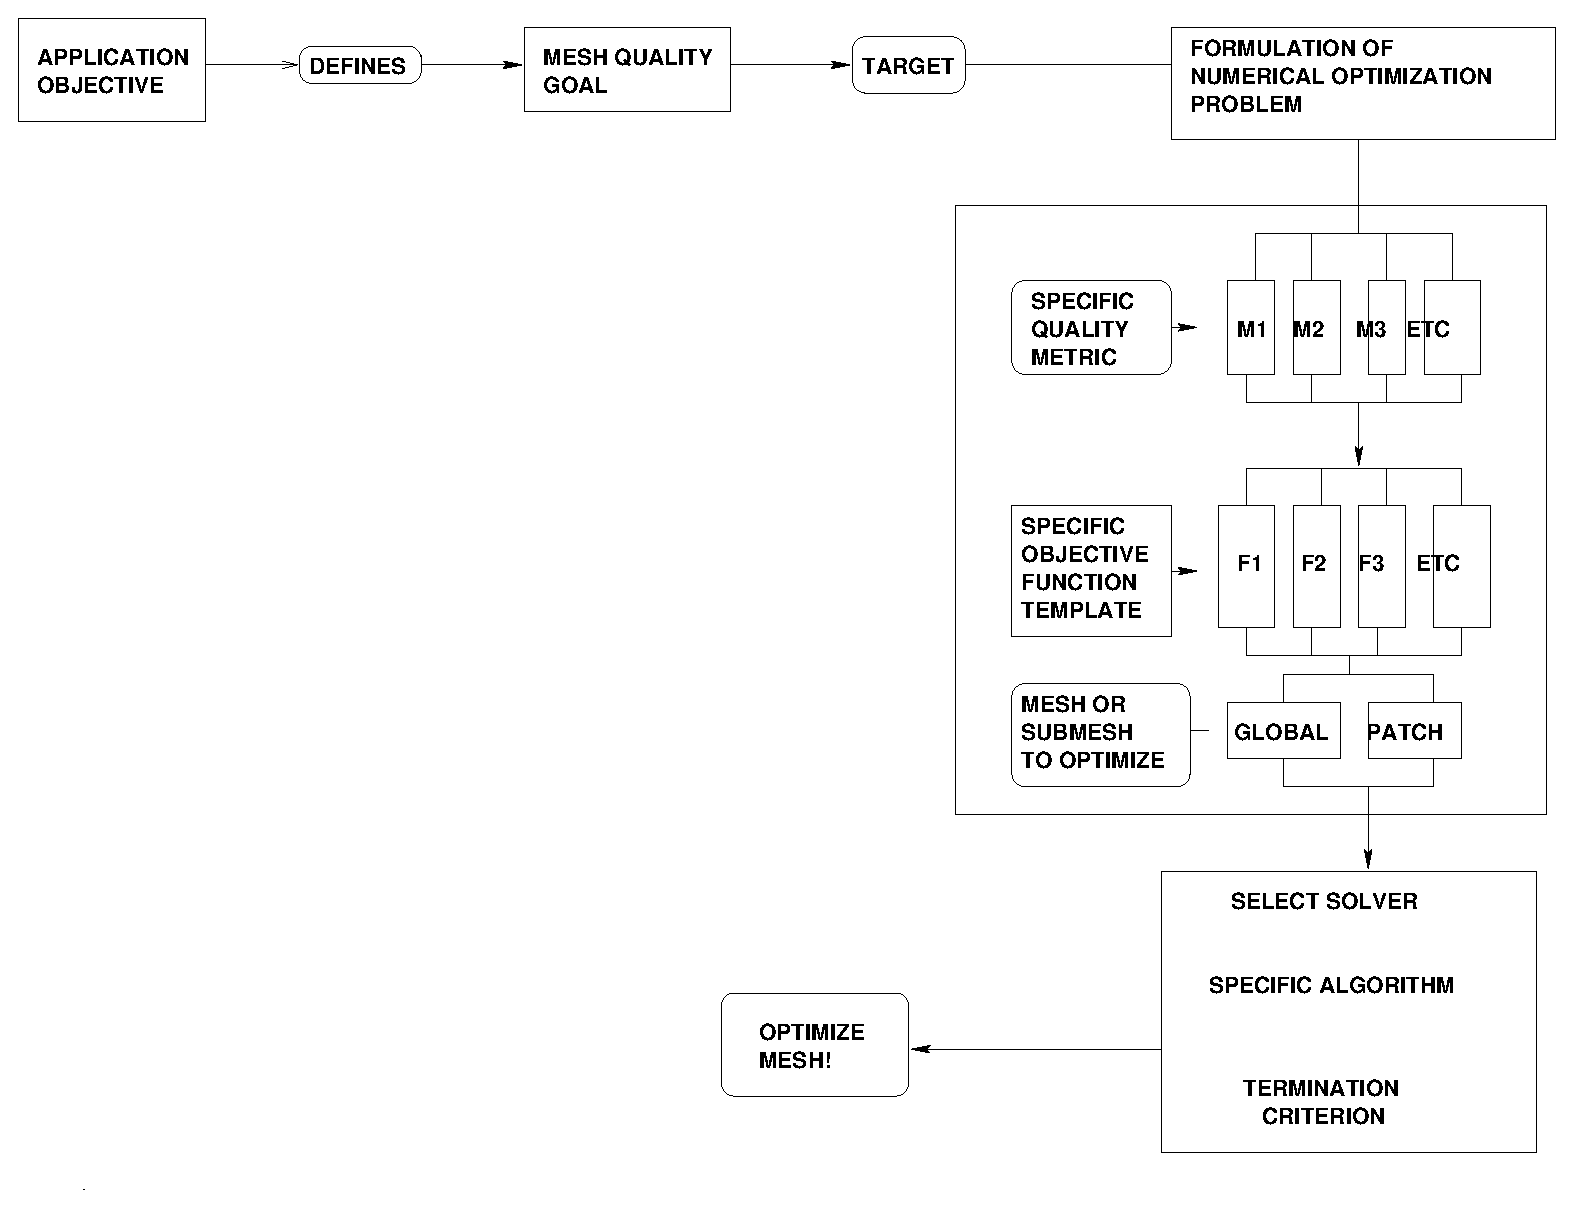
\includegraphics[width=4.7in]{msq-paradigm}
\caption{\em The Mesquite Paradigm \label{Paradigm} }
%\end{tabular}
\end{center}
\end{figure}

\section{How to use this User's Manual}
This user's manual 
\begin{itemize}
\item provides an introduction to mesh quality and basic Mesquite concepts (Chapter \ref{sec:intro}), 
\item instructs novice users on how to download and install Mesquite (Chapter \ref{sec:install}), 
\item provides a tutorial on Mesquite's simplified user's interface and Mesquite's detailed API (Chapter \ref{sec:examples}).
\item describes how to load a mesh in Mesquite via files (Chapter \ref{sec:meshes}), and 
%\item provides instructions on using the extensive TSTT interface or a Mesquite mesh specific mesh
%      interface to load a mesh {\it dynamicallu} in Mesquite (sections \ref{sec:msq_mesh}, \ref{sec:TSTT}), and 
\item describes Mesquite interactions with domain geometry (Chapter \ref{sec:geom}), and
\item describes Mesquite Wrappers (Chapter \ref{sec:wrappers}),
%\item Exposes in details the concepts and the mechanisms of the advanced API (chapter \ref{sec:API}), and 
%\item instructs the user on how to add their own instances of quality 
%metrics, objective functions, and solvers (chapter \ref{sec:extensions})
\end{itemize}

Consult the doxygen documentation for the API reference as well as details on the software. There
are two sets of doxygen documentations available:
\begin{itemize}
\item The developer doxygen doc is located in mesquite/doc/developer/. From that directory, you
      must run 'doxygen Mesquite.dox'.
\item The user doxygen doc (API doc) is located in mesquite/doc/user/doxygen. From that directory, you
      must run 'doxygen Mesquite-user.dox'.
\end{itemize}
The doxygen command will generate two directories: an html directory containing the file
index.html that you can open with your web browser, and a latex directory containing a Makefile that
will generate a dvi file. 

%\section{Related Documents}

%Documentation of the Mesquite API can be generated from comments in the Mesquite
%source code using the Doxygen utility 
%(\url{http://www.stack.nl/~dimitri/doxygen/}).
%To generate HTML and LaTeX copies of this documentation, execute the command 
%{\tt doxygen Mesquite-user.dox} in the {\tt doc/usr/doxygen} subdirectory
%of the Mesquite source.

%Further information and related documentation are available on the 
%Mesquite home page, located at:
%\url{http://www.cs.sandia.gov/optimization/knupp/Mesquite.html}.


% Installing Mesquite
\chapter{Installing Mesquite} \label{sec:install}

\section{Requirements}

\subsection{Downloading Mesquite}
The Mesquite distribution (in source form) may be obtained at the following URL:
\begin{center}
\url{http://www.cs.sandia.gov/~web1400/1400_download.html}
\end{center}

\subsection{Supported Platforms and Build Requirements}
The Mesquite source code will compile in any environment comforming to the ISO/IEC 9899-1999 (C99), ISO/IEC 14882-1998 (C++98) and ISO/IEC 9945:2003 (POSIX) standards. It may also compile under many other environments.

Mesquite requires a reasonably standards-conforming C++ compiler and corresponding libraries.  No additional libraries are required to build the core Mesquite library. Several optional features have additional requirements.  These are listed in the next section.

Mesquite uses the GNU autotools build system.  The Makefiles generated by the
configure script should work on any Unix-like platform using the build tools
(e.g. make) provided with that platform.  The minimal requires beyond a C++
compiler are a Bourne shell (typically \texttt{/bin/sh}) implementation and
a minimal corresponding command environment and an implementation of the \texttt{make} utility.

Support for building Mesquite with Microsoft Visual Studio is no longer
available as of Mesquite version 2.0.  

%Mesquite is regularly compiled and tested on GNU/Linux with g++ 3.2 or later %and Sun with the Sun Forte C++ compiler.  

\subsection{Optional Libraries and Utilities}
\label{sec:depends}
\begin{itemize}
\item Unit tests:  Mesquite provides a series of unit tests that may be used
to verify the correct behavior of a build of the Mesquite library.  These tests
are implemented using CppUnit framework.  The CppUnit framework must be installed
to compile and run these test.  It is available at this URL:
\begin{center}
\url{http://cppunit.sourceforge.net}
\end{center}
\item ExodusII support:  To enable support for reading or writing ExodusII files in Mesquite, the header files for the ExodusII library must be available.  To link an application with a Mesquite library supporting ExodusII, the ExodusII library and possibly the NetCDF library must be available.  To obtain the ExodusII library, contact:
\begin{verbatim}
Marilyn K. Smith
Research Programs Department
Department 9103, MS 0833
Sandia National Laboratories
P.O.Box 5800
Albuquerque, NM 87185-0833
Phone: (505) 844-3082
FAX:   (505) 844-8251
Email: mksmith@sandia.gov
\end{verbatim}
The NetCDF library can be obained at the following URL:
\begin{center}
\begin{small}\url{http://www.unidata.ucar.edu/downloads/netcdf/index.jsp}\end{small}
\end{center}
\end{itemize}


\section{Building Mesquite}
\label{sec:compiling}
After downloading and unpacking the Mesquite source, the next step is to 
configure and build and install the Mesquite library.  
\subsection{Compiling on Unix-like systems}
This section presents the steps required to compile Mesquite with the default
options.  It is typically required
that Mesquite be "installed" before it is used in an application.  The default 
installation location is the system-wide \texttt{/usr/local} directory.  
It is more common to specify an alternate directory in which to install 
the Mesquite library and headers.  This can be done using the \texttt{--prefix}
option to the \texttt{configure} script.  Additional options are available for
fine-grained control of installation locations.
\begin{enumerate}
\item Change your working directory to the top-level Mesquite source
      directory (typically \texttt{mesquite-<version>/}).
\item Run the configure script with the command: 
\begin{center}
\texttt{./configure --prefix=<installdir>},
\end{center}
      replacing \texttt{<installedir>} with the location in which the finished
      Mesquite library is to be placed.
\item Compile Mesquite with the command: \texttt{make} 
\item Optionally verify that Mesquite compiled correctly with the command: \texttt{make check}
\item Move resulting files into the destination (install) directory with the command: \texttt{make install}
\end{enumerate}
If the configure step failed, please consult the following section describing 
some of the optional arguments to the \texttt{./configure} script. 
\subsection{Options for Unix-like systems}
This section describes the options available for customizing the build
system and the resulting Mesquite library.  An brief description of these
and other options is available with the command: \texttt{./configure --help}.

\label{mes_vars_and_defs}
The following values may be specified as environmental variables, as arguments
to the configure script using the NAME=VALUE syntax, or as arguments to \texttt{make}
using the NAME=VALUE syntax.  The value of these variables (if set) during the
configure step will become the default for the compile step.  The value of any
of these variables will override the the default if specified during the compile
step.
\begin{description}
\item[CXX]       The C++ compiler command
\item[CXXFLAGS]  Arguments to the C++ compiler, such as those specifying 
debug symbols or the optimization level.
\item[CC]        The C compiler command
\item[CFLAGS]    Command line arguments to be used for the C compiler.
\item[DOXYGEN]   The doxygen API documentation generation tool.
\end{description}

Most options to the configure script are either of the form 
\begin{center}
\texttt{--with-FEATURE[=ARG]} or \texttt{--enable-FEATURE[=ARG]}.
\end{center}
Some options may accept an additional argument following 
an `=' character.  For each --with-FEATURE option, there is also a corresponding
--without-FEATURE option.  Similarly, there is a --disable-FEATURE option 
corresponding to each --enable-FEATURE option.  The negative forms fo the options 
(--without-FEATURE and --disable-FEATURE) do not accept an additional argument.  
Only the positive form of each option is stated in the description below.  

\label{config_options}
The following general build and debug options may be specified during the configure step:
\begin{description}
\item[--enable-debug]  Select a subset of the following options that
make the most sense for developers of Mesquite.
\item[--enable-release]  This is the default behavior unless 
--enable-debug is specified.  It selects a subset of the following options that
typically work best for using Mesquite in a production application.
\item[--enable-compile-optimized] Compile with the available 
optimizations that improve performance without any significant drawbacks 
(the -O2 compiler flag.)
\item[--enable-debug-symbols] Include debugging information in
the compiled \\ Mesquite objects (the -g compiler flag).
\item[--enable-debug-assertions]  Include internal consistancy 
checks that abort when an error is detected.
\item[--enable-debug-output=n,m,...]  Enable the output of
debug and status messages to file descriptor 1 (stdout).  An 
list of integer debug flags for which to enable output may be specified 
as a comma-separated list of values.  The default is to enable debug
flags 1 and 2 if this option is specified without any explict debug
flag values.
\item[--enable-function-timers]  Enable time-profiling of
some portions of Mesquite.
\item[--enable-trap-fpe]  Enable generation of a floating-point
exception signal for arithmatic errors (e.g. division by zero.)  This is
an option intended for Mesquite developers.  Enabling this will typically cause
the application using Mesquite to abort when such an error is encountered.
\item[--enable-namespace]  Specify an alternate namespace so as to avoid
symbol conflicts between multiple versions of Mesquite.  See Section \ref{namespace_mangling}.
\end{description}

The following options specify optional Mesquite components and the location 
of the corresponding dependencies.
\begin{description}
\item[--with-cppunit=DIR]  The CppUnit library is required to compile
and run the tests to verify that a particular build of the Mesquite library
is working correctly.  If the CppUnit library is not installed in a default location
where the ./configure script can find it, this option may be used to specify
the location.
\item[--with-exodus=DIR]  Enable support for reading and writing
ExodusII files, and optionally specify the location where the ExodusII library
and headers required for this option are installed.
\item[--with-netcdf=DIR]  Specify the location of the NetCDF library
required by the ExodusII library.  The default is to look in the ExodusII
directory.
\end{description}

\subsection{Compiling on Microsoft Windows (CMake build)}

The Mesquite source includes the necessary input files to generate Microsoft
Visual Studio project files using the CMake utility.  You will need to 
download and install the CMake utility for Windows if you have not already done so.  It is available at:
\begin{center}
 \url{http://www.cmake.org/cmake/resources/software.html}
\end{center}

Using the graphical verison of the CMake utility, select the folder containing the Mesquite source and enter a folder in which you would like the CMake output and compiled code to be stored.  Select the \texttt{Configure} button.  You will be presented with a group of configuration options.  Modify any desired options and click the \texttt{Configure} button again.  Each time you change one or more configuration options, you must click the \texttt{Configure} button to update the list of available options.  When you have finished changing build options, click the \texttt{Generate} button to generate Visual Studio input files and exit the CMake utility.

The build folder you specified in the CMake utility should now contain the necessary input files to build Mesquite using Microsoft Visual C++.  

\subsection{Linking Multiple Versions of Mesquite \label{namespace_mangling} }

Sometimes it is necessary to have multiple different versions of a library 
such as Mesquite linked into the same application.  This situation typically
arises when an application needs both Mesquite and some other library that depends on an older version of Mesquite.  Without taking steps to avoid symbol
name conflicts such a situation will often result in surprising, strange, and
difficult to diagnose runtime errors.  

Mesquite provides the ability to specify an alternate namespace and a standard
namespace alias to assist with addressing such situations.  The ``namespace'' \texttt{Mesquite} is typcially an alias to the true internal C++ namespace containing all Mesquite code.  Applications can and should use that alias rather than the internal namespace to avoid the need to modify application code whenever the internal namespace changes.  

The internal namespace can be changed with the configure option \texttt{--enable-namespace=MyNS} or the cmake option \texttt{Mesqutie\_NAMESPACE}, where the value ``MyNS'' can be replaced with any string that is an acceptable C++ namespace label.  The default namespace is \texttt{MesquiteN}, with the Mesquite major version subtitited for \texttt{N}.  Specifying an alternate internal namespace results in different mangled symbol names in the compiled library, thus avoiding symbol name conflicts.

If the requested namespace is anything other than ``Mesquite'', then Mesquite will always provide the alias \texttt{namespace Mesquite = MESQUITE\_NS;} so that application code may always use the \texttt{Mesquite} namespace.




% Examples
\chapter{Examples} \label{sec:examples}

\section{Short Tutorial}

In this section, we write a driver code which calls the Mesquite
library to improve the quality of a test mesh. This tutorial section
is aimed at giving the user a feel for Mesquite: \emph{this section is not
where to look for detailed information}. In particular, information
pertaining to loading a particular mesh format (see Chapter \ref{sec:meshes}), 
interacting through a particular mesh interface (section \ref{sec:MeshData}), 
and details of defining geometric domains (see Chapter \ref{sec:geom}) are not
given in this section.

First, we write a small program using Mesquite's simplified API, or
wrappers, to show the fastest way deploy Mesquite functionality to
improve a mesh.  The wrapper concept, as well as details about the
different wrappers available, are described in section
\ref{sec:tutWrapper}.  Following this first example, we set up customized mesh
improvement tool using Mesquite's low-level API, the details of which
are described in section \ref{sec:tutDetailedAPI}.

\subsection{Tutorial File Template}
\label{sec:tutfile}

To create and link a driver code, the Mesquite library must be
installed per the instructions of section \ref{sec:compiling}. 
This commands and file names specified in this section are relative 
to the installed \texttt{testsuite/tutorial} directory.  It 
is assumed that that is the working diretory.
This tutorial begins with the file \texttt{tutorial.cpp}, 
which contains the following template:
\begin{verbatim}
1.  #include "Mesquite_all_headers.hpp"
    #include <ostream>
2.  using namespace Mesquite;
    int main(int argc, char* argv[])
    {
3.    MsqError err;

      if (argc != 2) {
        std::cerr << "Expected mesh file names as single argument."
                  << std::endl;
        exit (EXIT_FAILURE);
      }

      // new code starts here
4.    //... 

      return 0;
    }
\end{verbatim}
The lines labeled 1-3 highlight three basic aspects of using Mesquite;
\begin{enumerate}
\item For convenience, Mesquite provides the header file
\begin{center}
\texttt{include/Mesquite\_all\_headers.hpp}
\end{center} which includes all Mesquite
headers. Although this is the easiest way to handle the include directives,
it may slow down compilation of the application.  
\item All Mesquite classes are part of the \texttt{Mesquite} namespace. 

\item  The \texttt{MsqError} class defines an object type used to communicate
Mesquite errors to the application.  The calling application must pass
an instance of the \texttt{MsqError} class or an instance of a subclass of
\texttt{MsqError} to many Mesquite functions.  The state of the error object
may be checked by casting the instance ot a Boolean or using it in a 
Boolean context.  The state is cleared by calling the \texttt{clear} method.
\item In the sections that follow, we guide the user through the steps
necessary to smooth a mesh using Mesquite.  All new lines of code to be
added to the template file start in this position and are added in the order
in which they are discussed.
\end{enumerate}

The code above takes a mesh file name as a command line argument and
performs no action. We can compile it in the 
(\texttt{examples/}) directory with the command:

\begin{verbatim}
                        make -f tutorial.make
\end{verbatim}


\subsection{Loading a Test Mesh}
\label{sec:tutMesh}
Our next step is to load one of the test meshes distributed with
Mesquite.  These meshes are distributed in the VTK unstructured mesh
format, the details of which are given in \cite{VTKbook, VTKuml}. This
format was chosen because of its readability and ease of use.
In this tutorial we use
the simplest mechanism for loadling a mesh into Mesquite; different
options are described in Chapter \ref{sec:meshes}.  In particular, to
load a VTK test mesh in Mesquite, instantiate the Mesquite mesh
database object,
\texttt{MeshImpl}, and use the \texttt{read\_vtk} member function by
adding the following lines to the file template described in
\ref{sec:tutfile}.
\begin{verbatim}
  Mesquite::MeshImpl my_mesh;
  my_mesh.read_vtk(argv[1], err); 
  if (err) 
  {
    std::cout << err << std::endl;
    return 1;
  }
\end{verbatim}

Mesquite also provides a function to write a mesh
file in VTK format, given a \texttt{MeshImpl} object:
\begin{verbatim}
  my_mesh.write_vtk("original_mesh.vtk",err); 
\end{verbatim}

Mesquite deals automatically with all types of supported elements 
(triangles, quadrilaterals, tetrahedra, hexahedra, wedges, and pyramids),
and also hybrid meshes consisting of mixed element types.  
Some meshes require geometry information as well.  When improving a surface mesh, Mesquite must be provided information
about surface(s) the mesh is constrained to lie on and the association between
mesh entities and entities of the geometric domain (surfaces, curves, etc.)
Because Mesquite is inherently a 3D code, all 2D meshes must specify some
geometry constraints.  The details
for general geometric surfaces are explained in Chapter 
\ref{sec:geom}. In this section,
we show how to define the geometry of a 2D planar mesh, specified by a
point $(x,y,z)$ and a normal. For example, the following defines an xy-plane
shifted five units in the z-direction:
\begin{verbatim}
  Vector3D normal(0,0,1);
  Vector3D point(0,0,5);
  PlanarDomain my_mesh_plane(normal, point);
\end{verbatim}


\subsection{Improving the Mesh with a Wrapper Class}
\label{sec:tutWrapper}
The simplest way to use a Mesquite mesh quality improvement
procedure is to instantiate one of the wrapper classes described in Chapter 
\ref{sec:wrappers}. Here, we will instantiate the
\texttt{ShapeImprovement} wrapper and use it to improve 
the Mesh we created earlier.  Mesquite can optimize the mesh
without further input from the user by utilizing preset, default
values.  If some customization is desired, the wrapper classes also
allow users to set the most important parameters of the underlying
algorithms and metrics (see Chapter 
\ref{sec:wrappers} for details).
\begin{verbatim}
Mesquite::ShapeImprover mesh_quality_algorithm;
mesh_quality_algorithm.run_instructions(&my_mesh,
                                        &my_mesh_plane,  err);
//Should check the error object after the instruction is ran
// to see whether the instructions were all successful.
if (err) 
{
    std::cout << err << std::endl;
    return 1;
}
\end{verbatim}

Once the algorithm has been executed using the {\tt run\_instructions} member
function of the wrapper class, the improved mesh can be written to a new
file:
\begin{verbatim}
  my_mesh.write_vtk("smoothed_mesh.vtk",err); 
\end{verbatim}
This completes the code necessary for the simple wrapper example.  Once
the code has successfully compiled by typing the {\tt make} command given in
section \ref{sec:tutfile}, 
run it from the tutorial directory \texttt{mesquite/testSuite/tutorial/}
with a mesh file name as a command line 
argument by typing 
\begin{verbatim}
./tutorial ../../meshFiles/2D/VTK/square_quad_10_rand.vtk
\end{verbatim}
The code creates the files original\_mesh.vtk
and improved\_mesh.vtk in the current directory.  These two meshes, the
original and the optimized, are
shown in figure \ref{fig:square_rand}.  The text output of the code,
shown below, reports the inverse mean ratio quality metric statistics for
the mesh at three stages:  the original mesh, the mesh at an intermediate
step of the optimization, and the final mesh.  The optimized mesh consists
of square quadrilaterals which have an inverse mean ratio value of 1.0.
\begin{verbatim}
************** QualityAssessor Summary **************

  There were no inverted elements detected. 
  No entities had undefined values for any computed metric.

             metric    minimum    average        rms    maximum
 Inverse Mean Ratio    1.01013    1.16655     1.1738    1.79134

************** QualityAssessor Summary **************

  There were no inverted elements detected. 
  No entities had undefined values for any computed metric.

             metric    minimum    average        rms    maximum
 Inverse Mean Ratio    1.01013    1.16655     1.1738    1.79134

************** QualityAssessor Summary **************

  There were no inverted elements detected. 
  No entities had undefined values for any computed metric.

             metric    minimum    average        rms    maximum
 Inverse Mean Ratio          1          1          1          1
\end{verbatim}
\begin{figure*}[htbp]
\begin{center}
    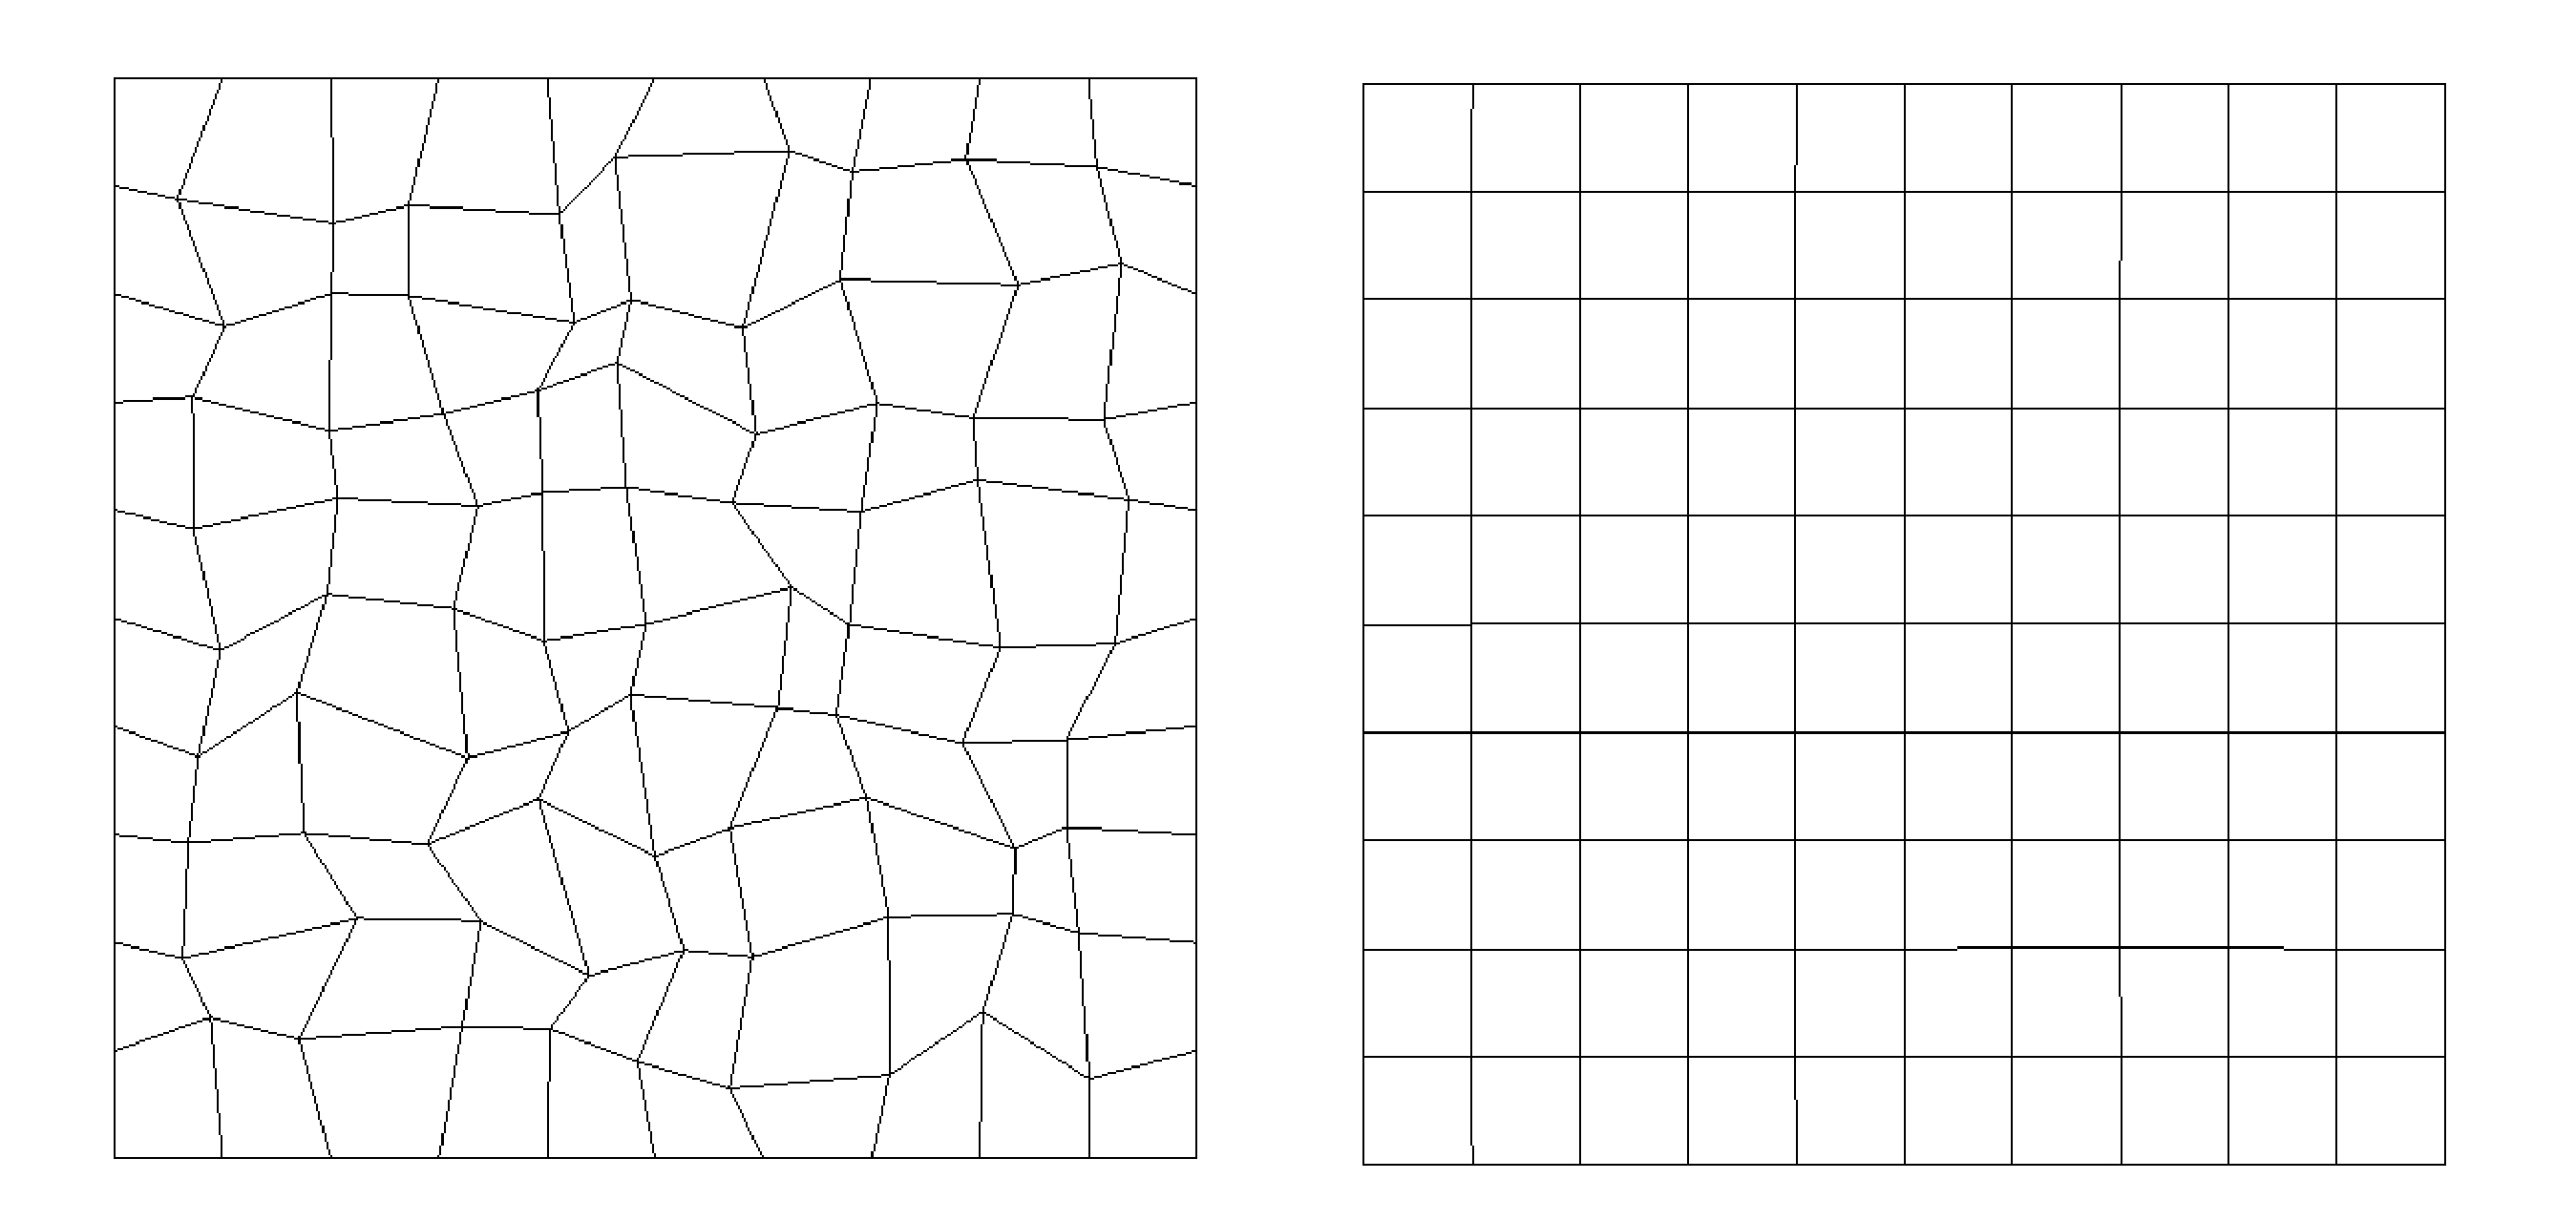
\includegraphics[height=50mm]{square_rand.eps}
    \caption{square\_quad\_10\_rand.vtk mesh. The original mesh is on the left, the mesh smoothed with \texttt{ShapeImprover} is shown on the right.}
    \label{fig:square_rand}
\end{center}
\end{figure*}


\subsection{Improving the Mesh with the Low Level API}
\label{sec:tutDetailedAPI}
If the user requires in-depth control over the mesh quality improvement
process, the use of lower-level Mesquite classes provides an extensive
amount of flexibility.   In particular, the user can specify the quality
metric, objective function template, and optimization algorithm by
instantiating particular instances of each.  For each, various options
such as numerical or analytical gradient and Hessian evaluations or
the patch size can be selected.  Furthermore, the user can fine tune
the optimization algorithm performance by creating and setting the parameters 
of the termination criteria.
%for both inner and outer iterations.
%mbrewer removed reference to inner and outer iterations.
%{\tt LAF have we talked about inner and outer iterations before? perhaps
%too advanced for the tutorial}

Once these core objects have been created and customized, the user
creates an instruction queue and adds one or more quality improvers
and quality assessors to it.  The mesh optimization process is initiated
with the {\tt run\_instructions} method on the instruction queue
class.

In this section, we provide a simple example to highlight the main
steps needed for this approach.  The code segment given below performs
the same functionality as the wrapper class highlighted in the
previous section.  The comment lines provide high level documentation;
the details of each class and the low-level API are not described here.
%extensively treated in Section 
%\ref{sec:detailedAPI}.

\begin{verbatim}
    // creates a mean ratio quality metric ...
  IdealWeightInverseMeanRatio inverse_mean_ratio(err);

    // sets the objective function template
  LPtoPTemplate obj_func(&inverse_mean_ratio, 2, err);
  
    // creates the optimization procedures
  FeasibleNewton f_newton(&obj_func);

    //performs optimization globally
  f_newton.use_global_patch(); 

    // creates a termination criterion and 
    // add it to the optimization procedure
    // outer loop: default behavior: 1 iteration
    // inner loop: stop if gradient norm < eps
  TerminationCriterion tc_inner;
  tc_inner.add_absolute_gradient_L2_norm( 1e-4 ); 
  f_newton.set_inner_termination_criterion(&tc_inner);

    // creates a quality assessor
  QualityAssessor m_ratio_qa(&inverse_mean_ratio);
    // creates an instruction queue
  InstructionQueue queue;
  queue.add_quality_assessor(&m_ratio_qa, err); 
  queue.set_master_quality_improver(&f_newton, err); 
  queue.add_quality_assessor(&m_ratio_qa, err); 

    // do optimization of the mesh_set
  queue.run_instructions(&my_mesh, &my_mesh_plane, err); 
  if (err) {
    std::cout << err << std::endl;
    return 2;
  }
\end{verbatim} 

\subsection{Mesh Improvement Examples}

The left image in figure \ref{fig:hole} shows a mesh that has
been degraded by moving the disk from the right side of the square to
the left while keeping the mesh topology fixed.
The mesh file
\texttt{mesquite/meshFiles/2D/VTK/hole\_in\_square.vtk} contains the
information for this mesh.  If you plan to run this example, note that
the normal direction that defines the geometry is now $(0,0,-1)$.
This change must be made in the tutorial example code
as was done in section \ref{sec:tutMesh}, or an error message will be
thrown.
\begin{verbatim}
  Vector3D normal(0,0,-1);
  Vector3D point(0,0,-5);
  PlanarDomain my_mesh_plane(normal, point);
\end{verbatim}

We can now improve the mesh with the wrapper mentioned in
\ref{sec:tutWrapper} or the detailed API mentioned in
\ref{sec:tutDetailedAPI}. 
Because we changed the normal, the driver code must be recompiled;
otherwise the code and executable are as before.
Once the code is recompiled, type 
\begin{verbatim}
./tutorial ../../meshFiles/2D/VTK/hole_in_square.vtk
\end{verbatim}
to improve this mesh.
The smoothed mesh is shown in the right image of figure
\ref{fig:hole}.
The vertex locations have been repositioned and significantly improve
the quality of the mesh, as shown by the onscreen
quality assessor output:  
\begin{verbatim}
************** QualityAssessor Summary **************

  There were no inverted elements detected. 
  No entities had undefined values for any computed metric.

             metric     average
 Inverse Mean Ratio     85.8391

************** QualityAssessor Summary **************

  There were no inverted elements detected. 
  No entities had undefined values for any computed  metric.

             metric     average
 Inverse Mean Ratio     1.83479

\end{verbatim}
\begin{figure*}[htbp]
\begin{center}
    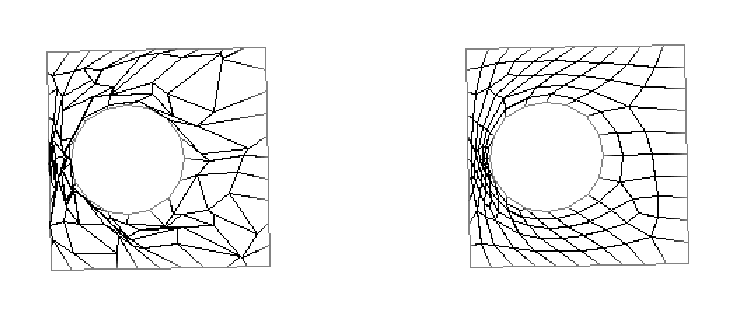
\includegraphics{hole_in_square.ps}
    \caption{hole\_in\_square.vtk mesh. The original mesh is on the left, the mesh smoothed with
    Mesquite is shown on the right.}
    \label{fig:hole}
\end{center}
\end{figure*}


% Getting Mesh Into Mesqite
\chapter{Getting Mesh Into Mesquite}
\label{sec:meshes}

The application must provide Mesquite with data on which to operate.  The two
fundamental classes of information Mesquite requires are:
\begin{itemize}
\item Mesh vertex coordinates and element connectivity, and
\item Constraints on vertex movement.
\end{itemize}
In this chapter we will assume that the only constraint available for vertex movement is to flag the vertices as fixed.  More advanced constraints such as vertices following geometric curves or surfaces are discussed in the following chapter.  

The mesh data expected as input to Mesquite is a set of vertices and elements.  Each vertex has associated with it a fixed flag, a ``byte'', and x, y, and z coordinate values.  The fixed flag is used as input only.  It indicates whether or not the corresponding vertex position should be fixed (i.e., coordinates not allowed to change) during the optimization.  The ``byte'' is one byte of Mesquite-specific working data assocaited with each vertex (currently only used for vertex culling.)   The coordinate values for each vertex serve as both input and output: as input they are the initial positions of the vertices and as output they are the optimized positions.  

Each element of the input mesh has associated with it a type and a list of vertices.  The type is one of the values defined in \texttt{Mesquite::EntityTopology} (\texttt{Mesquite.hpp}).  It specifes the topology (type of shape) of the element. Currently supported element types are triangles, quadrilaterals, 
tetrahdra, hexahedra, triangular wedges, and pyramids.  The list of vertices (commonly referred to as the ``connectivity'') define the geometry (location and variation of shape) for the element.  The vertices are expected to be occur in a pre-defined order specific to the element topology. Mesquite uses the canonical ordering defined in the ExodusII specification\cite{exodus}.

For some more advanced capabilities, Mesquite may require the ability to attach arbitrary peices of data (called ``tags'') to mesh elements or vertices.

\section{The \texttt{Mesquite::Mesh} Interface} \label{sec:MeshData}

The \texttt{Mesquite::Mesh} class (\texttt{MeshInterface.hpp}) defines the interface Mesquite uses to interact with mesh data.  In C++ this means that the class defines a variety of pure virtual (or abstract) functions for accessing mesh data.  An application may implement a subclass of \texttt{Mesquite::Mesh}, providing implementations of the virtual methods that allow Mesquite direct access to the applications in-memory mesh representation.  

The \texttt{Mesquite::Mesh} interface defines functions for operations such as:
\begin{itemize}
\item Get a list of all mesh vertices.
\item Get a list of all mesh elements.
\item Get a property of a vertex (coordinates, fixed flag, etc.)
\item Set a property of a vertex (coordinates, ``byte'', etc.)
\item Get the type of an element
\item Get the vertices in an element
\end{itemize}
It also defines other operations that are only used for certain optimization algorithms:
\begin{itemize}
\item Get the list of elements for which a specific vertex occurs in the connetivity list.
\item Define a ``tag'' and use it to associate data with vertices or elements.
\end{itemize}

Mesh entities (vertices and elements) are referenced in the \texttt{Mesquite::Mesh} interface using `handles'.  There must be a unique handle
space for all vertices, and a separate unique handle space for all elements. 
That is, there must be a one-to-one mapping between handle values and vertices,
and a one-to-one mapping between handle values and elements.  The storage type of
the handles is specified by 
\begin{center}
\texttt{Mesquite::Mesh::VertexHandle} and \texttt{Mesquite::Mesh::ElementHandle}.
\end{center}
The handle types are of sufficient size
to hold either a pointer or an index, allowing the underlying implementation of
the \texttt{Mesquite::Mesh} interface to be either pointer-based or index-based. 
All mesh entities are referenced using handles.  For example, the
\texttt{Mesquite::Mesh} interface declares a method to retrieve the list of all
vertices as an array of handles and a method to update the coordinates of a
vertex where the vertex is specified as a handle.

It is recommended that the application invoke the Mesquite optimizer for subsets
of the mesh rather than the entire mesh whenever it makes sense to do so.  For
example, if a mesh of two geometric volumes is to be optimized and all mesh
vertices lying on geometric surfaces are constrained to be fixed (such vertices
will not be moved during the optimization) then optimizing each volume separately
will produce the same result as optimizing both together.  


\section{ITAPS iMesh Interface}

The ITAPS Working Group has defined a standard API for exchange of mesh data between applications.  The iMesh interface\cite{imesh} defines a superset of the functionality required for the \texttt{Mesquite::Mesh} interface.  Mesquite can access mesh through an iMesh interface using the \texttt{Mesquite::MsqIMesh} class declared in \texttt{MsqIMesh.hpp}.  This class is an ``adaptor'':  it presents the iMesh interface as the \texttt{Mesquite::Mesh} interface.  


\section{Accessing Mesh In Arrays} \label{sec::ArrayMesh}

One common representation of mesh in applications is composed of simple 
coordinate and index arrays.  Mesquite provides the \texttt{ArrayMesh} implementation of the \texttt{Mesquite::Mesh} interface to allow Mesquite
to access such array-based mesh definitions directly.  The mesh must be
defined as follows:
\begin{itemize}
\item Vertex coordinates must be stored in an array of double-precision
      floating-point values.  The coordinate values must be interleaved,
      meaning that the x, y, and z coordinate values for a single vertex
      are contiguous in memory.
\item The mesh must be composed of a single element type.
\item The element connectivity (vertices in each element) must be stored
      in an interleaved format as an array of long integers.  The vertices
      in each element are specified by an integer \texttt{i}, where the location       of the coordinates of the corresponding vertex is located at position
      \texttt{3*i} in the vertex coordinates array.
\item The fixed/boundary state of the vertices must be stored in an array
      of integer values, where a value of 1 indicates a fixed vertex and a 
      value of 0 indicates a free vertex.  The values in this array must
      be in the same order as the corresponding vertex coordinates in the
      coordinate array.
\end{itemize}

The following is a simple example of using the ArrayMesh object to pass
Mesquite a mesh containing four quadrilateral elements.
\begin{verbatim}
/** define some mesh **/
    /* vertex coordinates */
  double coords[] = { 0, 0, 0,
                      1, 0, 0,
                      2, 0, 0,
                      0, 1, 0,
                     .5,.5, 0,
                      2, 1, 0,
                      0, 2, 0,
                      1, 2, 0,
                      2, 2, 0 };
    /* quadrileratal element connectivity (vertices) */
  long quads[] = { 0, 1, 4, 3,
                   1, 2, 5, 4,
                   3, 4, 7, 6,
                   4, 5, 8, 7 };
    /* all vertices except the center on are fixed */
  int fixed[] = { 1, 1, 1,
                  1, 0, 1,
                  1, 1, 1 };
  
/** create an ArrayMesh to pass the above mesh into Mesquite **/
  
  ArrayMesh mesh( 
      3,            /* 3D mesh (three coord values per vertex) */
      9,            /* nine vertices */
      coords,       /* the vertex coordinates */ 
      fixed,        /* the vertex fixed flags */
      4,            /* four elements */
      QUADRILATERAL,/* elements are quadrilaterals */
      quads );      /* element connectivity */
  
/** smooth the mesh **/
  
    /* Need surface to constrain 2D elements to */
    PlanarDomain domain( PlanarDomain::XY );

  MsqError err;
  ShapeImprover shape_wrapper;
  if (err) {
    std::cout << err << std::endl;
    exit (2);
  }
  
  shape_wrapper.run_instructions( &mesh, &domain, err );
  if (err) {
    std::cout << "Error smoothing mesh:" << std::endl
              << err << std::endl;
  }
  
/** Output the new location of the center vertex **/
  std::cout << "New vertex location: ( "
            << coords[12] << ", " 
            << coords[13] << ", " 
            << coords[14] << " )" << std::endl;
\end{verbatim}

NOTE:  When using the \texttt{ArrayMesh} interface, the application is responsible for managing the storage of the mesh data.  The \texttt{ArrayMesh}
 does NOT copy the input mesh.  

 
\section{Reading Mesh From Files} \label{sec:meshFiles}

Mesquite provides a concrete implementation of the \texttt{Mesquite::Mesh} named
\texttt{Mesquite::MeshImpl}.  This implementation is capable of reading mesh from
VTK\cite{VTKbook, VTKuml} and optionally ExodusII files. See Sections 
\ref{sec:depends} and \ref{sec:compiling} for more 
information regarding the optional support for ExodusII files.

The `fixed' flag for vertices can be specified in VTK files by defining a
SCALAR POINT\_DATA attribute with values of 0 or 1, where 1 indicates that the
corresponding vertex is fixed.  The \texttt{Mesquite::MeshImpl} class is capable
of reading and storing tag data 
%(see Section \ref{tags}) 
using VTK attributes and
field data.  The current implementation writes version 3.0 of the VTK file format
and is capable of reading any version of the file format up to 3.0.  



% Mesquite Features
\chapter{Mesquite Features}

  This chapter is summarizes various aspects of Mesquite that will be useful in understanding the topics that follow.

\section{Solvers}

Many of the quality improvers in Mesquite work by minimizing the value of an
objective function (see Section \ref{sec:ObjectiveFunction}), where the
objective function is a function of the mesh vertex coordinates. 
The term \emph{solver} is often used to refer to the portion of the code in
the concrete subclass of \texttt{VertexMover} that implements the inner loop
of the optimization for quality improvers that optimize an explicit 
objective-function based (the code that implements the function-minimization algorithm.)

The remainder of this section lists the solvers available in Mesquite along with a small code example for each showing how to invoke the solver.


\subsection{Relaxation Smoothers}

Note that the relaxation smoothers do NOT require an objective function.

\subsubsection{LaplacianSmoother} 

Implements the Laplacian smoothing for a patch with one free vertex.  It moves the free center vertex to the average of the neighboring vertices.

\textbf{Code Example:}

\begin{lstlisting}[frame=single]
int main(int argc, char* argv[])
{
  const char input_file[] = MESH_FILES_DIR "2D/vtk/quads/untangled/square_quad_2.vtk";

    /* Read a VTK Mesh file */
  MsqPrintError err(cout);
  Mesquite::MeshImpl mesh;
  mesh.read_vtk( input_file, err);
  if (err) return 1;
  
    // creates an intruction queue
  InstructionQueue queue1;
  
    // creates a mean ratio quality metric ...
  ConditionNumberQualityMetric shape_metric;
  EdgeLengthQualityMetric lapl_met;
  lapl_met.set_averaging_method(QualityMetric::RMS);
 
    // creates the laplacian smoother  procedures
  LaplacianSmoother lapl1;
  QualityAssessor stop_qa=QualityAssessor(&shape_metric);
  stop_qa.add_quality_assessment(&lapl_met);
  
    //**************Set stopping criterion****************
  TerminationCriterion sc2;
  sc2.add_iteration_limit( 10 );
  if (err) return 1;
  lapl1.set_outer_termination_criterion(&sc2);
  
  queue1.add_quality_assessor(&stop_qa,err); 
  if (err) return 1;
  queue1.set_master_quality_improver(&lapl1, err); 
  if (err) return 1;
  queue1.add_quality_assessor(&stop_qa,err); 
  if (err) return 1;
 
  PlanarDomain plane(Vector3D(0,0,1), Vector3D(0,0,5));
  
    // launches optimization on mesh
  MeshDomainAssoc mesh_and_domain = MeshDomainAssoc(&mesh, &plane);
  queue1.run_instructions(&mesh_and_domain, err); 
  if (err) return 1;

  return 0;
}
\end{lstlisting}

\subsubsection{SmartLaplacianSmoother}

Does same as the Laplacian smoother, but doesn't invert elements.  Invoked same way as the LaplacianSmoother.  If initial mesh in non-inverted, the SmartLaplacianSmoother performs Laplace smoothing while trying not to invert the mesh.

\subsubsection{Randomize}

The randomize smoother moves a free vertex to a random location within a local patch.  This smoother is provided as a convenience to
those who wish to generate a poor quality mesh from an initial mesh in order to test another mesh improvement algorithm.

\textbf{Code Example:}

\begin{lstlisting}[frame=single]
int main( )
{
  Mesquite::MeshImpl mesh;
  MsqPrintError err(cout);
  mesh.read_vtk(VTK_2D_DIR "quads/untangled/tangled_quad.vtk", err);
  if (err) return 1;
  
  // Set Domain Constraint
  Vector3D pnt(0,0,0);
  Vector3D s_norm(0,0,1);
  PlanarDomain msq_geom(s_norm, pnt);
                                                                              
    // creates an intruction queue
  InstructionQueue queue1;
  
  Randomize rand(.05);
  
  TerminationCriterion sc_rand;
  sc_rand.add_iteration_limit( 10 );
 
  rand.set_outer_termination_criterion(&sc_rand);
  
  queue1.set_master_quality_improver(&rand, err);
  if (err) return 1;

  MeshDomainAssoc mesh_and_domain = MeshDomainAssoc(&mesh, &msq_geom);
  queue1.run_instructions(&mesh_and_domain, err);
  if (err) return 1;
  
  return 0;
}
\end{lstlisting}


\subsection{OptSolvers}

\subsubsection{ConjugateGradient}

Optimizes the objective function using the Polack-Ribiere scheme.

\textbf{Code Example:}

\begin{lstlisting}[frame=single]
int main( )
{
  Mesquite::MeshImpl mesh;
  MsqPrintError err(cout);
  mesh.read_vtk(VTK_2D_DIR "quads/untangled/tangled_quad.vtk", err);
  if (err) return 1;
  
    // Set Domain Constraint
  Vector3D pnt(0,0,0);
  Vector3D s_norm(0,0,1);
  PlanarDomain msq_geom(s_norm, pnt);
                                                                              
    // creates an intruction queue
  InstructionQueue queue1;
  
    // creates a mean ratio quality metric ...
  ConditionNumberQualityMetric shape_metric;
  UntangleBetaQualityMetric untangle(2);

  LInfTemplate obj_func(&untangle);

  if (err) return 1;
    // creates the steepest descent optimization procedures
  ConjugateGradient cg( &obj_func, err );
  if (err) return 1;
  
  QualityAssessor stop_qa=QualityAssessor(&shape_metric);
  QualityAssessor stop_qa2=QualityAssessor(&shape_metric);
   
  stop_qa.add_quality_assessment(&untangle);

  queue1.add_quality_assessor(&stop_qa,err); 
  if (err) return 1;
 
  queue1.set_master_quality_improver(&cg, err);
  if (err) return 1;
  queue1.add_quality_assessor(&stop_qa2,err);
  if (err) return 1;

  MeshDomainAssoc mesh_and_domain = MeshDomainAssoc(&mesh, &msq_geom);
  queue1.run_instructions(&mesh_and_domain, err);
  if (err) return 1;
  
  return 0;
}
\end{lstlisting}


\subsubsection{FeasibleNewton}
Implements the newton non-linear programming algorithm in order to move a free vertex to an optimal position given an ObjectiveFunction object and a QualityMetric object.  This implementation of Feasible Newton works well on volume meshes and on surfaces meshes using PlanarDomain that lie in the X-Y coordinate plane. It should not be used on non-planar surface meshes.

\textbf{Code Example:}

\begin{lstlisting}[frame=single]
int main()
{     
  MsqPrintError err(cout);
  Mesquite::MeshImpl mesh;
  mesh.read_vtk(MESH_FILES_DIR "3D/vtk/tets/untangled/3D/tire.vtk", err);
  if (err) return 1;
  
    // creates an intruction queue
  InstructionQueue queue1;

    // creates a mean ratio quality metric ...
  IdealWeightInverseMeanRatio mean(err);
  if (err) return 1;
  
  LPtoPTemplate obj_func(&mean, 1, err);
  if (err) return 1;
  
    // creates the optimization procedures
  FeasibleNewton fn( &obj_func );

    //perform optimization globally
  fn.use_global_patch();
  if (err) return 1;
  
  queue1.set_master_quality_improver(&fn, err); 
  if (err) return 1;

  queue1.run_instructions(&mesh, err); 
  if (err) return 1;
  
  return 0;
}
\end{lstlisting}


\subsubsection{SteepestDescent}
A very basic implementation of the steepest descent optimization algorithm.  It works on patches of any size but the step size is automatically computed and is not accessible through the interface. It is for testing purposes only. 

\textbf{Code Example:}

\begin{lstlisting}[frame=single]
int main()
{
  MsqPrintError err(std::cout);
  Mesquite::MeshImpl mesh;
  mesh.read_vtk(MESH_FILES_DIR "3D/vtk/hexes/untangled/hexes_4by2by2.vtk", err);
  
    // creates an instruction queue
  InstructionQueue queue1;
  
    // creates a mean ratio quality metric ...
  IdealWeightInverseMeanRatio mean_ratio(err);
  if (err) return 1;
  ConditionNumberQualityMetric cond_num;
  mean_ratio.set_averaging_method(QualityMetric::LINEAR);
  
    // ... and builds an objective function with it
  LPtoPTemplate obj_func(&mean_ratio, 2, err);
  if (err) return 1;

   // creates the steepest descent optimization procedures
  SteepestDescent sd( &obj_func );
  sd.use_global_patch();
  
  QualityAssessor stop_qa=QualityAssessor(&mean_ratio);
  if (err) return 1;
  stop_qa.add_quality_assessment(&cond_num);
  if (err) return 1;
    
   //**************Set stopping criterion****************
  TerminationCriterion tc2;
  tc2.add_iteration_limit( 1 );
  sd.set_inner_termination_criterion(&tc2);

  queue1.add_quality_assessor(&stop_qa,err);
  queue1.set_master_quality_improver(&sd, err); 
  if (err) return 1;
  queue1.add_quality_assessor(&stop_qa,err);
  if (err) return 1;

  mesh.write_vtk("original_mesh.vtk", err); 
  if (err) return 1;
  
  queue1.run_instructions(&mesh, err);
  if (err) return 1;
  

  return 0;
}
\end{lstlisting}


\subsubsection{QuasiNewton}
Port of Todd Munson's quasi-Newton solver to Mesquite.

\textbf{Code Example:}

\begin{lstlisting}[frame=single]
int main()
{
  MsqPrintError err(std::cout);
  Mesquite::MeshImpl mesh;
  mesh.read_vtk(MESH_FILES_DIR "3D/vtk/hexes/untangled/hexes_4by2by2.vtk", err);
  
    // creates an intruction queue
  InstructionQueue queue1;
  
    // creates a mean ratio quality metric ...
  IdealWeightInverseMeanRatio mean_ratio(err);
  if (err) return 1;
  EdgeLengthQualityMetric cond_num;
  mean_ratio.set_averaging_method(QualityMetric::LINEAR);
  
    // build an objective function
  LPtoPTemplate obj_func(&mean_ratio, 2, err);
  if (err) return 1;

  QuasiNewton qn( &obj_func );
  qn.use_global_patch();
  
  QualityAssessor stop_qa=QualityAssessor(&mean_ratio);
  if (err) return 1;
  stop_qa.add_quality_assessment(&cond_num);
  if (err) return 1;
    
   //**************Set stopping criterion****************
  TerminationCriterion tc2;
  tc2.add_iteration_limit( 1 );
  qn.set_inner_termination_criterion(&tc2);

  queue1.add_quality_assessor(&stop_qa,err);
  queue1.set_master_quality_improver(&qn, err); 
  if (err) return 1;
  queue1.add_quality_assessor(&stop_qa,err);
  if (err) return 1;

  queue1.run_instructions(&mesh, err);
  if (err) return 1;
  
  return 0;
}
\end{lstlisting}


\subsubsection{TrustRegion}
Port of Todd Munson's trust region solver to Mesquite.  The TrustRegion optimizer is invoked in the same way as in the previous QuasiNewton example.


\section{Objective Function}
\label{sec:ObjectiveFunction}

\subsection{Definition}

An objective function is a scalar function of all the vertex coordinates in the active mesh.  The mesh vertex locations are optimized so as to minimize the objective function value.  

The objective functions implemented in Mesquite can be divided into two general categories: template objective functions and composite objective functions.  Template objective functions have an associated \texttt{QualityMetric} instance and typically implement some kind of averaging scheme.  Composite objective functions modify the values of one or two other objective functions, such as scaling the value or summing two values.

Most solvers in Mesquite also require the gradient of the objective function (the partial derivatives of the objective function with respect to the coordinate values of the free vertices in the patch.)  

\label{sec:Hessian} Some quality improvers (currently \texttt{FeasibleNewton}) need to know the Hessian (second partial derivatives) of the objective function.  Only an \texttt{ObjectiveFunction} implementation capable of providing Hessian data may be used with such a solver.  Mesquite provides numerical approximation of objective function gradient values, and of quality metric gradient and Hessian values, but not objective function Hessian values.  Further, Mesquite is capable of working only with Hessians of objective functions that have sparse Hessian matrices.  The Hessian matrix may only contain non-zero terms for vertex pairs that share at least one element.  This limitation is explicit in the implementation of the \texttt{MsqHessian} class, and is implicit in other areas of the code (such as portions of the \texttt{ObjectiveFunction} interface relating to use in a BCD algorithm.)  Some \texttt{ObjectiveFunction} implementations such as \texttt{CompositeOFMultiply} (the product of two other objective function values) and \texttt{StdDevTemplate} have a dense Hessian and therefore cannot be used with solvers requiring a Hessian.

Objective Functions only work with the QualityMetric classes, they do not work with the TargetMetrics classes.

\subsection{Objective Function Implementations}
\label{sec:objfunc_impl}

The \texttt{ObjectiveFunctionTemplate} is a base class for those objective function implementations that are some kind of average of quality metric values.  The \texttt{ObjectiveFunctionTemplate} class provides the API for associating a \texttt{QualityMetric} with an objective function and it provides a common implementation for initializing coordinate descent optimizations.

The composite objective functions modify one or two existing objective functions (e.g. adding two together).  All composite \texttt{ObjectiveFunction}s support analytical gradients and coordinate descent optimization if the underlying \texttt{ObjectiveFunction}s do.  Similarly, all except \texttt{CompositeOFMultiply} support analytical Hessians as long as their underlying \texttt{ObjectiveFunction}s do.  \texttt{CompositeOFMultiply} does not have a suitably sparse Hessian.

Two of the most commonly used objective functions are:

\begin{description}
\item[LPtoPTemplate] - Calculates the L\_p objective function raised to the pth power.
    That is, it sums the p-th powers of (the absolute value of) the quality metric values.

\item[PMeanPTemplate] - This class implements an objective function that is the power-mean
    of the quality metric evaluations raised to the power-mean power.  That is, the sum of 
   each quality metric value raised to a power, divided by the total number of quality 
   metric values.
\end{description}

\subsection{Example}

Below is a simplified version of the ShapeImprover Wrapper that has been annotated to illustrate the use of an objective function.

\begin{lstlisting}[frame=single]

void ShapeImprover::run_wrapper( MeshDomainAssoc* mesh_and_domain,
                                 ParallelMesh* pmesh,
                                 Settings* settings,
                                 QualityAssessor* qa,
                                 MsqError& err )
{
    // Quality Metrics

    // Used to obtain a target matrix for the quality assessment. Creates a
    // target matrix based on the element type and its ideal shape
  IdealShapeTarget target;

    // Local sample point quality metric is TShapeB1, a shape metric 
    // with barrier
  TShapeB1 mu;

    // A quality metric defined using 2D and 3D target metrics, where 
    // the active matrix compared to the target by the underlying 
    // metrics is the Jacobian matrix of the mapping function at a 
    // given sample point. Evaluates the quality metric at the sample
    // point by forming T in terms of the active and target matrices.
  TQualityMetric metric_0( &target, &mu );

    // A composite metric that converts the sample-based metric 
    // (metric_0) to an element-based metric by averaging the metric
    //  values at each sample point within the element
  ElementPMeanP metric( 1.0, &metric_0 );

    // QualityAssessor
  qa->add_quality_assessment( &metric );
    
    // an objective function that is the power-mean of the 
    // quality metric evaluations raised to the power-mean power.
  PMeanPTemplate obj_func( 1.0, &metric );

    // Optimizes the objective function using the Polack-Ribiere scheme.
  ConjugateGradient improver( &obj_func );

    // Treat the mesh as a single patch
  improver.use_global_patch();
  TerminationCriterion inner;
  inner.add_absolute_vertex_movement_edge_length( 0.005 );
  improver.set_inner_termination_criterion( &inner );
  InstructionQueue q;
  q.set_master_quality_improver( &improver, err ); MSQ_ERRRTN(err);
  q.add_quality_assessor( qa, err ); MSQ_ERRRTN(err);
  q.run_common( mesh_and_domain, pmesh, settings, err ); MSQ_ERRRTN(err);
}

\end{lstlisting}

In the above example, the quality metric TShapB1 can be replaced by any of the many quality metrics that are derived from the TMetric class.

\section{\texttt{MsqError}}
\label{sec:MsqError}

Almost every function in the Mesquite API accepts an instance of the \texttt{MsqError} class and uses that instance to flag the occurance of any errors.  For brevity, this argument is not shown or discussed for any function in the API.  The reader may assume an implicit final argument of type \texttt{MsqError\&} for almost every function shown or discussed in this document, the exceptions being those functions that cannot fail.

The \texttt{MsqError} class can be treated as a Boolean, where a true state indicates an error.  It can also be sent to a C++ output stream to print the error code, error message, and call stack (trace of nested function calls beginning with the topmost API call down to the function at which the error occured.)  An application will typically use an \texttt{MsqError} as follows:
\begin{lstlisting}
if (err) {
  std::cout << err << std::endl;
  return FAILURE;
}
\end{lstlisting}
The \texttt{MsqError} class also provides functions to progamatically extract data from such as the error message, error code, and call stack lines.

Mesquite also provides several macros to assist developers in using the \texttt{MsqError} class within Mesquite.  The \texttt{MSQ\_SETERR} macro is used to flag an initial error condition.  The following examples show typical uses of this macro:
\begin{lstlisting}
  // literal error message and error code
MSQ_SETERR(err)( "My error message", MsqError::UNKNOWN_ERROR );
  // error code and printf-style formatted error message
MSQ_SETERR(err)( MsqError::INVALID_ARG, "Argument 'foo' = %d", foo );
  // error code and default message for that error code
MSQ_SETERR(err)( MsqError::OUT_OF_MEMORY );
\end{lstlisting}

The \texttt{MSQ\_CHKERR} macro evalutes to true if an error has been flagged, and false otherwise.  Further, if an error has been flagged, it appends the location of the \texttt{MSQ\_CHKERR} invokation to the call stack maintained in the \texttt{MsqError} instance.  This is the mechanism by which Mesquite generates the call-stack data.  The following is an example of how this macro is typically used:
\begin{lstlisting}
  if (MSQ_CHKERR(err))
    return FAILURE;
\end{lstlisting}
The macro may also seen used similar to the following example:
\begin{lstlisting}
  return !MSQ_CHKERR(err) && result_bool;
\end{lstlisting}
This statement will result in a return value of \texttt{false} if either an error has been flaged or \texttt{result\_bool} is false.  The order of the tests is important in this example.  The \texttt{MSQ\_CHKERR} macro must occur first so that the call stack is updated, regardless of the value of \texttt{result\_bool}.

\texttt{MSQ\_ERRRTN} and \texttt{MSQ\_ERRZERO}  are convenience macros for developers. They are defined as follows:
\begin{lstlisting}
 #define MSQ_ERRRTN(ERR)  if (MSQ_CHKERR(ERR)) return
 #define MSQ_ERRZERO(ERR) if (MSQ_CHKERR(ERR)) return 0
\end{lstlisting}



% Constraining Mesh to a Geometric Domain
\chapter{Constraining Mesh to a Geometric Domain}
\label{sec:geom}

Vertex positions may be constrained to a geometric domain by providing Mesquite
with an optional instance of the \texttt{Mesquite::MeshDomain} interface.  This
interface provides two fundamental capabilities: mesh-geometry classification,
and interrogation of local geometric properties.  The methods defined in the 
\texttt{Mesquite::MeshDomain} interface combine both queries into single
operation.  Queries are passed a mesh entity handle (see Section \ref{sec:MeshData}),
and are expected to interrogate the geometric domain that the specified mesh
entity is classified to.

If Mesquite is used to optimize the mesh of a B-Rep solid model (the data model used by all modern CAD systems), then the domain is composed of geometric vertices,
curves, surfaces, and volumes.  Curves are bounded by end vertices, surfaces are
bounded by loops (closed chains) of curves, and volumes are bounded by groups of
surfaces.  Mesquite expects each surface element (triangle, quadrilateral, etc.)
to be associated with a 2D domain (surface).  Vertices may be associated with
a geometric entity that either contains adjacent mesh elements or bounds the
geometric entity containing the adjacent elements. Mesquite does not use 
geometric volumes.  A query for the closest location on the domain for a vertex 
or element whose classification is a geometric volume should simply return the 
input position.  

It is possible to define an optimization problem such that mesh classification
data need not be provided in a \texttt{Mesquite::MeshDomain} implementation. 
This is done by optimizing the mesh associated with each simple geometric
component of the domain separately, with the boundary vertices flagged as fixed.
The following pseudo-code illustrates such an approach for a B-Rep type geometric
domain:
\begin{verbatim}
for each geometric vertex
 mark associated vertex as fixed
end-for
for each curve
 do any application-specific optimization of curve node placement
 mark associated mesh vertices as fixed
end-for
for each surface
 define Mesquite::MeshDomain for surface geometry
 invoke Mesquite to optimize surface mesh
 mark all associated mesh vertices as fixed
end-for
for each volume
 invoke Mesquite to optimize volume mesh w/o Mesquite::MeshDomain
end-for
\end{verbatim}


\section{The ITAPS iGeom and iRel Interfaces} \label{sec:ITAPS}

Mesquite can access mesh domain data through the \emph{iGeom} and \emph{iRel} interface defined by the ITAPS Work Group.  These interfaces provide APIs for accessing B-Rep geometric data and associating mesh with geometry (classification), respectively.  Mesquite provides the \texttt{Mesquite::MsqIGeom} class (\texttt{MsqIGeom.hpp}) as an adaptor for interfacing with appications that present the \emph{iGeom} and \emph{iRel} interfaces.  The use of the \emph{iRel} interface is optional.  If all the mesh vertices are constrained to a single geometric surface, it is sufficient to provide only an iGeom instance to \texttt{Mesquite::MsqIGeom}.  If vertices are constrained to different geometric entities, then the \emph{iRel} interface must be provided to \texttt{Mesquite::MsqIGeom} so Mesquite can determine which iMesh entity a given vertex is constrained to lie in.


\section{Simple Geometric Domains} \label{sec:MsqGeom}

Mesquite provides several implementations of the
\texttt{Mesquite::MeshDomain} interface for simple geometric primitives. All MeshDomains in Mesquite are geometric surfaces upon which meshes consisting of triangles and/or quadrilaterals can exist. Mesquite does not have any implementations of 3D geometric regions. The domains available in Mesquite include:
\begin{itemize}
\item \texttt{PlanarDomain}: An unbounded planar surface.
\item \texttt{XYPlanarDomain}: An unbounded planar surface that exists in the XY-plane.
\item \texttt{SphericalDomain}: A closed spherical surface.
\item \texttt{CylinderDomain}: An unbounded cylindrical surface.
\item \texttt{BoundedCylinderDomain}: A bounded cylindrical surface.
\item \texttt{ConicDomain}: An unbounded cone with a circular cross-section.
\item \texttt{XYRectangle}: An bounded rectangular domain in the XY-Plane.
\end{itemize}

The \texttt{PlanarDomain} is often used to map $\mathbb{R}^{2}$ optimization
problems to $\mathbb{R}^{3}$.  The others are used primarily for testing
purposes.  

\medskip
\noindent Notes about Domains:
\begin{itemize}
\item The \texttt{BoundedCylinderDomain} provides some simplistic mesh-geometry classification capabilities.  The others do not provide any classification functionality.  Creating a bounded Cylinder is a two-step process. First, a cylinder is created via the constructor by specifying a radius, a vector defining the direction of the axis, and a point through which the axis passes.  Second, the bounding part is specified by calling one of the two overloaded methods "create\_curve()".  Both versions accept a distance from the axis where the circular curve to act at the bounding box will be placed along with vertices to be considered bound to the curve.  The vertices are specified by either a list or a mesh depending on which version of the method is used.
\item The \texttt{ConicDomain} is not bounded at the apex.  It extends infinitely in  both directions.
\item The \texttt{XYPlanarDomain} is the only MeshDomain type that can be used with FeasibleNewton optimization.  FeasibleNewton also operates on volume meshes. 
\item The \texttt{XYRectangle} domain is a simple 2D domain used for free-smooth testing. The specified rectangle can be in the XY, YZ, or ZX plane.   The constructor takes as input a point (x,y,z), a height and width, and a plane.  A corresponding bounding box is then created in the specified plane. The method "setup(iMesquite::Mesh* mesh, Mesquite::MsqError\& err)" can then be used to determine if a particular mesh lies completely in the defined bounded rectangle. If any of the vertices of the mesh lie outside the rectangle a non-zero err value will be returned.
\end{itemize}
   
\section{Associating a Mesh with a Domain} \label{sec:MeshDomainAssoc}
The \texttt{MeshDomainAssoc} class is used to associate a \texttt{Mesh} class instance with a \texttt{MeshDomain} class instance.   When the constructor for the \texttt{MeshDomainAssoc} class is called, a check is performed to determine if the characteristics of the mesh are compatible with the associated domain.  

  The constructor for the \texttt{MeshDomainAssoc} class:

\begin{lstlisting}
   MeshDomainAssoc( Mesquite::Mesh* mesh, 
                    Mesquite::MeshDomain* domain, 
                    bool full_compatibility_check=false,
                    bool proceed=false,
                    bool skip_compatibility_check=false )
\end{lstlisting}

\begin{verbatim}
where:

   - 'mesh' is the mesh instance being associated.
   - 'domain' is the domain being associated.
   - 'full_compatibility_check' controls how many vertices will be 
     checked for compatibility with the associated domain.  When false 
     (the default), only the first vertex of the mesh is checked for
     compatibility.  When true, all vertices of the mesh are checked.
   - 'proceed' controls what Mesquite will do if the compatibility
     check fails.  When false (the default), mesquite terminates
     execution.  When true, execution continues.
   - 'skip_compatibility_check' when true, does not perform the
      compatibility check.  When false (the default), the check is 
      performed.
\end{verbatim}

Only the first two parameters are required when calling the constructor.  All other parameters only need to be specified when something other than the default behavior is desired.

The MeshDomainAssoc class is designed to work with planar surface (2D) meshes only.  When using volume (3D) meshes that require a MeshDomainAssoc instance to be created in order to call a function or method, the domain parameter in the constructor should be specified as a NULL. 

 In a given program, many different instances of the \texttt{MeshDomainAssoc} class can be created; one for each combination of a specific mesh, domain, and different values for the optional parameters.

An example of how \texttt{MeshDomainAssoc} is used can be found in the paraboloid\_domain\_test located in the testSuite directory.




% Mesquite Wrapper Descriptions
\chapter{Mesquite Wrapper Descriptions}
\label{sec:wrappers}

Applications which desire to access Mesquite capabilities without delving 
into the low-level API can invoke wrappers to perform basic mesh quality 
improvement tasks that, except for a few user-defined inputs, are fully 
automatic. The wrappers target classic mesh optimization problems that occur 
repeatedly across many applications. See section 3.1.3 for an example of how
to invoke a wrapper. 
This chapter provides a summary of the current Mesquite wrappers. \newline

\noindent Note that the wrappers do not, by themselves, completely define
the optimization problem.  The user still has to set the fixed/free flags,
and the values of the termination criteria.  \newline

\section{Laplace-smoothing} \label{sec:LaplaceWrapper}

\noindent {\it Name}: LaplaceWrapper \newline
\noindent {\it Purpose}: Produce a {\it smooth} mesh. \newline
\noindent {\it Notes}: This is a local patch relaxation-solver. A 'smart' 
Laplacian solver is also available in Mesquite, but it is not used in this 
wrapper.  \newline
\noindent {\it Limitations/assumptions}: No invertibility guarantee. \newline 
\noindent {\it Input Termination Criterion}: Stop after 10 global iterations. \newline \newline

\noindent Under the Cover: \newline
\noindent {\it Hardwired Parameters}: None \newline
\noindent {\it Mesh/Element Type}: Any supported type. \newline
\noindent {\it Global/Local}: Local Patch with Culling \newline

\noindent Example: \newline

\begin{verbatim}
************** QualityAssessor(free only) Summary **************

  Evaluating quality for 64 elements.
  This mesh had 64 quadrilateral elements.
  THERE ARE 28 INVERTED ELEMENTS.
  (Elements invalid at 108 of 256 sample locations.)

  28 OF 64 ENTITIES EVALUATED TO AN UNDEFINED VALUE FOR Condition Number

          metric     minimum     average         rms     maximum    std.dev.
Condition Number     2.06667      437501      661438      1e+006      496077
     Edge Length     1.62019      1.8649     1.88746     2.57391    0.290915


************** QualityAssessor(free only) Summary **************

  Evaluating quality for 64 elements.
  This mesh had 64 quadrilateral elements.
  There were no inverted elements detected.
  No entities had undefined values for any computed metric.

          metric     minimum     average         rms     maximum    std.dev.
Condition Number           1           1           1           1           0
     Edge Length    0.999994           1           1           11.94596e-006
\end{verbatim}
\begin{figure*}[htbp]
\begin{center}
    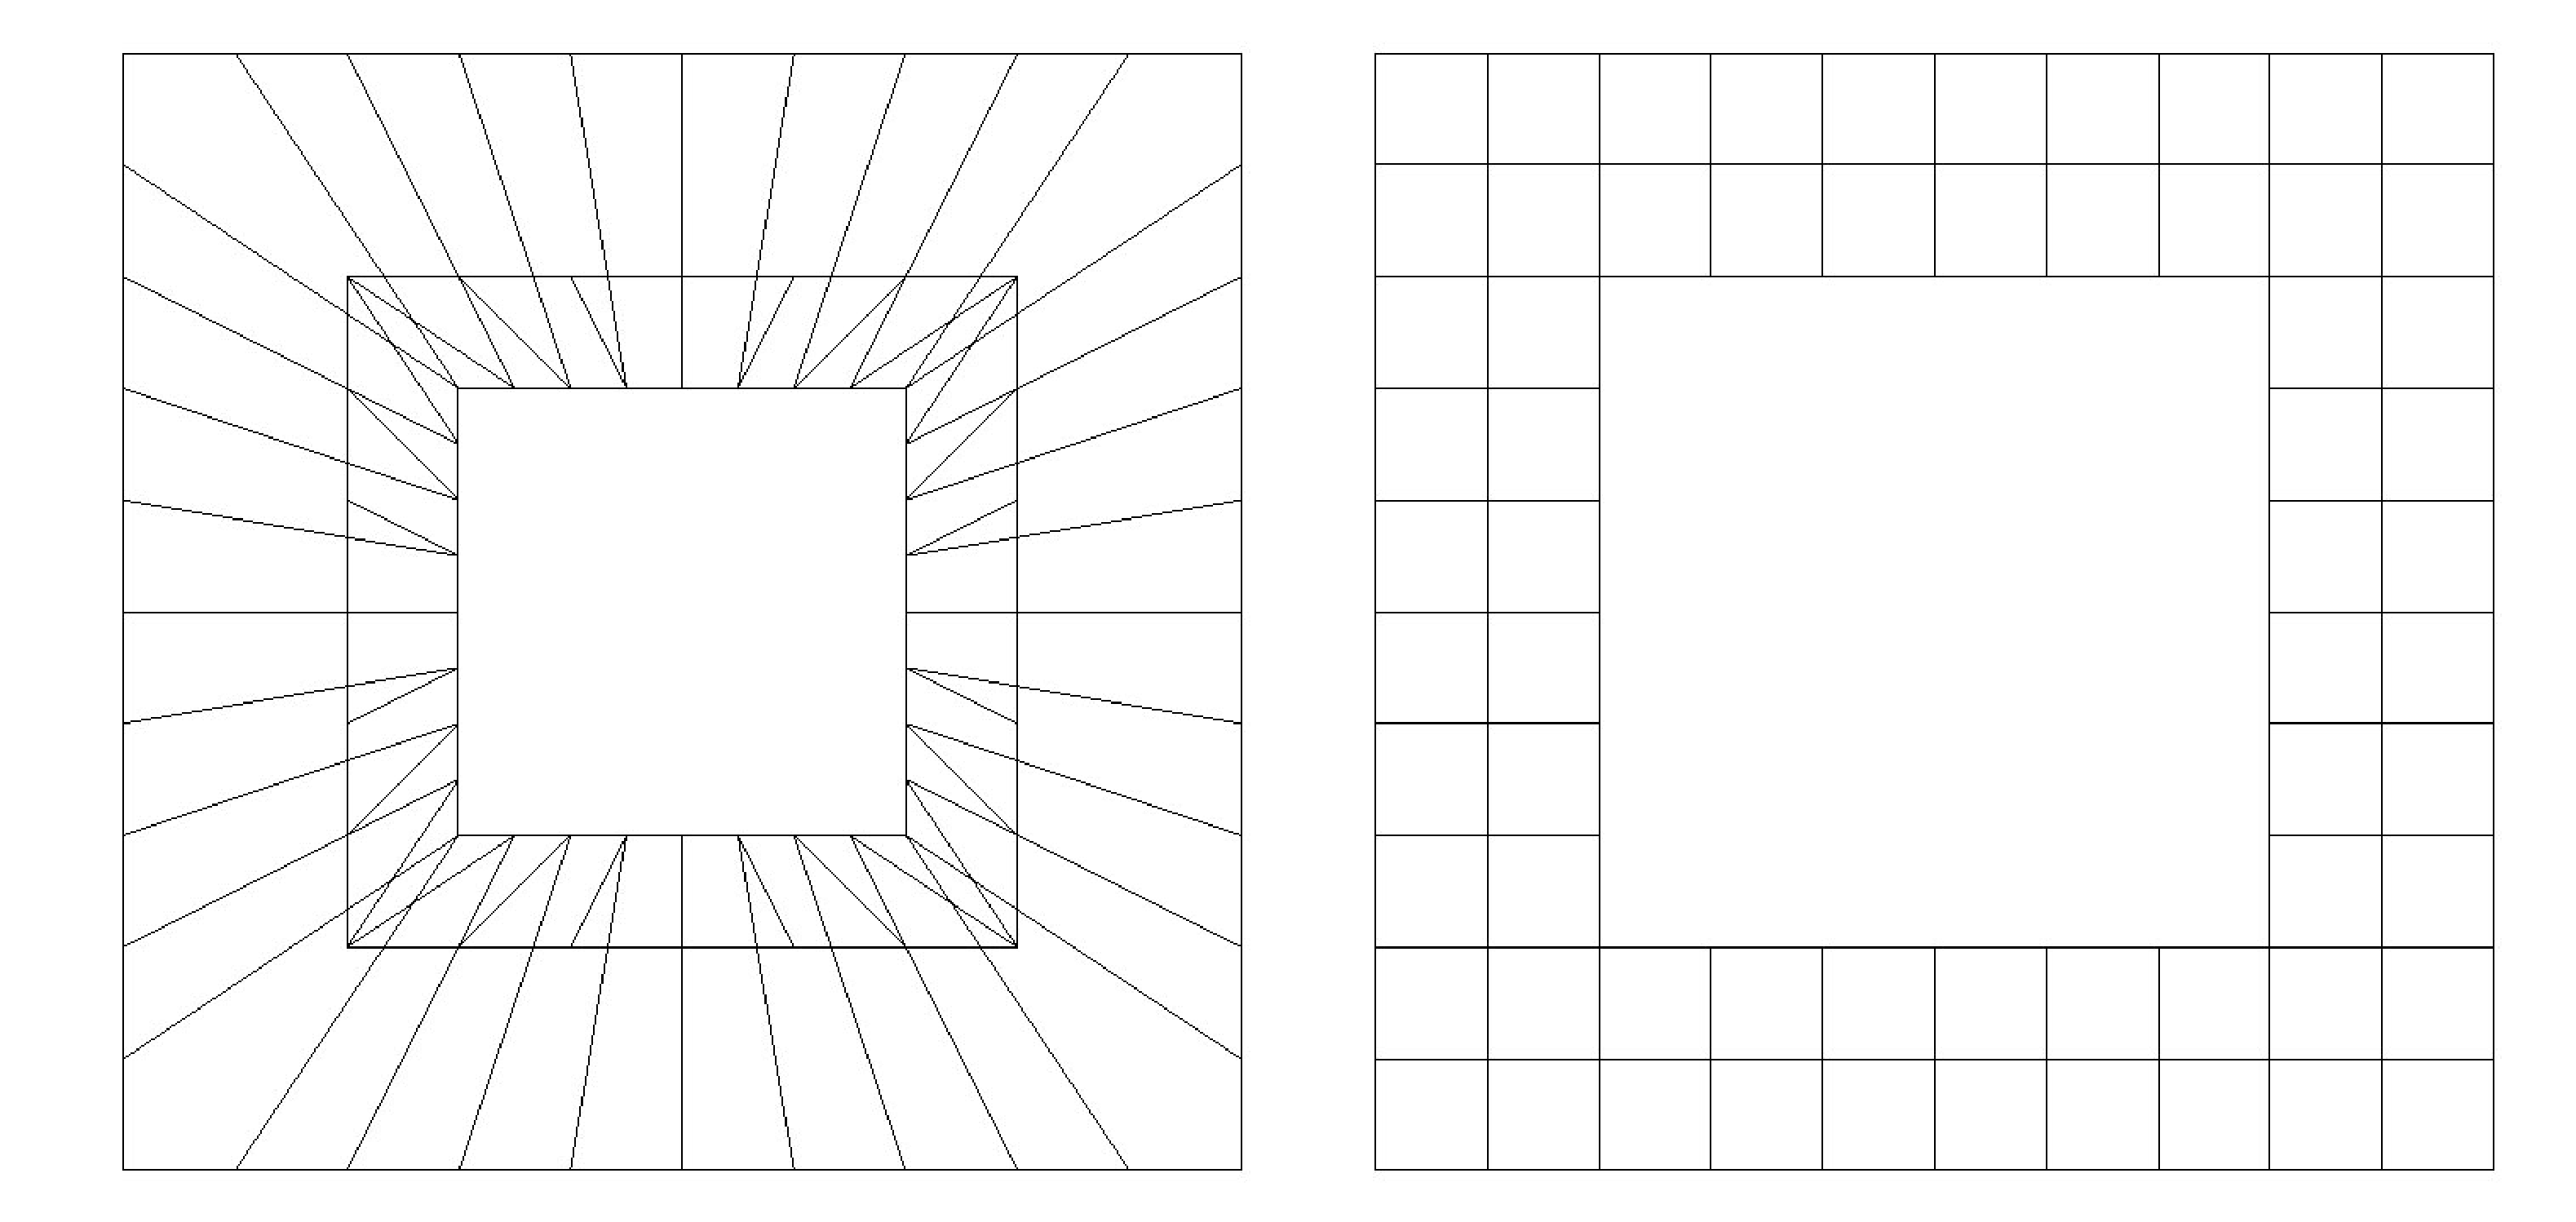
\includegraphics[height=75mm]{inverted-hole-1.eps}
    \caption{LaplaceWrapper, file: inverted-hole-1.vtk mesh. The original mesh is on the left, the mesh smoothed with the \texttt{LaplacianSmoother} is shown on the right.}
    \label{fig:inverted_hole_1}
\end{center}
\end{figure*}

\newpage

\section{Shape-Improvement} \label{sec:ShapeImprover}

\noindent {\it Name}: ShapeImprover \newline
\noindent {\it Purpose}: Make the shape of an element as close as possible to 
that of the ideal/regular element shape. For example, make triangular and 
tetrahedral elements equilateral.  The wrapper will use a non-barrier metric
until the mesh contains no inverted elements.  If the initial mesh was not tangled this phase will not modify the mesh.  If no limit is imposed on CPU
time or time remains a second phase using a barrier metric will further 
optimize the mesh with the guarantee that no elements will become inverted. \newline
\noindent {\it Notes}: Will return failure if mesh contains inverted elements after first phase.\newline
\noindent {\it Limitations/assumptions}:  \newline 
\noindent {\it Input Termination Criterion}: CPU time limit (not used if input 
value is non-positive) or fraction of mean edge length (default is 0.005). \newline \newline

\noindent Under the Cover: \newline
\noindent {\it Metric}: TMPQualityMetric(Shape/ShapeBarrier) \newline
\noindent {\it Objective Function}: Algebraic mean of quality metric values \newline
\noindent {\it Mesh/Element Type}: Any supported type. \newline
\noindent {\it Solver}: Conjugate Gradient \newline
\noindent {\it Global/Local}: Global \newline

\noindent Example: \newline

\begin{verbatim}
************** QualityAssessor(free only) Summary **************

  Evaluating quality for 40 elements.
  This mesh had 40 quadrilateral elements.
  There were no inverted elements detected. 
  No entities had undefined values for any computed metric.

                  metric     minimum     average         rms     maximum    std.dev.
 ElementPMeanP(TShapeB1)   0.0767863    0.232261    0.262717    0.404594    0.122781
ElementPMeanP(TShapeNB1)   0.0140953   0.0601601   0.0718989    0.118462   0.0393729
      Inverse Mean Ratio     1.07679     1.23226     1.23836     1.40459    0.122781

************** QualityAssessor(free only) Summary **************

  Evaluating quality for 40 elements.
  This mesh had 40 quadrilateral elements.
  There were no inverted elements detected. 
  No entities had undefined values for any computed metric.

                  metric     minimum     average         rms     maximum    std.dev.
 ElementPMeanP(TShapeB1)   0.0767863    0.232261    0.262717    0.404594    0.122781
ElementPMeanP(TShapeNB1)   0.0140953   0.0601601   0.0718989    0.118462   0.0393729
      Inverse Mean Ratio     1.07679     1.23226     1.23836     1.40459    0.122781

************** QualityAssessor(free only) Summary **************

  Evaluating quality for 40 elements.
  This mesh had 40 quadrilateral elements.
  There were no inverted elements detected. 
  No entities had undefined values for any computed metric.

                  metric     minimum     average         rms     maximum    std.dev.
 ElementPMeanP(TShapeB1)    0.121425      0.2041    0.207481    0.326159   0.0373025
ElementPMeanP(TShapeNB1)   0.0192667   0.0495255   0.0542939    0.101861   0.0222498
      Inverse Mean Ratio     1.12142      1.2041     1.20468     1.32616   0.0373025
\end{verbatim}

\begin{figure*}[htbp]
\begin{center}
    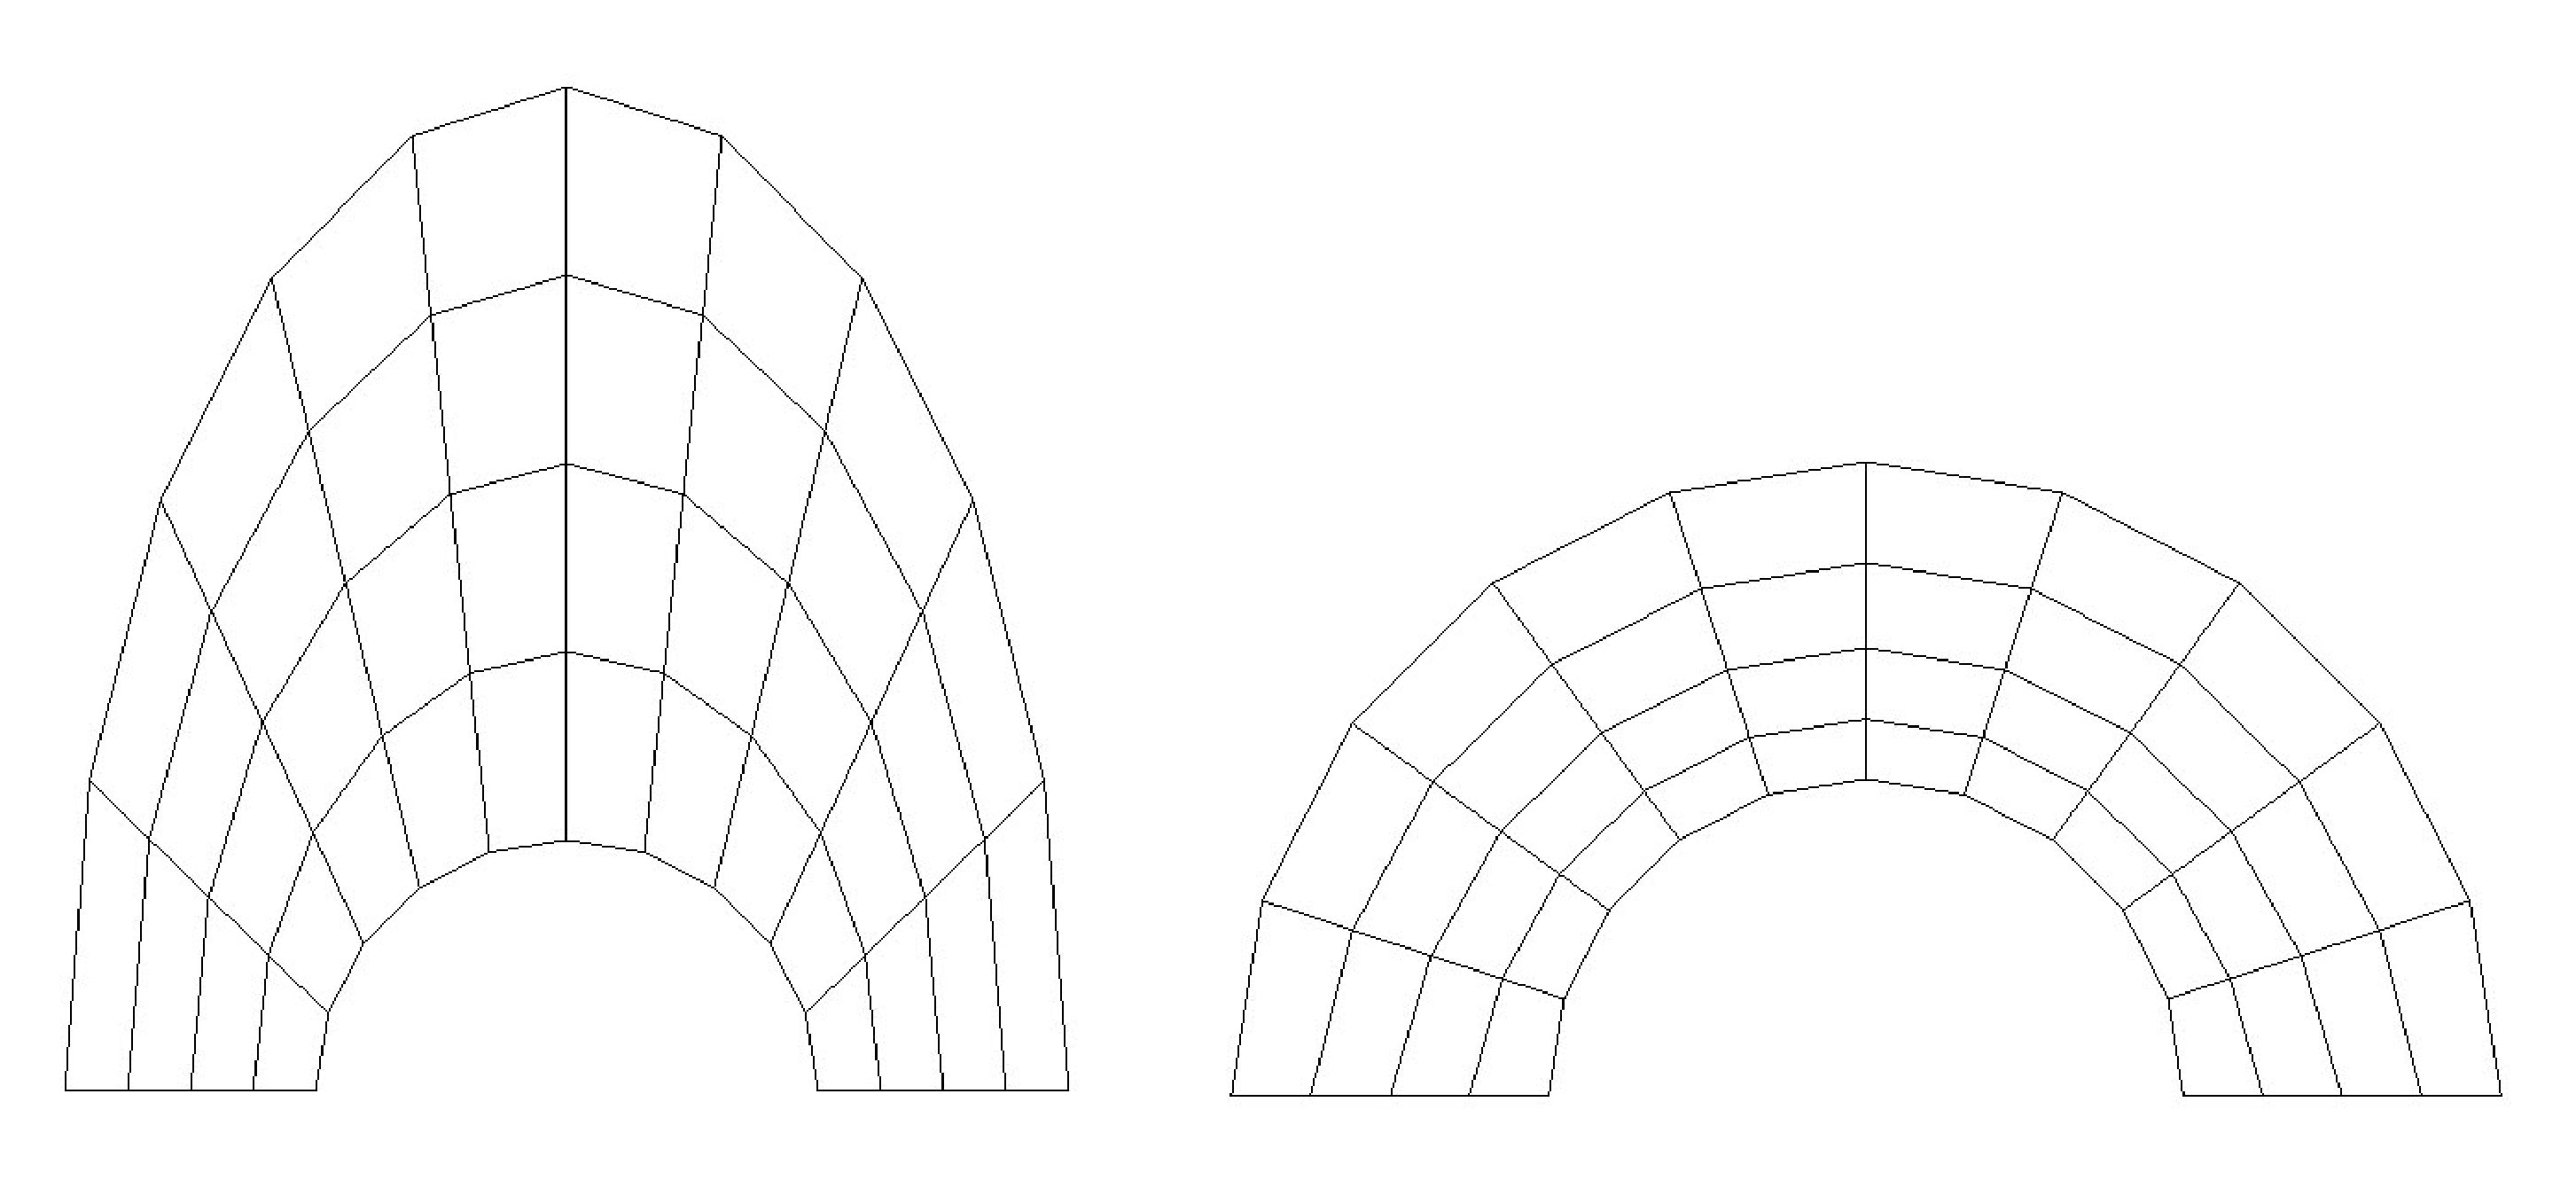
\includegraphics[height=80mm]{horseshoe-10x4.eps}
    \caption{ShapeImproverWrapper, file: tfi\_horse10x4-12.vtk mesh. The original mesh is on the left, the improved mesh is shown on the right.}
    \label{fig:inverted-hole-1}
\end{center}
\end{figure*}

\newpage

\section{Untangler} \label{sec:Untangler}

\noindent {\it Name}: UntangleWrapper \newline
\noindent {\it Purpose}: Untangle elements.  Prioritizes untangling over
element shape or other mesh quality measures.  \newline
\noindent {\it Notes}: A second optimization to improve element quality
after untangling is often necessary.  \newline
\noindent {\it Limitations/assumptions}: There is no guarantee that the optimal mesh computed using this wrapper will, in fact, be untangled.  \newline 
\noindent {\it Input Termination Criterion}: CPU time limit (not used if input 
value is non-positive) or fraction of mean edge length (default is 0.005).  It
also terminates if all elements are untangled, such that it should not modify
an input mesh with no inverted elements. \newline \newline

\noindent Under the Cover: \newline
\noindent {\it Metric}: TUntangleBeta or TUntangleMu(TSizeNB1) or TUntangleMu(TShapeSizeNB1) \newline
\noindent {\it Objective Function}: Algebraic mean of quality metric values \newline
\noindent {\it Mesh/Element Type}: Any supported type. \newline
\noindent {\it Solver}: Steepest Descent \newline
\noindent {\it Global/Local}: Local with culling, optionally Jacobi \newline

\noindent Example: \newline

\begin{verbatim}
**********************************************
Running "shest_grid32.vtk" for SHAPESIZE
**********************************************

************** QualityAssessor(free only) Summary **************

  Evaluating quality for 1024 elements.
  This mesh had 1024 quadrilateral elements.
  THERE ARE 9 INVERTED ELEMENTS.
  (Elements invalid at 9 of 4096 sample locations.)

  No entities had undefined values for any computed metric.

             metric     minimum     average         rms     maximum    std.dev.
ElementPMeanP(untangle(2D:TShapeSize2DNB1; 3D:TShapeSize3DNB1))
                              0     48.5379     210.965     2915.69     205.305

************** QualityAssessor(free only) Summary **************

  Evaluating quality for 1024 elements.
  This mesh had 1024 quadrilateral elements.
  There were no inverted elements detected.
  No entities had undefined values for any computed metric.

             metric     minimum     average         rms     maximum    std.dev.
ElementPMeanP(untangle(2D:TShapeSize2DNB1; 3D:TShapeSize3DNB1))
                              0     1.46636     23.8476     462.591     23.8025
\end{verbatim}


\begin{figure*}[htbp]
\begin{center}
    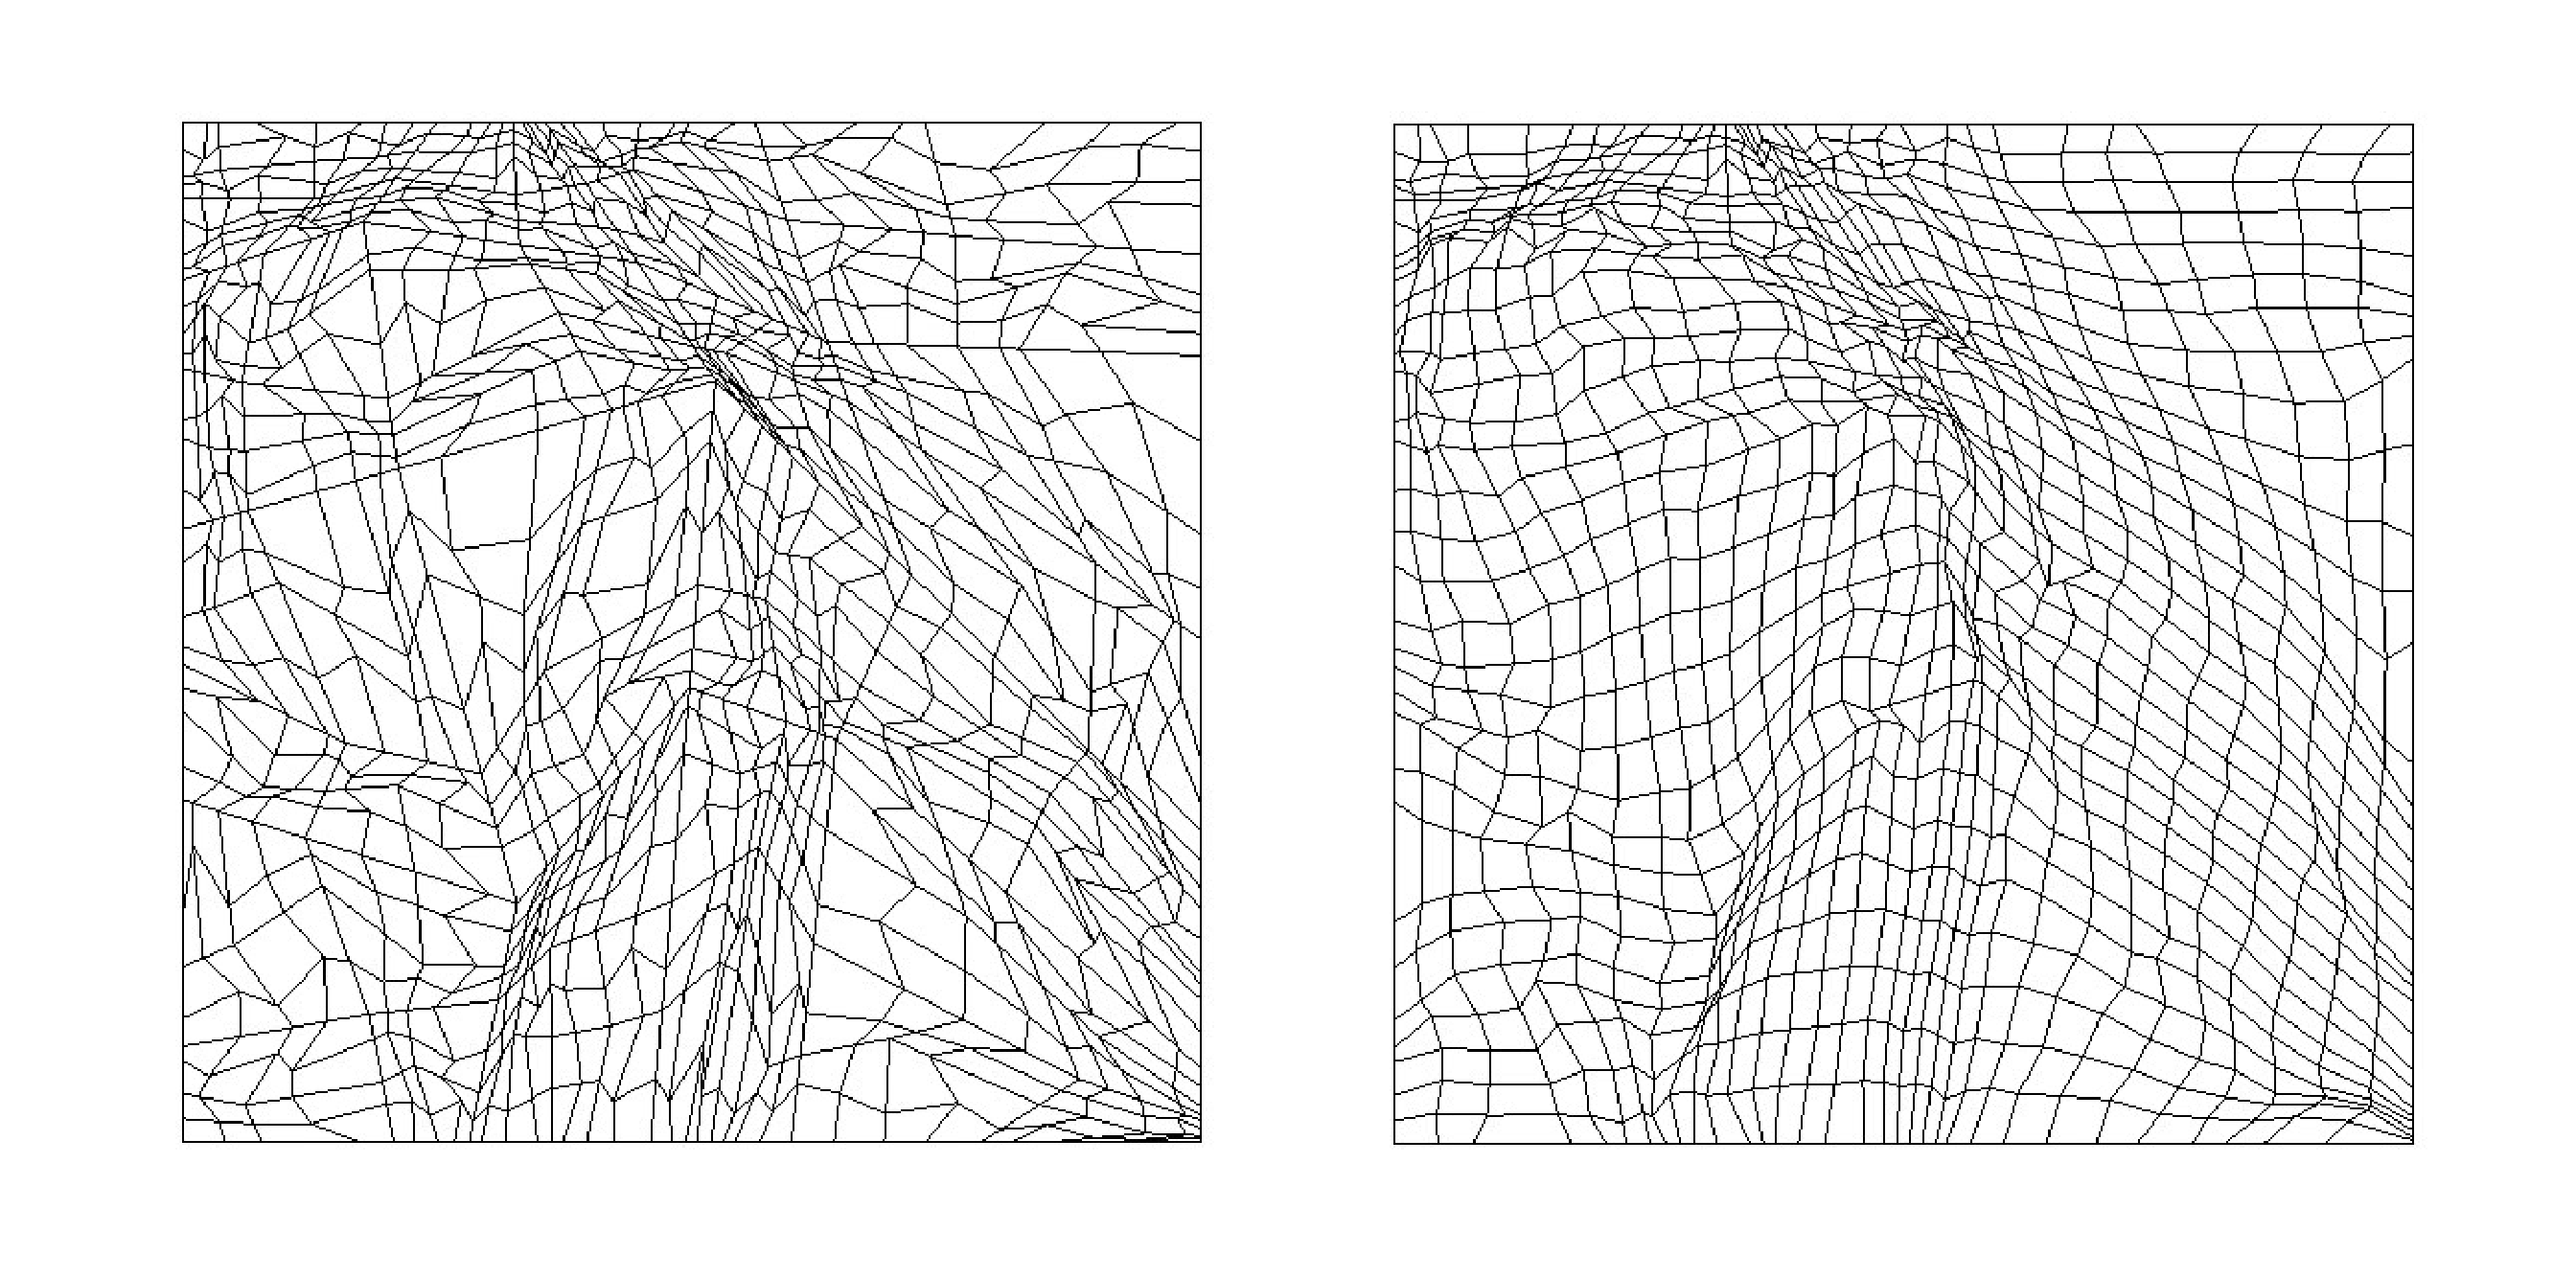
\includegraphics[height=80mm]{shest_grid32.eps}
    \caption{UntangleWrapper, TShapeSizeNB1 option, file: shest\_grid32.vtk mesh. The original mesh is on the left, the untangled mesh is shown on the right.}
    \label{fig:shest_grid32}
\end{center}
\end{figure*}

\newpage

\section{Minimum Edge-Length Improvement} \label{sec:PaverMinEdgeLengthWrapper}

\noindent {\it Name}: PaverMinEdgeLengthWrapper \newline
\noindent {\it Purpose}: Make all the edges in the mesh of equal length while 
moving toward the ideal shape. Intended for explicit PDE codes whose 
time-step limination is governed by the minimum edge-length in the mesh. \newline
\noindent {\it Notes}: Based on Target-matrix paradigm. \newline
\noindent {\it Limitations/assumptions}: Initial mesh must be non-inverted. User does not want to preserve or create anisotropic elements. \newline 
\noindent {\it Input Termination Criterion}: maximum iterations (default=50), maximum absolute vertex movement \newline \newline

\noindent Under the Cover: \newline
\noindent {\it Hardwired Parameters}: None \newline
\noindent {\it Metric}:  Target2DShapeSizeBarrier or Target3DShapeSizeBarrier \newline
\noindent {\it Tradeoff Coefficient}: 1.0 \newline
\noindent {\it Objective Function}: Linear Average over the Sample Points \newline
\noindent {\it Mesh/Element Type}: Any supported type.  \newline
\noindent {\it Solver}: Trust Region \newline
\noindent {\it Global/Local}: Global \newline

\noindent Example: \newline

\begin{verbatim}
************** QualityAssessor(free only) Summary **************

  Evaluating quality for 8 elements.
  This mesh had 8 quadrilateral elements.
  There were no inverted elements detected. 
  No entities had undefined values for any computed metric.

                     metric     minimum     average         rms     maximum    std.dev.
ElementPMeanP(TShapeSizeB1)    0.357275    0.983461     1.33806     3.27555    0.907303
                 EdgeLength    0.538516     1.11317     1.15398     1.51327    0.304184

************** QualityAssessor(free only) Summary **************

  Evaluating quality for 8 elements.
  This mesh had 8 quadrilateral elements.
  There were no inverted elements detected. 
  No entities had undefined values for any computed metric.

                     metric     minimum     average         rms     maximum    std.dev.
ElementPMeanP(TShapeSizeB1)  0.00135009   0.0017804  0.00179488  0.00221721 0.000227498
                 EdgeLength    0.994086      1.0004     1.00041     1.00293  0.00253389
\end{verbatim}


\begin{figure*}[htbp]
\begin{center}
    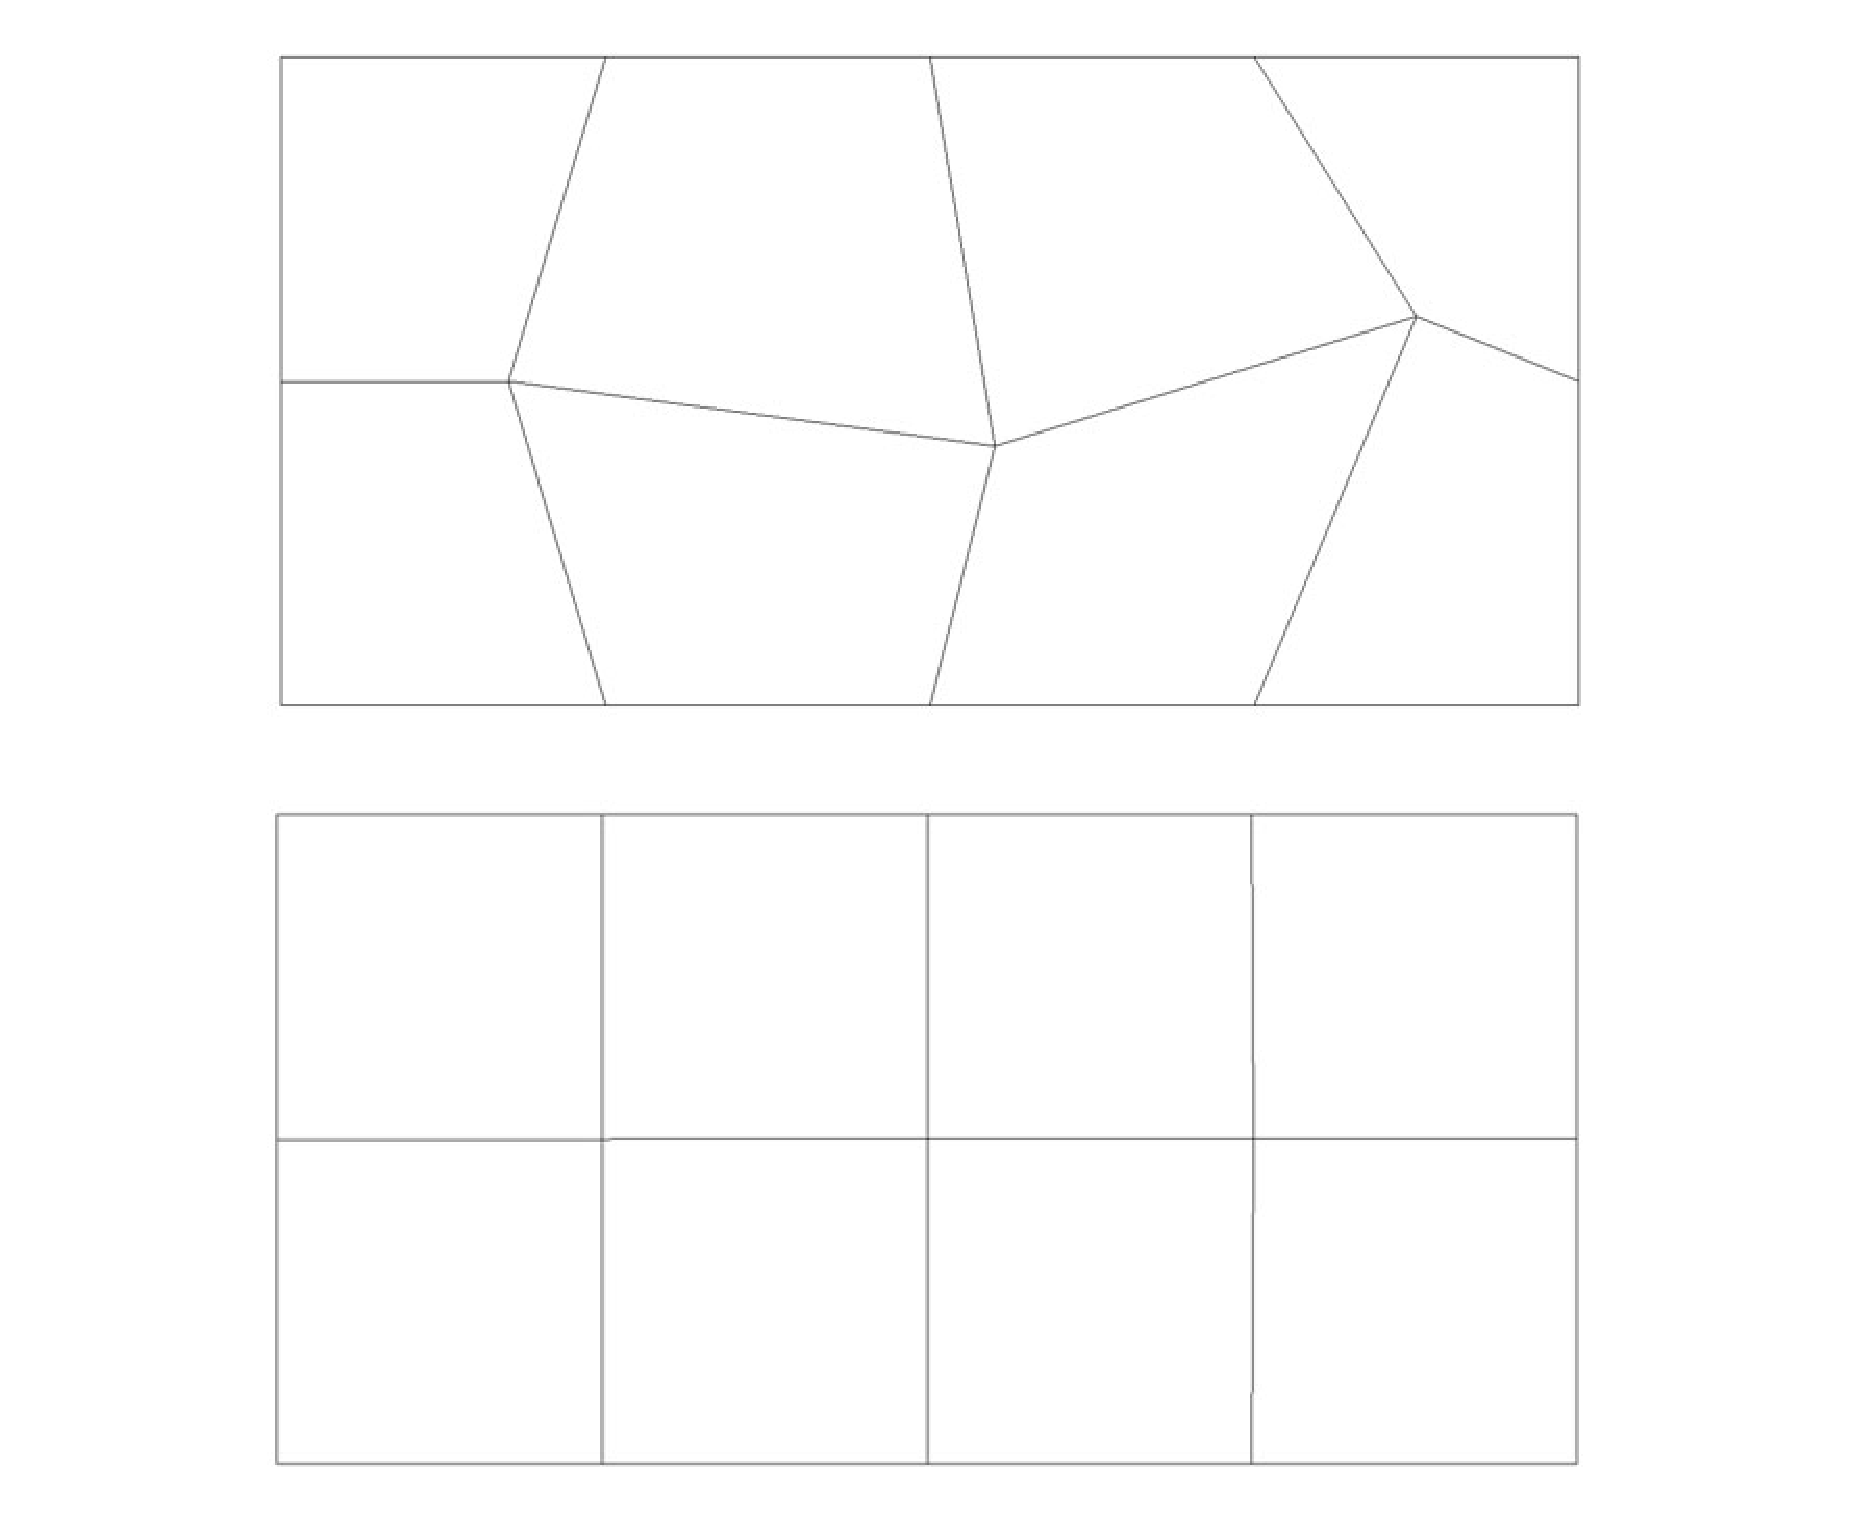
\includegraphics[height=100mm]{min-edge-length.eps}
    \caption{PaverMinEdgeLengthWrapper, file: quads\_4by2\_bad.vtk mesh. The original mesh is on the top, the improved mesh is shown on the bottom.}
    \label{fig:min_edge-length}
\end{center}
\end{figure*}
 
\newpage

\section{Improve the Shapes in a Size-adapted Mesh} \label{sec:SizeAdaptShapeWrapper}

\noindent {\it Name}: SizeAdaptShapeWrapper \newline
\noindent {\it Purpose}: Make the shape of an element as close as possible to that
of the ideal element shape, {\it while preserving, as much as possible, the size of each element in the mesh}. To be used on isotropic initial meshes that are already size-adapted. \newline
\noindent {\it Notes}: Based on Target-matrix Paradigm. \newline
\noindent {\it Limitations/assumptions}: Initial mesh must be non-inverted. 
User wants to preserve sizes of elements in initial mesh and does not want to preserve or 
create anisotropic elements.  \newline 
\noindent {\it Input Termination Criterion}: maximum iterations (default=50), maximum absolute vertex movement \newline \newline

\noindent Under the Cover: \newline
\noindent {\it Hardwired Parameters}: None \newline
\noindent {\it Metric}: Target2DShapeSizeBarrier or Target3DShapeSizeBarrier \newline
\noindent {\it Tradeoff Coefficient}: 1.0 \newline
\noindent {\it Objective Function}: Linear Average over the Sample Points \newline
\noindent {\it Mesh/Element Type}: Any supported type. \newline
\noindent {\it Solver}: Trust Region \newline
\noindent {\it Global/Local}: Global \newline

\noindent Example: \newline

\begin{verbatim}
************** QualityAssessor(free only) Summary **************

  Evaluating quality for 3456 elements.
  This mesh had 3456 quadrilateral elements.
  There were no inverted elements detectedas-sphere-quads. 
  No entities had undefined values for any computed metric.

                     metric     minimum     average         rms     maximum    std.dev.
ElementPMeanP(TShapeSizeB1)  0.00447499     0.23505    0.288066    0.710249    0.166533
                 EdgeLength    0.163072    0.574857     0.62062     1.01908      0.2339


************** QualityAssessor(free only) Summary **************

  Evaluating quality for 3456 elements.
  This mesh had 3456 quadrilateral elements.
  There were no inverted elements detected. 
  No entities had undefined values for any computed metric.

                     metric     minimum     average         rms     maximum    std.dev.
ElementPMeanP(TShapeSizeB1)  0.00558463   0.0591772   0.0767815    0.303106    0.048923
                 EdgeLength    0.161144    0.562074    0.607611     1.11686    0.230789


AREAS:      Initial     Final       Difference  Change
Polar:
  Minimum:    0.035147    0.033739    0.001407    4.003825%
  Average:    0.356401    0.355561    0.000840    0.235642%
  Maximum:    0.956929    0.896340    0.060589    6.331607%
Equatorial:
  Minimum:    0.530028    0.650497    0.120469   22.728869%
  Average:    0.718328    0.763170    0.044842    6.242616%
  Maximum:    0.957685    0.896794    0.060891    6.358101%
\end{verbatim}


\begin{figure*}[htbp]
\begin{center}
    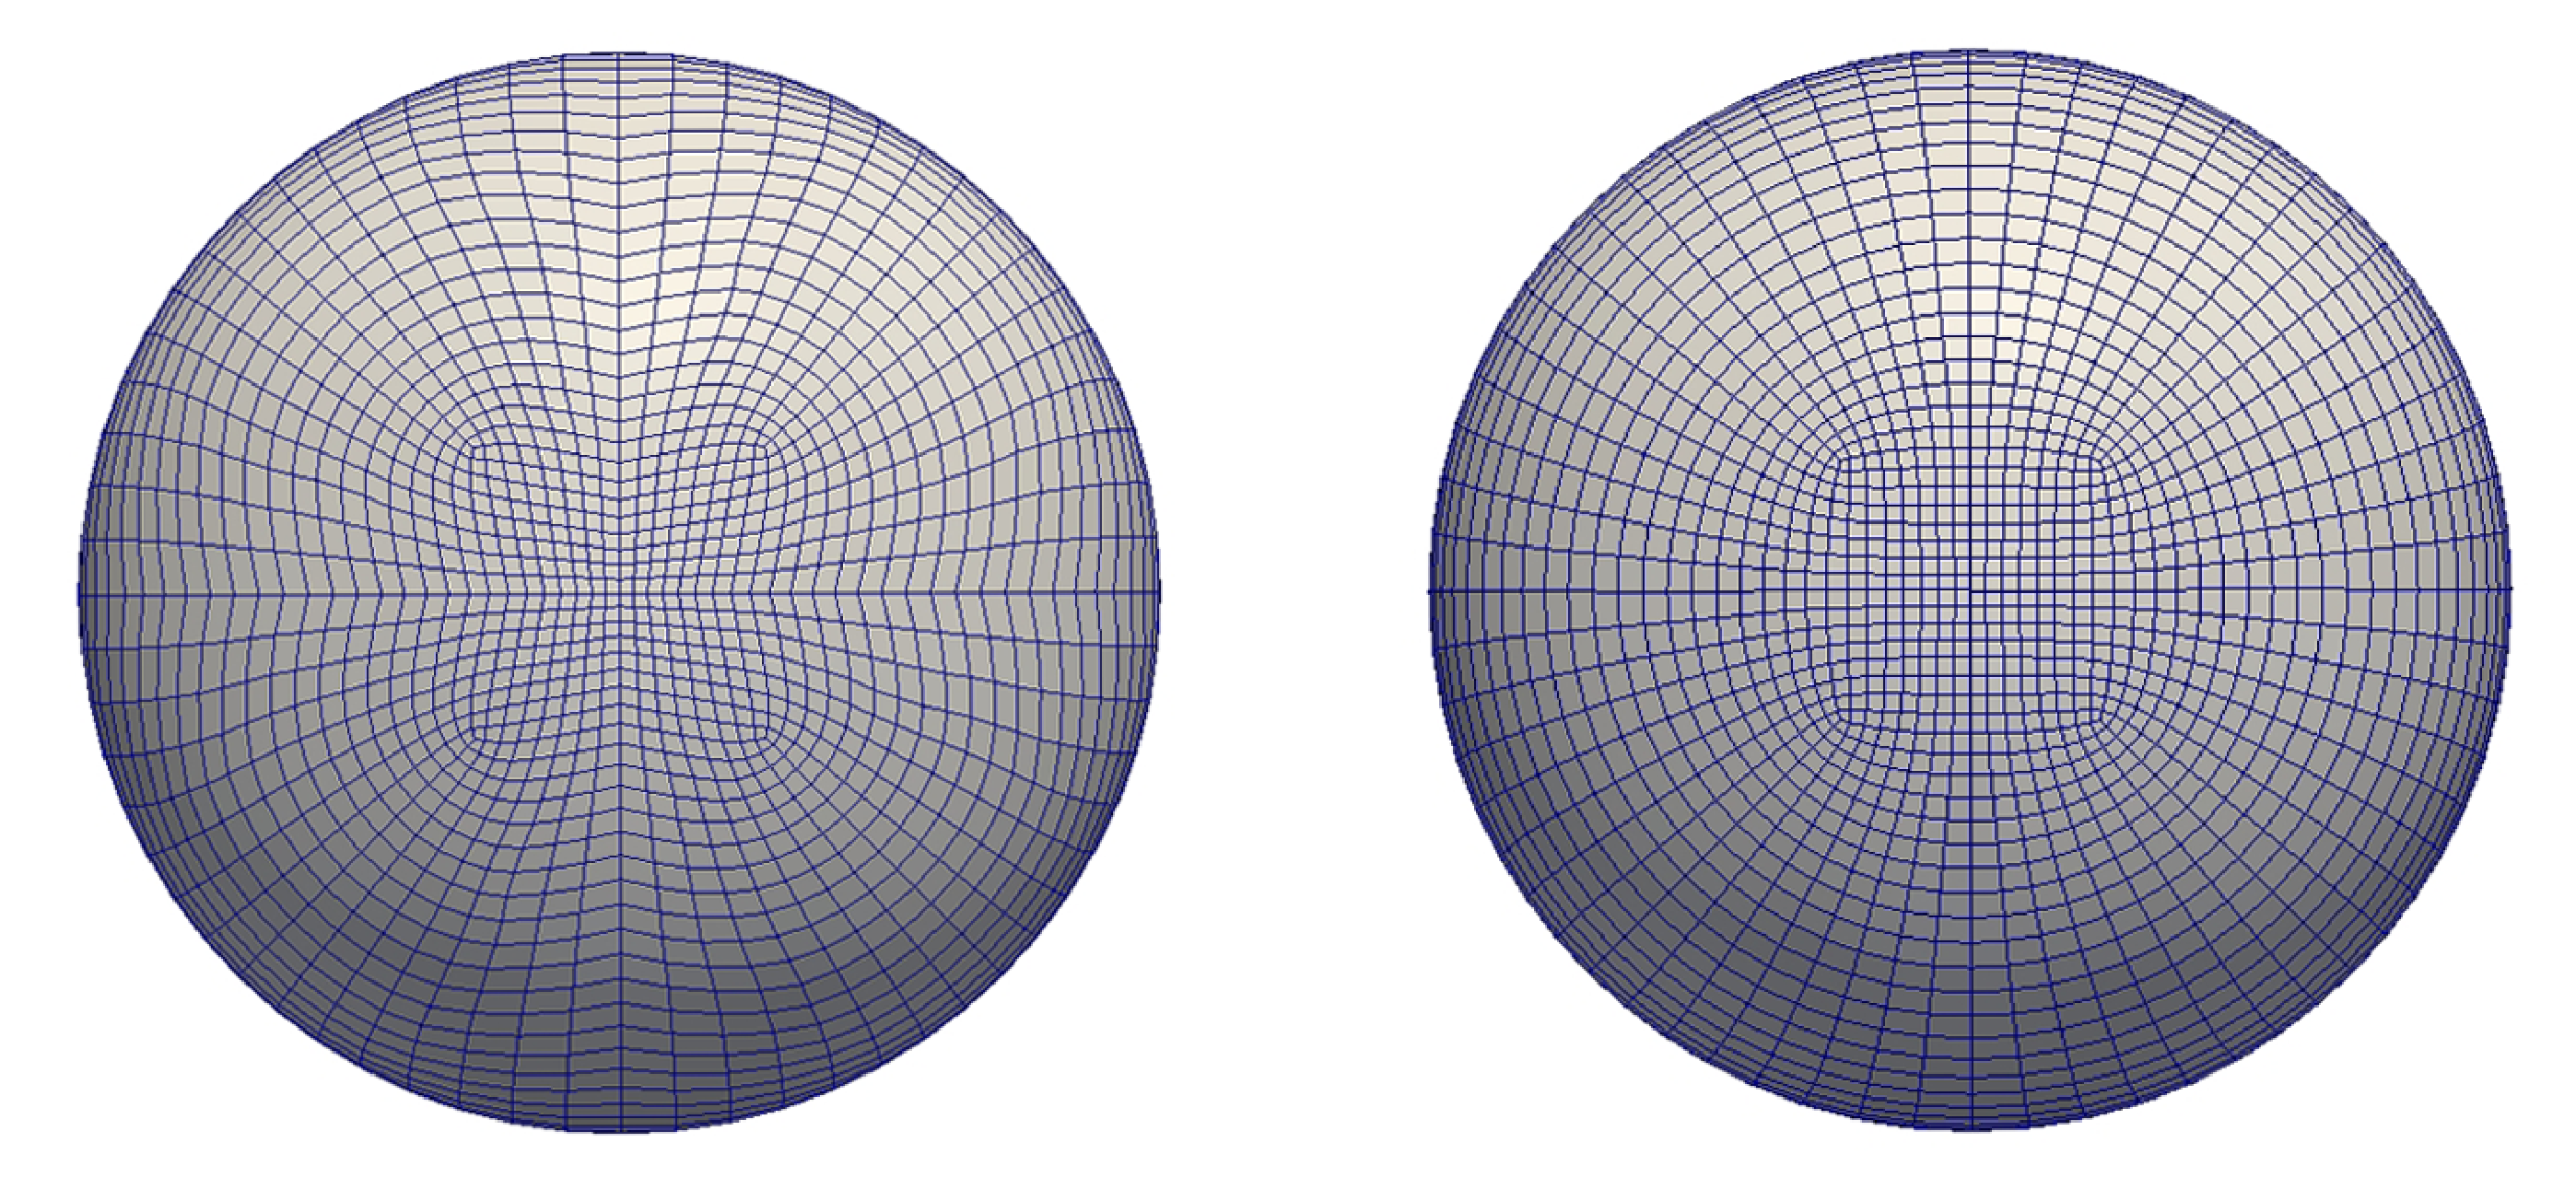
\includegraphics[height=80mm]{bias-sphere-quads.eps}
    \caption{SizeAdaptShapeWrapper, file: bias-sphere-quads.vtk mesh. The original mesh is on the left, the improved mesh is shown on the right.}
    \label{fig:shest_grid32}
\end{center}
\end{figure*}

\newpage

\section{Improve Sliver Tets in a Viscous CFD Mesh} \label{sec:ViscousCFDTetShapeWrapper}

\noindent {\it Name}: ViscousCFDTetShapeWrapper \newline
\noindent {\it Purpose}: Improve the shape of sliver elements in the far-field 
of a CFD mesh while 
preserving an existing layer of sliver elements in the boundary layer. \newline
\noindent Notes: Based on Target-matrix paradigm.  \newline
\noindent {\it Limitations/assumptions}: Tetrahedral meshes only.  \newline 
\noindent {\it Input Termination Criterion}: Iteration Count (default=50) or Maximum Absolution Vertex Movement \newline \newline
 
\noindent Under the Cover: \newline
\noindent {\it Hardwired Parameters}: In tradeoff coefficient model. \newline
\noindent {\it Metric}: Target2DShape+Target2DShapeSizeOrient (or 3D) (or Barrier) \newline
\noindent {\it Tradeoff Coefficient}: Based on element dihedral angle \newline
\noindent {\it Objective Function}: Linear average over Sample Points \newline
\noindent {\it Mesh/Element Type}: Tetrahedra \newline
\noindent {\it Solver}: Trust Region \newline
\noindent {\it Global/Local}: Global \newline


\noindent Additional Information: \newline
\noindent {\it Article}: Introducing the Target-matrix Paradigm for mesh optimization via node-movement", Engineering with Computers, Sept. 2011.\newline

\section{Deforming Domain} \label{sec:DeformingDomain}

\noindent {\it Name}: DeformingDomainWrapper \newline
\noindent {\it Purpose}:  Use initial mesh on undeformed geometric domain
to guide optimization of mesh moved to deformed geometric domain.  \newline
\noindent {\it Notes}: Uses a non-barrier metric which means that the
wrapper could potentially invert/tangle elements.  \newline
\noindent {\it Limitations/assumptions}:  Application responsible for explicit handling of mesh on geometric curves and points.  Initial mesh before moving to deformed domain must be available.\newline 
\noindent {\it Input Termination Criterion}: CPU time limit (not used if input 
value is non-positive) or fraction of mean edge length (default is 0.005). \newline \newline

\noindent Under the Cover: \newline
\noindent {\it Metric}: TMPQualityMetric(TShapeNB1 or TShapeSizeNB1 or TShapeSizeOrientNB1) \newline
\noindent {\it Objective Function}: Algebraic mean of quality metric values \newline
\noindent {\it Mesh/Element Type}: Any supported type. \newline
\noindent {\it Solver}: Steepest Descent \newline
\noindent {\it Global/Local}: Local with culling \newline

\noindent Additional Information: \newline
\noindent {\it Article}: "Updating meshes on deforming domains",  Communications in Numerical Methods in Engineering, 24:467-476, 2008..\newline

\noindent Example: \newline

\begin{verbatim}
************** QualityAssessor(free only) Summary **************

  Evaluating quality for 216 elements.
  This mesh had 216 quadrilateral elements.
  THERE ARE 56 INVERTED ELEMENTS. 
  (Elements invalid at 220 of 864 sample locations.)

  No entities had undefined values for any computed metric.

                  metric     minimum     average         rms     maximum    std.dev.
ElementPMeanP(TShapeNB1) 4.57621e-05     7.63416     20.8252     67.0217     19.3754

************** QualityAssessor(free only) Summary **************

  Evaluating quality for 216 elements.
  This mesh had 216 quadrilateral elements.
  There were no inverted elements detected. 
  No entities had undefined values for any computed metric.

                  metric     minimum     average         rms     maximum    std.dev.
ElementPMeanP(TShapeNB1) 0.000763758   0.0202682   0.0252805   0.0947676   0.0151097
\end{verbatim}


\begin{figure*}[htbp]
\begin{center}
    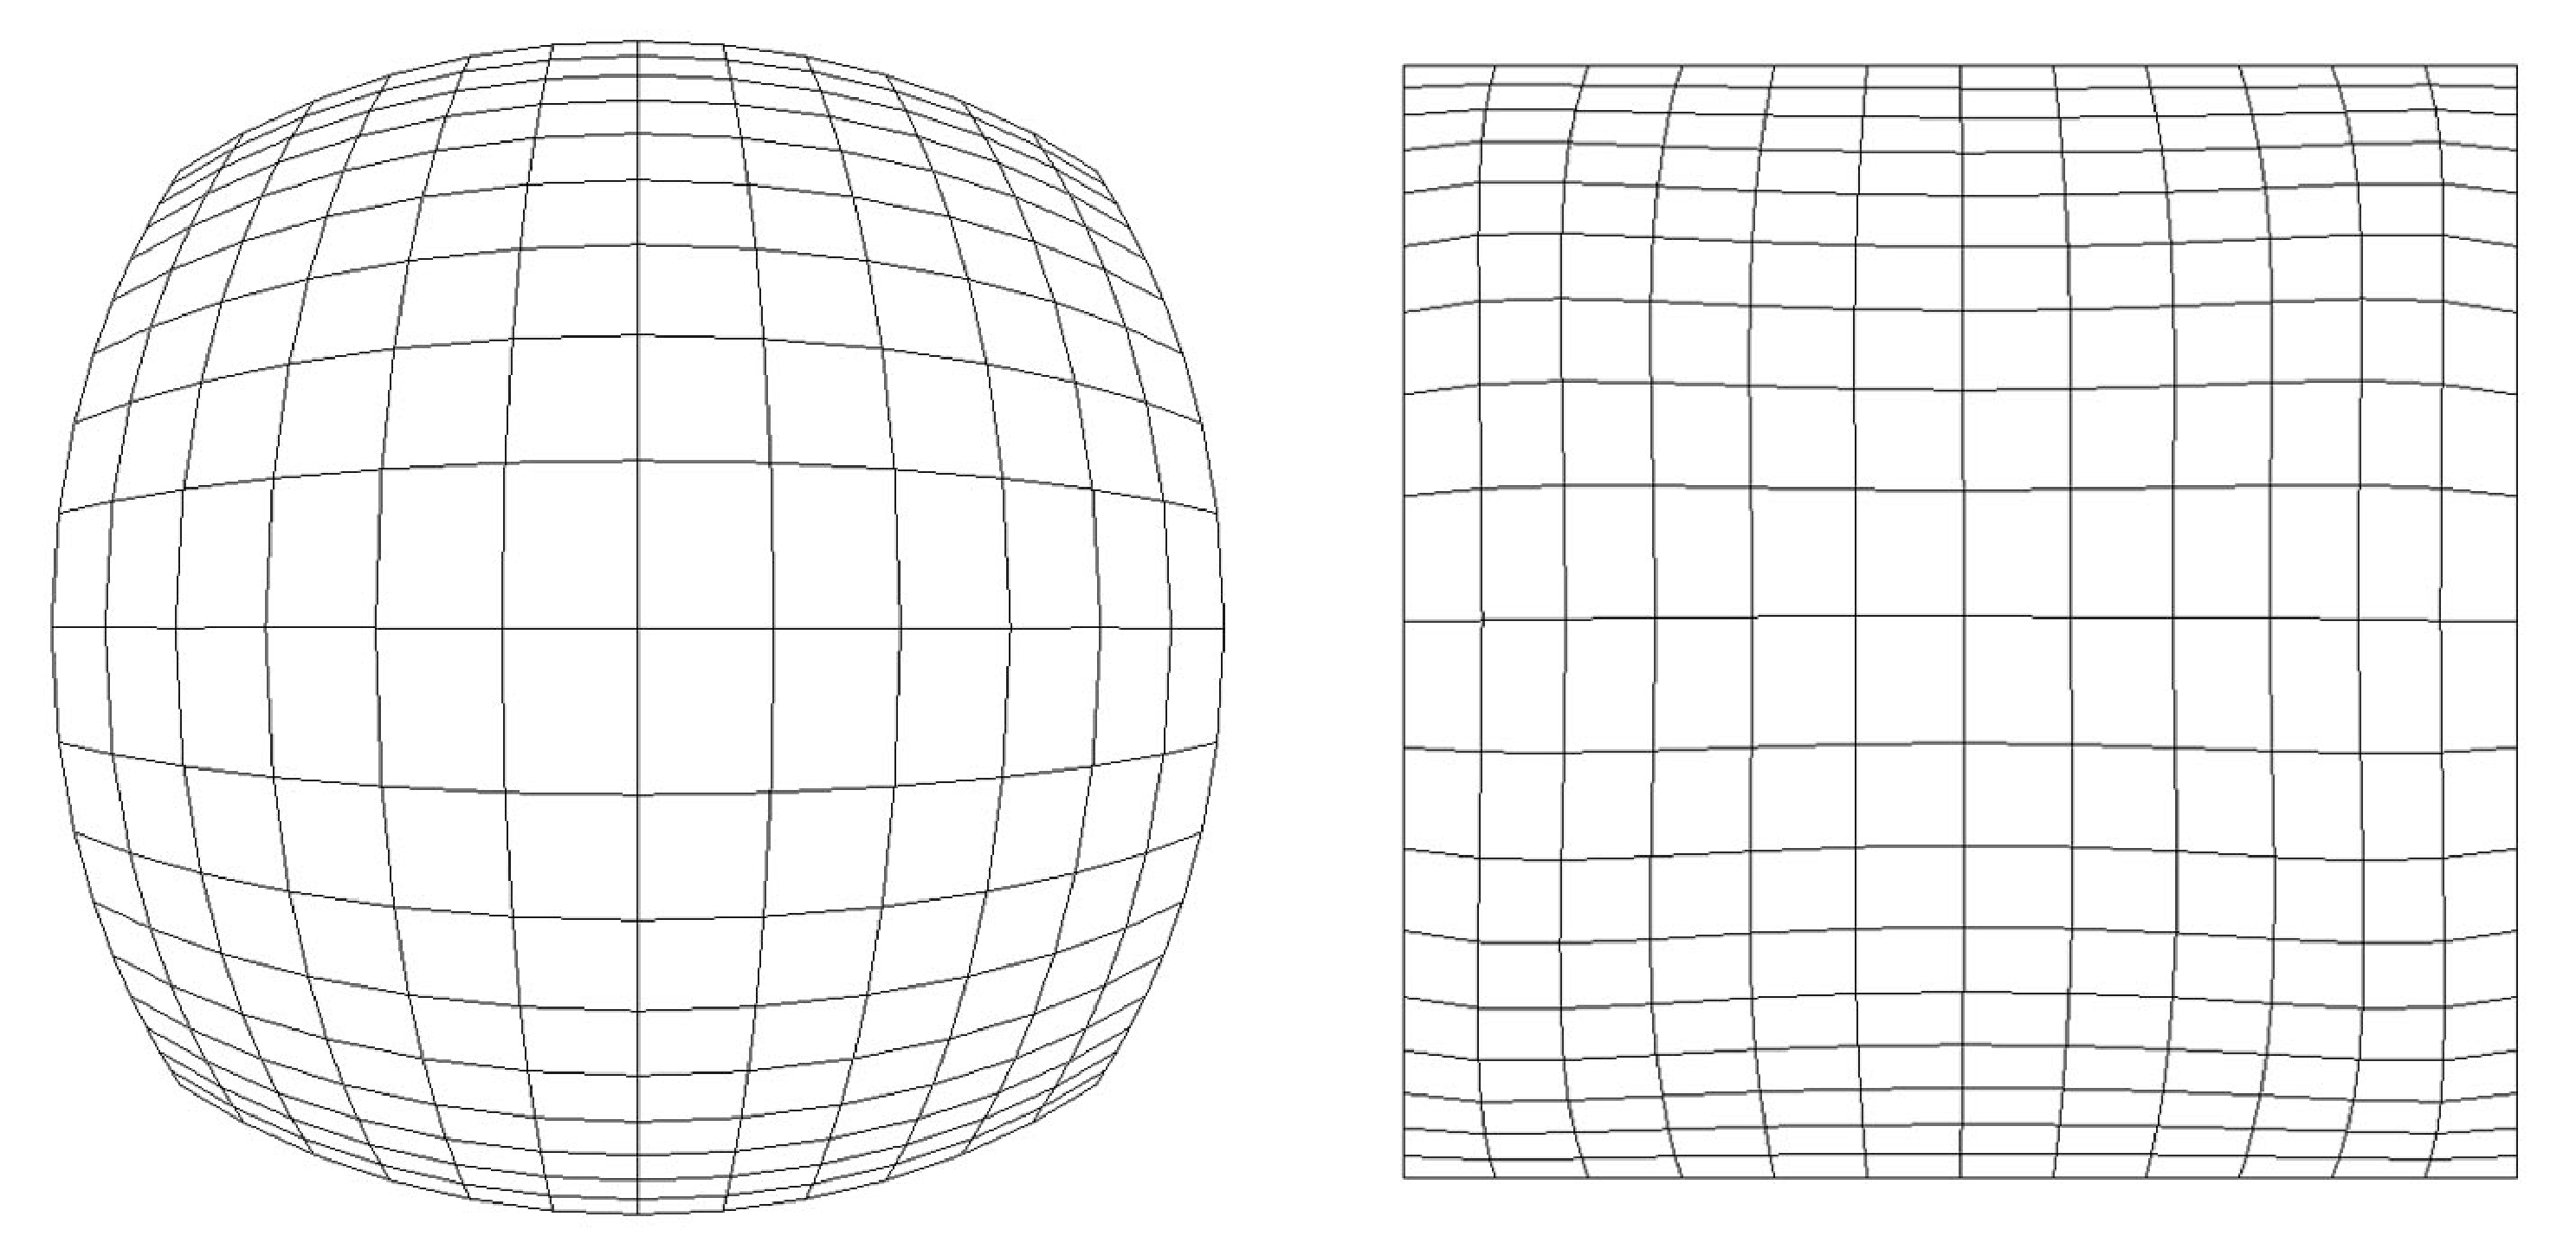
\includegraphics[height=80mm]{sph-10-zsquare.eps}
    \caption{DeformingDomainWrapper, file: sph-10-zsquare.vtk mesh. The original mesh is on the left, the improved mesh is shown on the right.}
    \label{fig:sph-10-zsquare}
\end{center}
\end{figure*}


% Optimization strategies (Nash, global, culling, etc.)
\chapter{Optimization Strategies \label{ch:optstrat}}

\section{The Generalized Optimization Loop}

In Mesquite a generalization of the optimization strategy is used to implement a wide variety of optimization strategies.  Before discussing the different types of optimization strategies that can be implemented with Mesquite we will first need to discuss the generalized strategy.

The mesh can be decomposed into subsets called {\em patches}.  The specifics of this mesh decomposition are discussed in Section \ref{sec:patches}.  The optimization is done by repeatedly iterating over the set of patches, optimizing each separately.

\begin{figure}[htb!]
\begin{center}
\noindent\makebox[\textwidth]{%
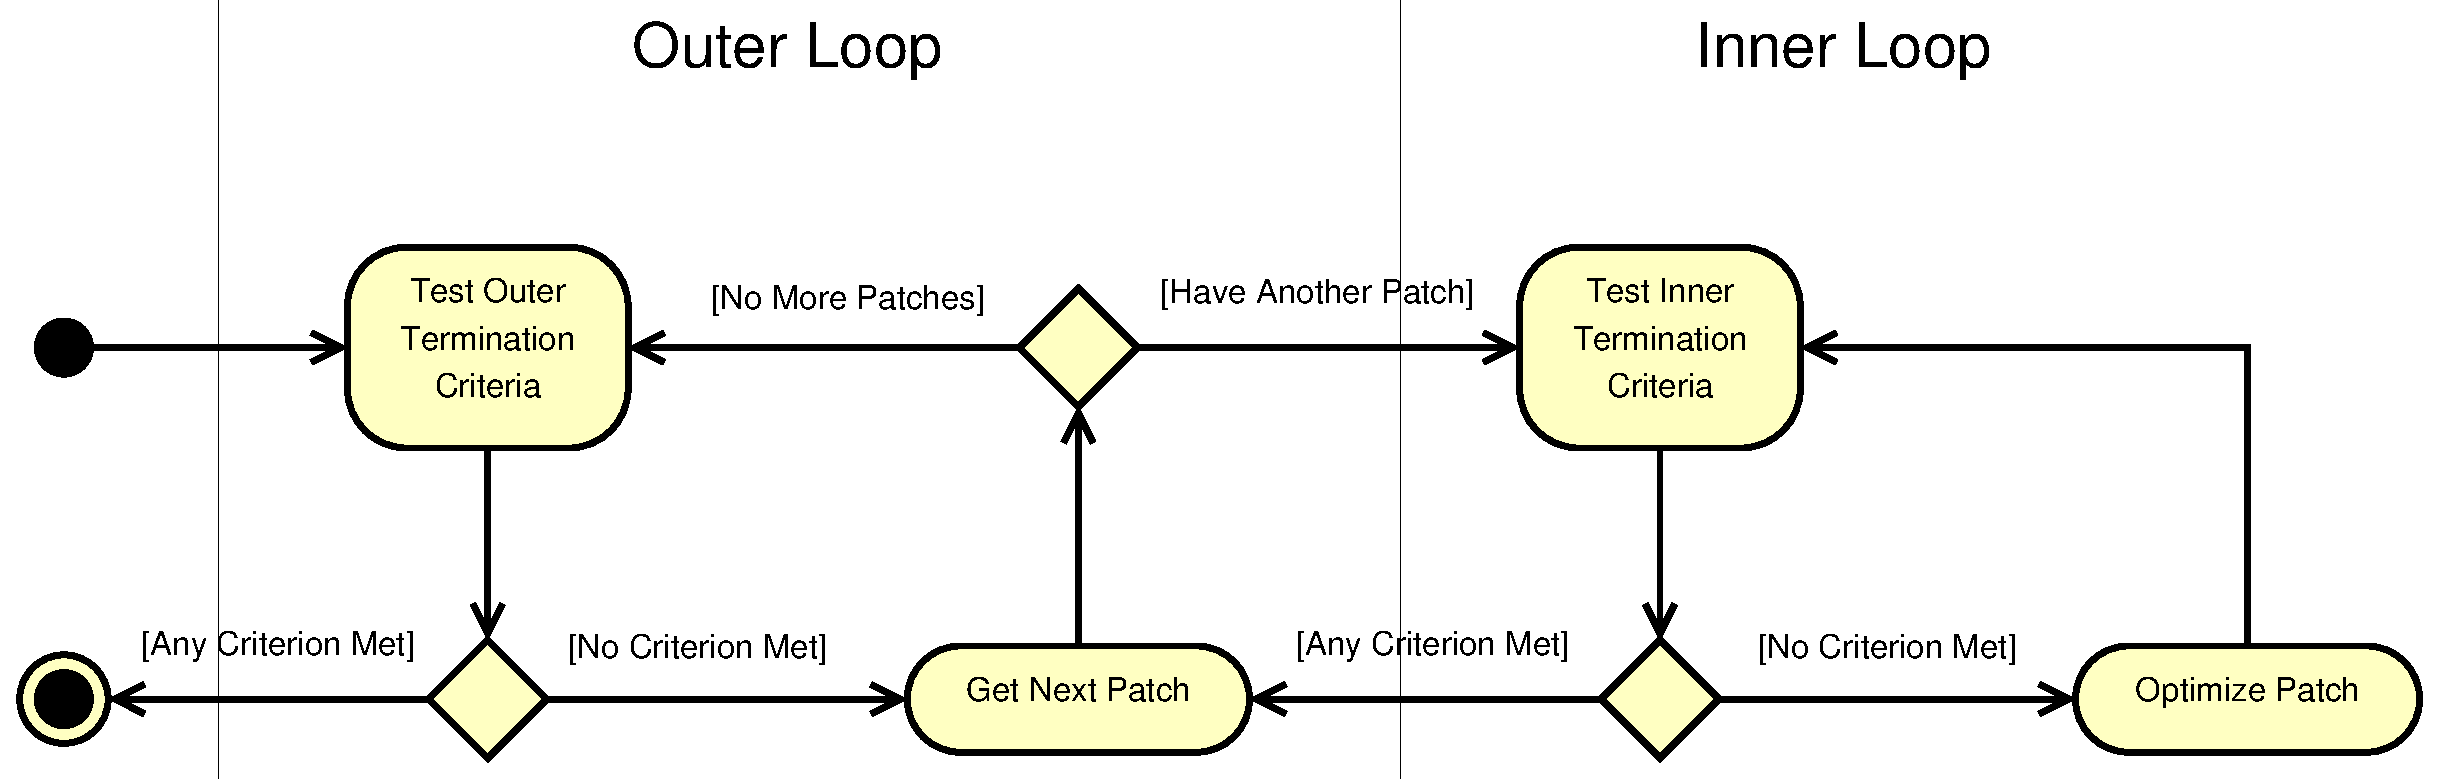
\includegraphics[width=6.5in]{generalized_optimization}}
\caption{\em Optimization Loop \label{fig:genoptloop}}
\end{center}
\end{figure}

Figure \ref{fig:genoptloop} depicts the generalization of optimization strategies in Mesquite.  The generalized optimization is composed of three loops shown as non-overlapping square cycles in the diagram.  The test to exit each loop is performed at the decision points (diamonds) in the diagram.  The loops are logically nested from left to right, such that the right most loop is performed within a single iteration of the loop to the left of it.  The inner- and outer-most loops terminate based on user-definable termination criterion.  The center loop is the iteration over the set of patches composing the mesh.

The inner-most loop (the right-most cycle in the diagram) represents the iterative optimization of the mesh contained in a single patch.  This optimization is done until the {\em inner termination criterion} is met.  Once the inner criterion is met the optimizer advances to the next patch and the inner loop is entered again to optimize that patch.  Once each patch has been optimized the {\em outer termination criterion} is tested.  If the criterion has not been met then the loop over the set of patches is repeated.

The set of outer termination criteria determine when the optimization of the entire mesh is complete.  The set of inner termination criteria determine when the optimization of a single patch is complete.  Both sets of criteria are tested before entering their respective loops.  If a criterion is met before the loop starts then no iterations of the corresponding loop will be performed.

The outer loop(s) are implemented in the {\texttt VertexMover} class.  The inner loop is implemented in subclasses.  The {\texttt LaplacianSmoother} class in Mesquite provides a traditional Laplace smoother.  For this class the mesh is decomposed into patches that each contain a single free vertex and the adjacent elements, one patch for each free vertex in the mesh.  For Laplace smoothing the inner (per-vertex) optimization is not iterative.  The inner loop always has an implicit termination criterion of a single iteration.  Any other inner termination criterion will still be tested before performing the relaxation of the free vertex in the patch such that if any such criterion is met no optimization of the vertex will be performed.  However, culling (Section \ref{sec:culling} can have a similar effect while typically producing better results.  Passes are made over the entire mesh until one of the specified outer termination criterion is met.

\section{Patches \label{sec:patches}}


Mesquite can operate on a decomposition of the mesh into subsets called {\em patches}.  Each patch is optimized individually.  The overall mesh optimization is performed by repeatedly iterating over the set of patches.  Mesquite provides two build-in mesh decompositions\footnote{Mesquite includes an additional decomposition of the mesh into single-element patches which is not suitable for use in optimization.  It is used internally for quality assessment and other purposes}: element-on-vertex patches and a global patch.  

\begin{figure}[htb]
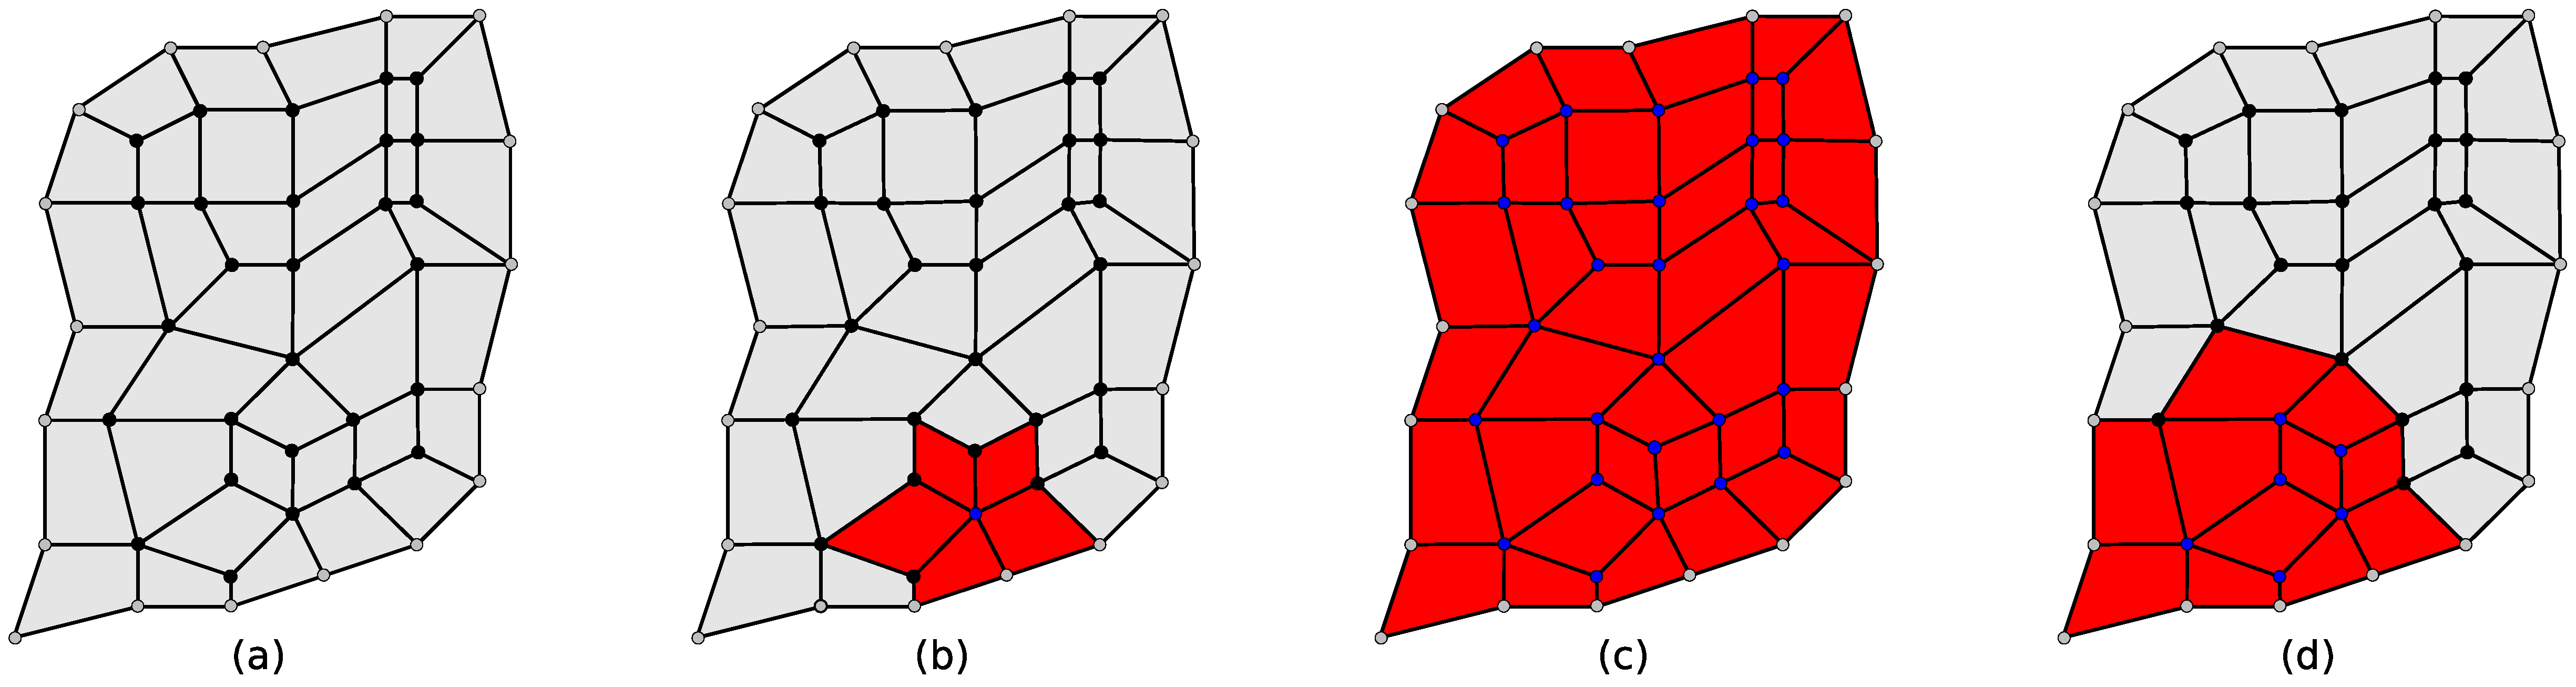
\includegraphics[width=5in]{patches-horiz}
\caption{Miscellaneous patch configurations.\label{fig:patch-types}}
\end{figure}

The global patch is a ``decomposition'' where the entire mesh is contained in a single patch.  This is used in the global optimization strategy discussed in Section \ref{sec:global}. Figure \ref{fig:patch-types}c illustrates the global patch.

The element-on-vertex decomposition subdivides the mesh into a single patch for each free vertex.  Each patch includes the layer of elements adjacent to the free vertex.  A element-on-vertex patch is illustrated in Figure \ref{fig:patch-types}b.  This decomposition is typically used for all optimization strategies discussed in this chapter except for global optimization.  Any other decomposition except global may be used for any of the optimization strategies.  All of the discussed strategies other than global do not make sense for a global patch.

Any patch decomposition can be used with Mesquite.  While no other decomposition strategy is provided with Mesquite, the any implementation of the {\texttt PatchSet} interface can be associated with any quality improver that supports it (any subclass of {\texttt PatchSetUser}, currently all except {\texttt LaplacianSmoother}).  An implementation of that interface is expected to provide three things:
\begin{enumerate}
\item An enumeration of all the patches in the decomposition of the mesh
\item For each patch, the set of vertices to optimize
\item For each patch, the set of elements for which the quality is to be optimized (typically all elements containing the vertices to be optimized.)
\end{enumerate}
A normal decomposition will be done such that each free vertex in the mesh is optimized in exactly one patch, but Mesquite does not enforce this.  Having a free vertex be optimized in no patch will result in that vertex effectively being fixed for the optimization.  A decomposition that optimized the same vertices in multiple patches is allowable, and should have no adverse side effects unless doing a Jacobi optimization (Section \ref{sec:jacobi}).

The listing below shows how a custom implementation of the {\texttt PatchSet} interface can be used with the {\texttt SteepestDescent} solver.

\begin{lstlisting}[frame=single]
MyMeshDecomposition my_patch_set;
SteepestDescent quality_improver( &objective_function );
\<quality_improver.use_patch_set(&my_patch_set);\>
\end{lstlisting}

In any of the examples later in this chapter that call {\texttt use\_element\_on\_vertex\_patch()}, that call may be substituted with a call to {\texttt use\_patch\_set} to use some decomposition other than single-vertex patches.


\section{PatchSetUser and PatchSet}

A \texttt{PatchSetUser} is an optimizer for which the application may specify how the mesh is decomposed into patches.  \texttt{PatchSetUser} provides two pre-defined patch schemes.  The \texttt{use\_global\_patch()} method will result in a single patch containing the entire mesh.  The \texttt{use\_element\_on\_vertex\_patch()} method will result in a patch for every free vertex in the mesh, containing only the free vertex and its adjacent elements.  An alternate scheme for subdividing the mesh into patches may be specified by providing a custom implementation of the \texttt{PatchSet} interface.

The \texttt{PatchSet} interface defines two methods: \texttt{get\_patch\_handles} and \texttt{get\_patch}.  The \texttt{get\_patch\_handles} method returns a list of handles (or identifiers), one for each potential patch in a mesh.  The \texttt{get\_patch} method returns the free vertices and elements in a patch, given one of the handles passed back from the \texttt{get\_patch\_handles} method.

The \texttt{GlobalPatch} class is the implementation of the \texttt{PatchSet} interface that provides a single patch for the entire mesh.  The \texttt{VertexPatches} class provides the Laplacian-like decomposition of the mesh into a patch for every free vertex.  The \texttt{ElementPatches} class is used internally in places other than the main optimization loop, such as initializing BCD data and in the \texttt{QualityAssessor} class.  It decomposes the mesh into single-element patches with no free vertices.


\section{Global \label{sec:global}}

For a global optimization an objective function that measures the quality of the mesh is minimized using a numerical solver.  The coordinates of all of the free vertices in the mesh are the free variables in the optimization.  This is the default mode of operation for most solver-based implementations of the {\texttt QualityImprover} interface.

A global optimization is simplest form of the generalized optimization loop.  In this mode the mesh is ``decomposed'' into a single patch containing the entire mesh.  The outer loops in Figure \ref{fig:genoptloop} are executed only once.  The entire optimization process happens in the inner loop.  For global optimization the outer termination criterion is the default of a single iteration.  The inner termination criterion should be used to terminate the optimization process.  Setting some other outer termination criterion is not prohibited, but will result in a much less efficient optimization process.  There is no logical difference between inner and outer termination criterion, but each iteration of the outer loop begins with a clean solver state which will result in less efficient operation of the solver.  Even steepest descent, the simplest solver, calculates a initial step size based on the previous iteration of the inner loop.  

The listing below shows how global optimization can be selected.

\begin{lstlisting}[frame=single]
// Create global optimizer instance
SteepestDescent improver( &objective_function );
\<improver.use_global_patch();\>

// Set only inner termination criterion for 
// global optimization
TerminationCriterion inner;
inner.add_absolute_vertex_movement( 1e-3 );
improver.set_inner_termination_criterion( &inner );

// Run optimization
InstructionQueue queue;
queue.set_master_quality_improver( &improver, err );
queue.run_instructions( &mesh, err );
\end{lstlisting}


\section{Nash Game vs. Block Coordinate Descent}

Quality improvers that have an explicit \texttt{ObjectiveFunction} may be used with the block coordinate descent algorithm rather than the default Nash game algorithm if the \texttt{ObjectiveFunction} implementation supports this mode of operation. In a Nash game optimization (the default), the objective function that is optimized by the inner loop is evaluated over only the patch being optimized.  In a block coordinate descent algorithm, the objective function to be optimized in the inner loop is evaluated over the entire mesh.  Only the influence of the current patch vertices on the global objective function is considered during the optimization of each patch.

\section{Nash Game \label{sec:nash} }


\begin{lstlisting}[frame=single]
// Create Nash optimizer instance
SteepestDescent improver( &objective_function );
\<improver.use_element_on_vertex_patch();\>

// Set inner and outer termination criterion for 
// non-global patch
TerminationCriterion inner, outer;
outer.add_absolute_vertex_movement( 1e-3 );
inner.add_iteration_limit( 2 );
improver.set_outer_termination_criterion( &outer );
improver.set_inner_termination_criterion( &inner );

// Run optimization
InstructionQueue queue;
queue.set_master_quality_improver( &improver, err );
queue.run_instructions( &mesh, err );
\end{lstlisting}


\section{Block Coordinate Descent \label{sec:bcd} }

\begin{lstlisting}[frame=single]
// Create BCD optimizer instance
SteepestDescent improver( &objective_function );
improver.use_element_on_vertex_patch();
\<improver.do_block_coordinate_descent_optimization();\>

// Set inner and outer termnation criterion for 
// non-global patch
TerminationCriterion inner, outer;
outer.add_relative_quality_improvement( 1e-2 );
inner.add_iteration_limit( 2 );
improver.set_outer_termination_criterion( &outer );
improver.set_inner_termination_criterion( &inner );

// Run optimization
InstructionQueue queue;
queue.set_master_quality_improver( &improver, err );
queue.run_instructions( &mesh, err );
\end{lstlisting}


\section{Culling \label{sec:culling}}


\begin{lstlisting}[frame=single]
// Create Nash optimizer with culling
SteepestDescent improver( &objective_function );
improver.use_element_on_vertex_patch();

// The culling criterion is effectively an outer 
// termination criterion because optimization will 
// always stop when all patches are culled.  We 
// must explicitly pass an empty outer termination 
// criterion to replace the default of one iteration.
// Additional outer termination criteria may also be 
// specifed.
TerminationCriterion inner, outer;
\<inner.cull_on_absolute_vertex_movement( 1e-3 );\>
inner.add_iteration_limit( 2 );
improver.set_outer_termination_criterion( &outer );
improver.set_inner_termination_criterion( &inner );

// Run optimization
InstructionQueue queue;
queue.set_master_quality_improver( &improver, err );
queue.run_instructions( &mesh, err );
\end{lstlisting}

\section{Jacobi \label{sec:jacobi}}

\begin{lstlisting}[frame=single]
// Create Jacobi optimizer instance
SteepestDescent improver( &objective_function );
improver.use_element_on_vertex_patch();
\<improver.do_jacobi_optimization();\>

// Set inner and outer termination criterion for 
// non-global patch
TerminationCriterion inner, outer;
outer.add_absolute_vertex_movement( 1e-3 );
inner.add_iteration_limit( 2 );
improver.set_outer_termination_criterion( &outer );
improver.set_inner_termination_criterion( &inner );

// Run optimization
InstructionQueue queue;
queue.set_master_quality_improver( &improver, err );
queue.run_instructions( &mesh, err );
\end{lstlisting}



% Constructing custom solvers - part 1
%\chapter{Constructing Custom Optimization Algorithms}

\section{Algoritm Components}




\section{Quality Metrics}

\section{Objective Functions}

\section{Solvers}

\section{Termination Criteria \label{sec:termination}}


% TMP
%\chapter{Quality Metrics and the Target Matrix Paradigm}

\section{Quality Metric Components}

\section{Target Metrics}

\section{Target Calculators}

\section{Metric Weights}

\section{Custom Target Calculators}



% more TMP stuff
%\chapter{Target Matrix Paradign Advanced Topics}

\section{Inital Mesh and Reference Meshes}

\section{Saving/Restoring Pre-Calculated Targets}

\section{Misc}

\subsection{Caching Targets}



% debugging solvers
\chapter{Analyzing Optimizer Behavior}

This chapter provides a brief overview of some of the tools provided in Mesquite for assisting with the analyze and visualization of the Mesquite optimization process.  The tools discussed in this section can be used to provide additional
output.  External tools such as Paraview, VisIt, or GNU Plot must be used to visualize the data.

\section{Debug Output}

Mesquite contains a mechanism to send status and debug messages to an output stream (e.g. {\texttt stdout} or {\texttt std::cout}).  Debug messages are grouped into logical categories identified by an integer number.  For example debug flag 1 refers to warnings.  Debug flag 2 is used for status information about the outer optimization loop, and debug flag 3 is used for status of the inner optimization loop. 

Debug flags can be controlled through a variety of means.  The {\texttt --enable-debug-output} configure option can be specified with a comma-separated list of integer values to specify which debug groups should be enabled by default.  An application may call the {\texttt MsqDebug::enable(unsigned)} and {\texttt MsqDebug::disable(unsigned)} functions to enable or disable debug message groups.  Debug message groups may also be controlled with the environmental variables {\texttt MESQUITE\_DEBUG} and {\texttt MESQUITE\_NO\_DEBUG}.  Each should have a comma-separated list of integer values as its argument.  The variables enable and disable, respectively, the corresponding debug message groups.

\section{Plotting Convergence Behavior \label{sec:optplot}}

The Mesquite {\texttt TerminationCriterion} class can produce a simple table of tab-separated values for the different Mesquite termination criterion.  This file can be used to plot the behavior of the optimization loop using GNU Plot, a spread sheet application, or any other suitable tool.  The code listing below illustrates how this feature is activated.

\begin{lstlisting}[frame=single]
// Create global optimizer instance
SteepestDescent improver( &objective_function );
improver.use_global_patch();

// Set only inner termination criterion for 
// global optimization
TerminationCriterion inner;
inner.add_absolute_vertex_movement( 1e-3 );
\<inner.write_iterations( "plot.gpt" );\>
improver.set_inner_termination_criterion( &inner );

// Run optimization
InstructionQueue queue;
queue.set_master_quality_improver( &improver, err );
queue.run_instructions( &mesh, err );
\end{lstlisting}

For usable results the feature must be activated on the appropriate {\texttt TerminationCriterion} instance.  For a global optimization it should be enabled for the {\em inner} termination criterion.  For other optimization strategies (see Chapter \ref{ch:optstrat}) it should be enabled for the {\em outer} termination criterion.  

The following is a sample output file:

\begin{lstlisting}[basicstyle=\small,language=sh]
#Iter	CPU	ObjFunc	GradL2	GradInf	Movement	Inverted
0	0	1.47419	0	0	0	0
1	0	1.147	0	0	0.657155	0
2	0	1.04779	0	0	0.402173	0
3	0	1.00572	0	0	0.357444	0
4	0	1.00006	0	0	0.150652	0
5	0	1	0	0	0.0153396	0
6	0	1	0	0	0.00015034	0
7	0	1	0	0	6.40008e-09	0
\end{lstlisting}

Notice that several of the columns contain only zeros.  The column containing the iteration number will always contain valid values.  Other values will only be included if they are calculated during the optimization loop.  The objective function value will be included for any global optimization that uses an explicit objective function (currently any optimizer other than {\texttt LaplacianSmoother}).  In the example source code above we are using the steepest descent solver with a global patch so the objective function value is also included.  The other values will only be present if they are calculated for the purpose of checking termination criteria.  In the example source code we specify a termination criterion based on vertex movement, so the column labeled ``movement'' contains the maximum distance any vertex was moved for the corresponding iteration.  

Figures \ref{fig:iterplot} shows the result of using the above data file with the following GNU Plot commands:
\begin{verbatim}
set xlabel 'iterations'
set ylabel 'objective function value'
set y2label 'maximum vertex movement'
set y2tics 0.1
plot 'plot.gpt' using 1:3 with linespoints \
     title 'objective function', \
     'plot.gpt' using 1:6 axes x1y2 with \
     linespoints title 'vertex movement'
\end{verbatim}

\begin{figure}[htb!]
\begin{center}
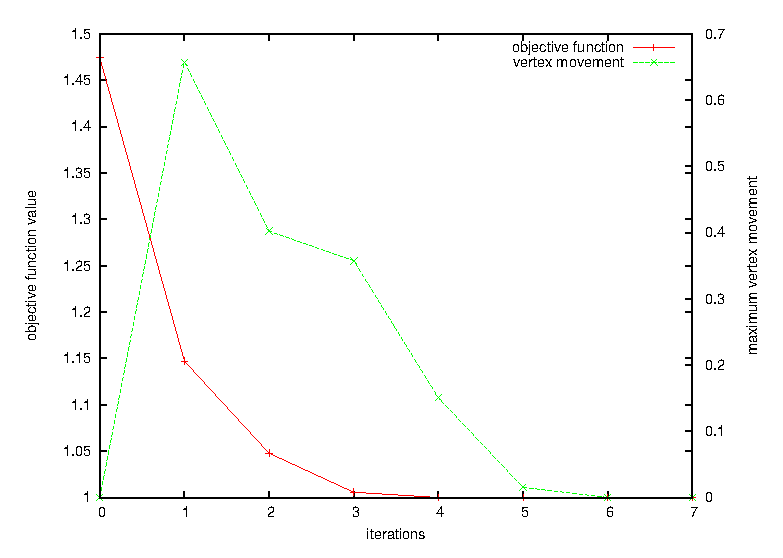
\includegraphics[width=5in]{iterplot}
\caption{\em Convergence Plot \label{fig:iterplot}}
\end{center}
\end{figure}

\section{Viewing Meshes}

VTK files read and written by the {\texttt MeshImpl} class are viewable in a plethora of visualization tools that use the VTK visualization library.  

The {\texttt Mesquite::MeshWriter} namespace contains functions to export mesh in a variety of formats for visualization including:
\begin{itemize}
\item GNU Plot
\item Visualization TookKit (VTK)
\item Encapsulated PostScript (EPS)
\item Scalable Vector Graphics (SVG)
\item StereoLithography (STL)
\end{itemize}
The GNU plot format writes line data that can be used to plot a wireframe of the mesh (the mesh edges).  Both 2D and 3D meshes can be exported in this format.  A mesh can be plotted as a 2D projection with the GNU plot command:
\begin{verbatim}
plot 'filename' with linespoints
\end{verbatim}
or as a rotatable 3D plot with the command:
\begin{verbatim}
splot 'filename' with linespoints
\end{verbatim}
Figure \ref{fig:meshgpt} is the result of plotting the mesh contained in {\texttt testSuite/higher\_order/homogeneousPart.vtk} with GNU plot.

\begin{figure}[htb!]
\begin{center}
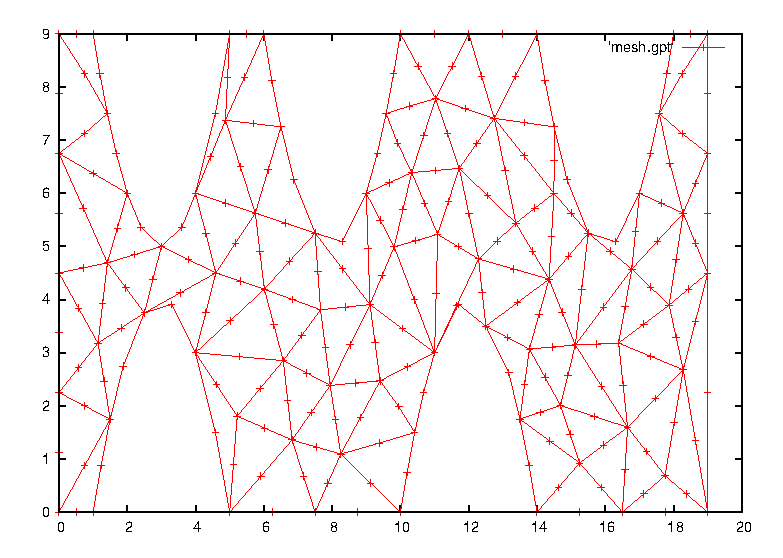
\includegraphics[width=4in]{mesh_gpt}
\caption{\em GNU Plot of 2D Quadratic Triangles \label{fig:meshgpt}}
\end{center}
\end{figure}

As mentioned in the previous section, the VTK file format can be used with a variety of visualization tools.  Figure \ref{fig:meshvtk} shows a simple plot of the same mesh in the Paraview visualization tool.

\begin{figure}[htb!]
\begin{center}
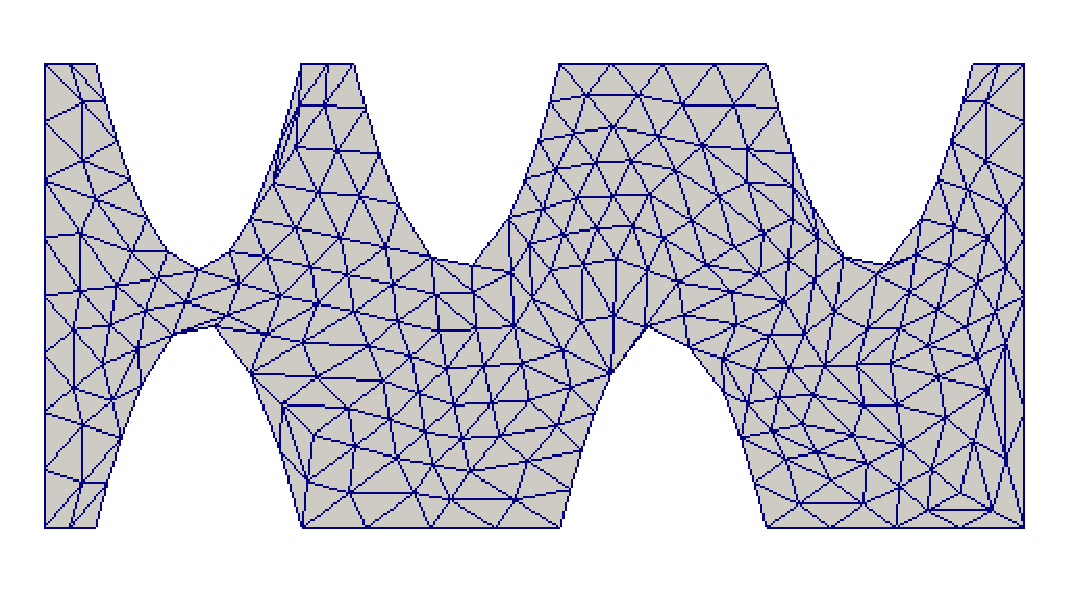
\includegraphics[width=4in]{mesh_vtk}
\caption{\em Paraview plot of 2D Quadratic Triangles \label{fig:meshvtk}}
\end{center}
\end{figure}

Figure \ref{fig:mesh} shows the output of the encapsulated PostScript writer for the mesh.  The EPS writer can write only 2D projections of the mesh.  The caller must specify a projection when calling {\texttt MeshWriter::write\_eps}.  The {\texttt testSuite/higher\_order/homogeneousPart.vtk} file contains quadratic triangle elements.  Compare the mesh edges on the mesh boundary in this plot with the output in Figures \ref{fig:meshgpt} and \ref{fig:meshvtk}.  The EPS writer in Mesquite exports the quadratic edges as curves corresponding to the classic quadratic edge shape function:
\begin{displaymath}
E(u) = \frac{1}{2}u(u-1)V_1 + (1-u^2)V_2 + \frac{1}{2}u(u+1)V_3
\end{displaymath}

\begin{figure}[htb!]
\begin{center}
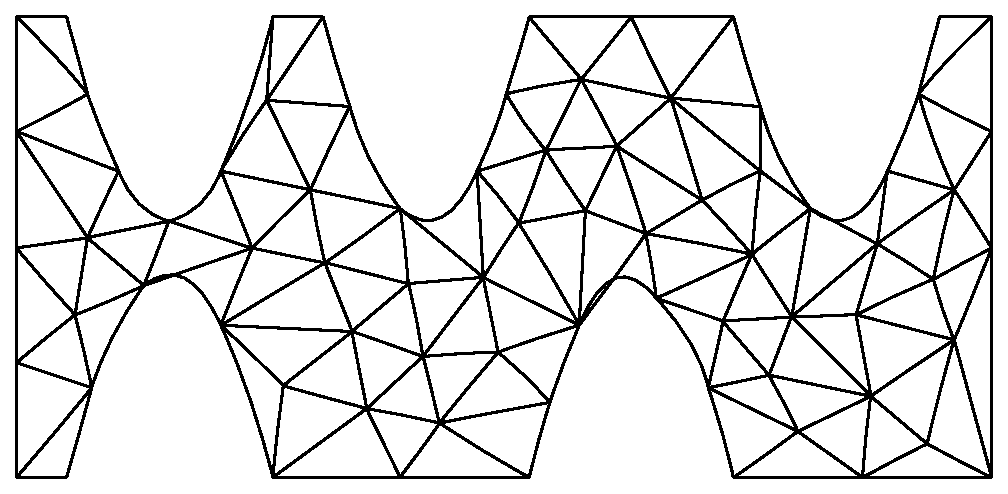
\includegraphics[width=4in]{mesh}
\caption{\em Encapsulated PostScript of 2D Quadratic Triangles \label{fig:mesh}}
\end{center}
\end{figure}

The STL file format can be used to write only linear triangles.  Higher-order triangular elements will be written as linear triangles.  An error will be returned if the mesh contains other element types.

\section{Exporting Mesh Quality}

The {\texttt QualityAssessor} class has the ability to store mesh quality values and other characteristics as tag data on mesh elements.  This data can be accessed directly by applications or written to a VTK file using the {\texttt MeshImpl} class or the applications native mesh writer (if it is capable of writing tag data.)  The example code below was used to create the VTK file from which the Paraview plot in Figure \ref{fig:meshqual} was generated.

\begin{figure}[htb!]
\begin{center}
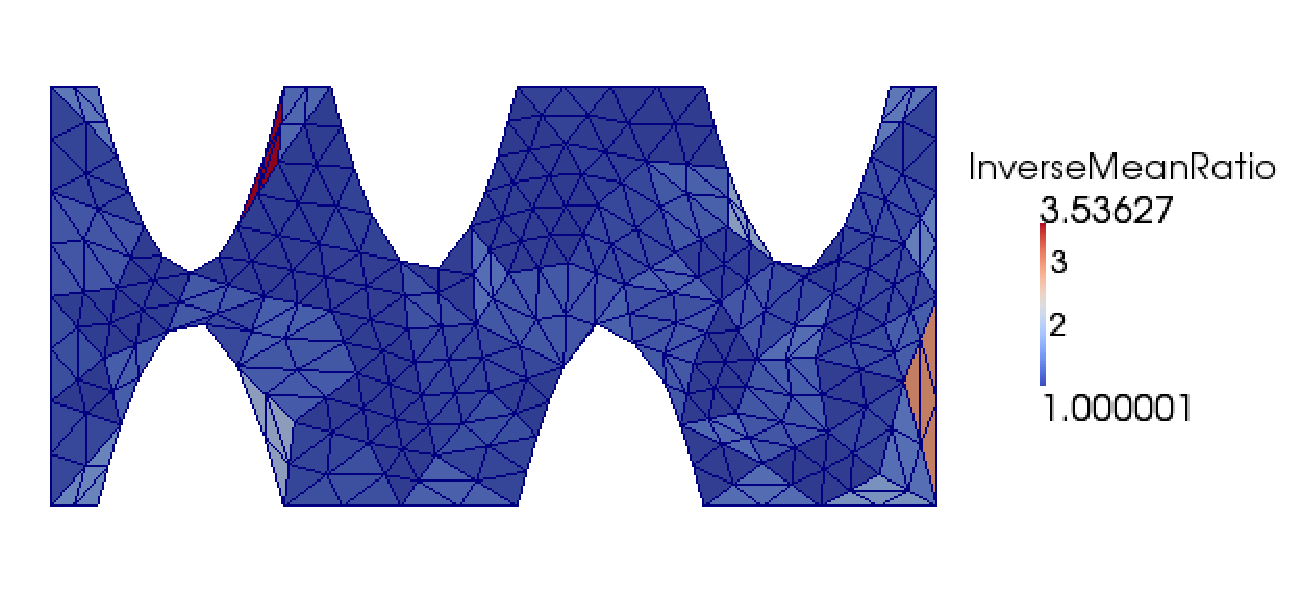
\includegraphics[width=5in]{meshqual}
\caption{\em Paraview Plot Coloring Elements by Quality Metric Value \label{fig:meshqual}}
\end{center}
\end{figure}

\begin{lstlisting}[frame=single]
MsqError err;
MeshImpl mesh;
mesh.read_vtk( "homogeneousPart.vtk", err );

IdealWeightInverseMeanRatio metric;
QualityAssessor qa;
qa.add_quality_assessment(&metric,0,0,0,\<"InverseMeanRatio"\>);

PlanarDomain plane(PlanarDomain::XY);
InstructionQueue queue;
queue.add_quality_assessor( &qa, err );
queue.run_instructions( &mesh, &plane, err );

mesh.write_vtk( "meshqual.vtk", err );
\end{lstlisting}

\begin{figure}[htb!]
\begin{center}
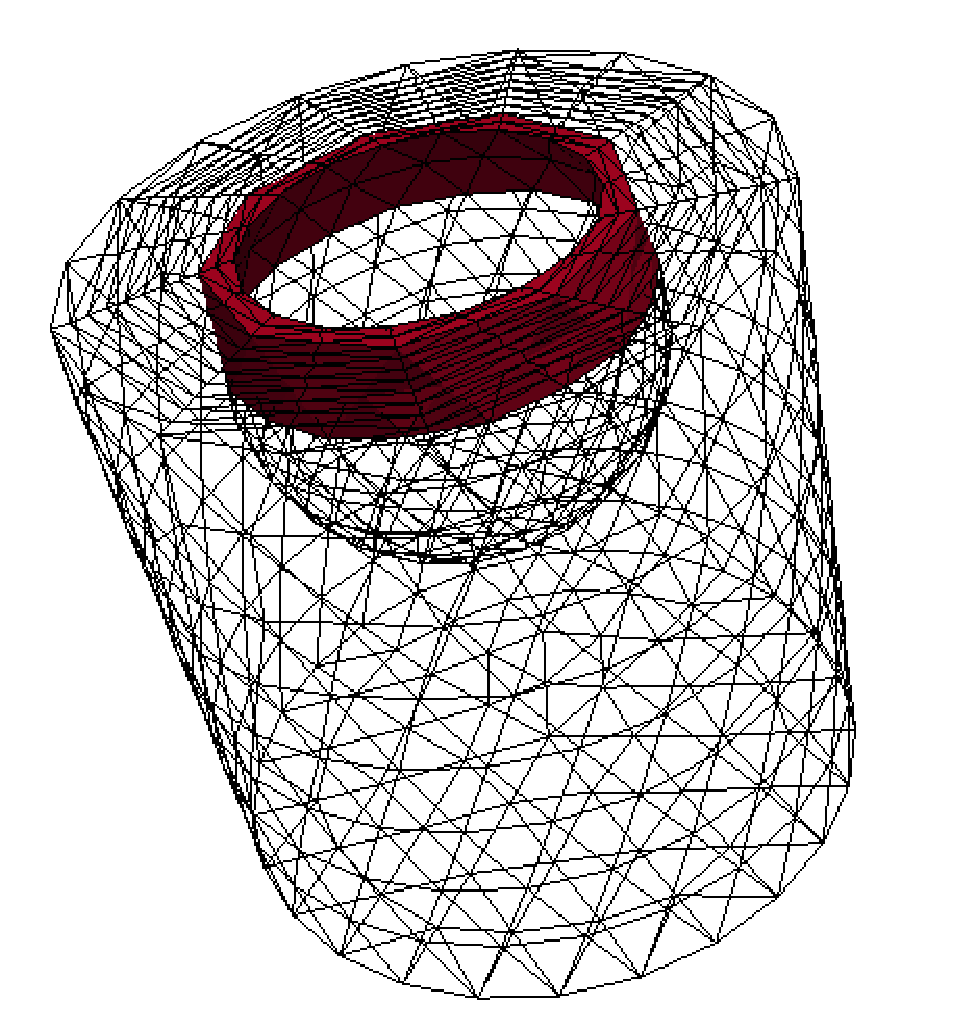
\includegraphics[width=3in]{meshqual3d}
\caption{\em Paraview Plot Showing Inverted Elements \label{fig:meshqual3d}}
\end{center}
\end{figure}

Figure \ref{fig:meshqual3d} is a Paraview plot showing the inverted elements in a quadratic tetrahedral mesh.  The mesh is plotted twice: once as a simple wireframe of the mesh boundary and a second time as solid mesh with a threshold filter on the inverted flag exported by Mesquite.  The listing below shows how the {\texttt QualityAssessor} class can be instructed to flag inverted elements:

\begin{lstlisting}[frame=single]
MsqError err;
MeshImpl mesh;
mesh.read_vtk( "sphereCylinder_1194_inv.vtk", err );

QualityAssessor qa;
\<qa.tag_inverted_elements("Inverted");\>

InstructionQueue queue;
queue.add_quality_assessor( &qa, err );
queue.run_instructions( &mesh, &plane, err );

mesh.write_vtk( "meshqual.vtk", err );
\end{lstlisting}


\section{Mesh Optimization Visualization}

The Mesquite {\texttt TerminationCriterion} class can write the complete mesh after each iteration as either VTK or GNU Plot data suitable for viewing as an animation.  Similar to requesting plot data as described in Section {\ref sec:optplot}, it is important to request this feature from the appropriate termination criterion instance.  If doing a global optimization, the feature should be activated for the {\em inner} termination criterion.  Otherwise the feature should almost always be activated for the {\em outer} termination criterion.  

The command to request an animation of the mesh optimization in the VTK format is:
\begin{lstlisting}
tc.write_mesh_steps( "anim", TerminationCriterion::VTK );
\end{lstlisting}
This will produce a sequence of files named ``anim.1.vtk'', ``anim.2.vtk'', etc.  The files can be opened in visualization tools such as Paraview as a single set and played back as an animation.  If the optimization calculates the gradient of the objective function, that data will also be included in the file as vector data on each mesh vertex.  The components of the vector on each vertex are the partial derivatives of the objective function with respect to each coordinate value of the vertex.  A Paraview ``glyph'' filter can be used to display these vector values during the animation.


The command to request an animation of the mesh optimization in a format suitable for animating in GNU plot is:
\begin{lstlisting}
tc.write_mesh_steps( "anim", TerminationCriterion::GNUPLOT );
\end{lstlisting}
This will produce a sequence of files named ``anim.1'', ``anim.2'', etc.  It will also export a file named ``anim'' that contains the necessary GNU Plot commands to display the animation.





% Parallel Mesquite
\chapter{Using Mesquite in Parallel}
\label{sec:parallel}

\section{Introduction}

Large meshes are often partitioned across many parallel processors either because they are too large to fit into the memory of a single machine or in order to speed up the computation. Even if it would be possible to assemble all partitions on a single processor, smooth the mesh, and repartition the result, such an approach would be very I/O inefficient. Moreover, for larger meshes such an approach would quickly run out of memory and fail. Therefore Mesquite supports smoothing meshes in parallel.

Mesquite currently does only synchronous Nash-game or local optimizations in parallel \cite{Fr95}.  It does not yet provide parallel solvers and therefore cannot do either block coordinate descent or truly global optimizations in parallel (minimization of an explicit, global objective function.)  

For algorithms such as Laplacian smoothing that are local optimizations, optimization in parallel is essentially the same as in serial.  For other optimizations that do a global minimization of an explicitly defined objective function in serial (for example \texttt{ShapeImprover}), the parallel optimization will be a Nash-game type optimization where the interior vertices (those not on the partition boundaries) will be optimized as a group.  Each vertex on the partition boundary will then be optimized individually.  While a global optimization in serial will typically have only one outer iteration, it is generally desirable to do multiple outer iterations in parallel so the Nash-game type optimization can reach convergence.  Mesquite wrappers (see Chapter \ref{sec:wrappers}) that implement global optimizations in serial default to 10 outer iterations in parallel.


\section{Distributed Mesh}

The input mesh for use in parallel quality improvement must be partitioned based on vertices.  That is, each vertex in the mesh must be assigned a single processor as its owner.  For optimal performance, vertices should be evenly distributed amongst available processors and the vertices assigned to the same processor should compose a contiguously connected patch of mesh.  

Each processor must also have access to all elements for which the position of its vertices influence the quality.  For almost all algorithms in Mesquite, this is the set of all elements that contain one of the vertices.  Further, each processor must also be able to access any additional vertices owned by other processors that are necessary to define those elements.  The instances of such vertices on processors that do not own them are typically referred to as ``ghosted'' vertices.  Elements for which copies exist on multiple processors may sometimes also be referred to as ``ghosted'' or ``ghost'' elements.

\begin{figure*}[htbp]
\begin{center}
    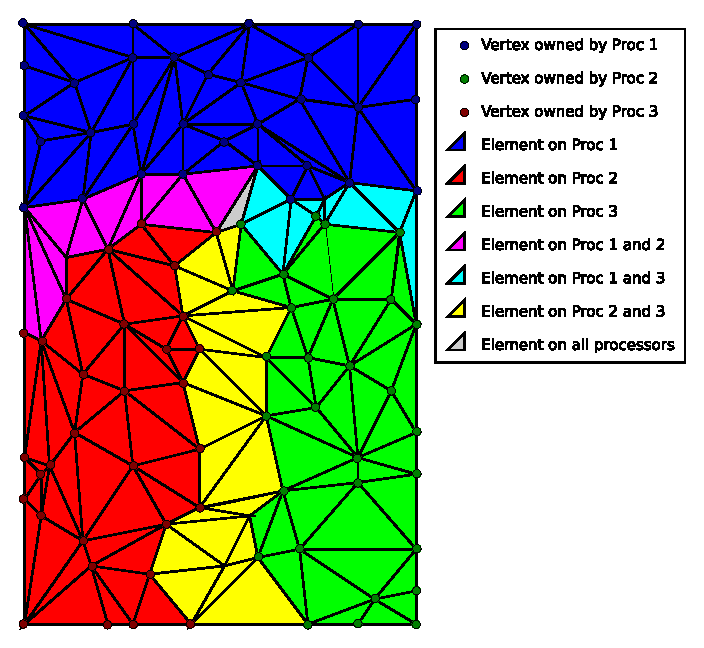
\includegraphics{parallel_mesh.eps}
    \caption{Sharing or ghosting of elements and vertices in a partitioned mesh.}
    \label{fig:parallel_mesh}
\end{center}
\end{figure*}

Figure \ref{fig:parallel_mesh} shows a mesh partitioned amongst three processors.  The vertices owned by the three different processors are shown in three different colors: blue, red, and green.  Elements are colored according to the processors for which copies of that element must be available.  A copy of an element must be available on each processor owning at least one of the vertices of the element.  Elements colored blue, red, or green need be visible only on the processor owning vertices of the corresponding color. The single grey element must have copies defined on all three processors because each of its vertices is owned by a different processor.  The remaining elements must be defined on at least two processors.  

For a copy of an element to be available on a processor, all of its vertices must also be available on that processor.  So for all elements for which copies exist on more than one processor, the vertices contained in those elements must also exist as ghost vertices on at least one processor.  That is, copies of such vertices must exist on processors other than those that are responsible for optimizing the location of that vertex.  For example, copies of the yellow elements in Figure \ref{fig:parallel_mesh} exist on both the blue and the green processors.  All blue vertices in at least one yellow element must exist as ghost vertices on the green processor and all green vertices in at least one yellow element exist as ghost copies on the blue processor.  A copy of the grey element must exist on every processor.  Therefore each vertex in that element exist as ghost copies on both of the other two processors that do not own it.  


\section{Input Data}

Assuming the mesh exists in partitioned form the user has to provide Mesquite with three things:
\begin{itemize}
\item a processor ID of type \texttt{int} for every vertex that determines which processor owns a vertex and is in charge for smoothing this vertex,
\item a global ID of type \texttt{size\_t} for every vertex that (at least in combination with the processor ID) is globally unique,
\item all necessary ghost elements and ghost nodes along the partition boundary must be provided.
\end{itemize}

The following copies of elements and vertices must exist: Elements must exist on all processors that own one or more of the vertices they reference. Vertices must exist on all processors that have some element referencing them.

The \texttt{Mesquite::ParallelMesh} class (\texttt{ParallelMeshInterface.hpp}) inherits \texttt{Mesquite::Mesh} and defines the interface Mesquite uses to interact with parallel mesh data. It contains the following additional pure virtual (or abstract) functions:
\begin{itemize}
\item get processor ids for given vertices,
\item get global ids for given vertices,
\item set and get a pointer to a \texttt{Mesquite::ParallelHelper} object.
\end{itemize}

To allow Mesquite direct access to the way you store the parallel mesh data you must inherit \texttt{Mesquite::ParallelMesh} and also implement your own get processor ID and get global ID functionality. The \texttt{Mesquite::ParallelHelper} class takes care of all the underlying communication using MPI. You will always use the \texttt{Mesquite::ParallelHelperImpl} implementation that we provide.

Alternatively you can turn any existing mesh of type \texttt{Mesquite::Mesh} into a parallel mesh of type\vspace{-5pt} \begin{center}
\texttt{Mesquite::ParallelMesh} by using the \texttt{Mesquite::ParallelMeshImpl} 
\end{center} \vspace{-5 pt}implementation we provide. On creation it needs a pointer to an object of type \texttt{Mesquite::Mesh} and the names of two tags. It is expected that every vertex is properly tagged with the processor ID tag being of type INT and the global ID tag being of type HANDLE.


\subsection{ParallelMesh Implementation Requirements}
%%(this text needs to be added where GLOBAL_ID etc is discussed)

In addition to global and processor ID's, a tag named \texttt{LOCAL\_ID}, with type \texttt{INT}, must be provided in
your ParallelMesh implementation.  In summary, here are the tags and
their types required by Parallel Mesquite:

\begin{tabular}{ | l | l | l | }
  \hline                        
  Concept name & Typical/required code string &  Mesquite type \\
\hline
 vertex processor owner id & \texttt{PROCESSOR\_ID} (typical, implementation-dependent) & INT \\
 vertex global unique id & \texttt{GLOBAL\_ID} (typical,  implementation-dependent) & HANDLE \\
 vertex local id (internal use) & \texttt{LOCAL\_ID} (required) & INT \\
  \hline  
\end{tabular}

If you obtained Mesquite from the Trilinos site, you can see a sample
imlementation of ParallelMesh in the stk\_percept package, at

\texttt{Trilinos/packages/stk/stk\_percept/stk\_percept/mesh/mod/mesquite-interface/PerceptMesquiteMesh.*pp}

\section{ITAPS iMeshP Interface}

The MsqIMeshP class is an alternate implementation of the \texttt{ParallelMesh} interface that can be used to provide Mesquite with callbacks to access mesh and related parallel properties.  The ITAPS Working Group has defined a standard API for exchange of parallel mesh data between applications. The \texttt{Mesquite::MsqIMeshP} class declared in \texttt{MsqIMeshP.hpp} is an ``adaptor'':  it presents the iMeshP interface as the \texttt{Mesquite::ParallelMesh} interface.  

This class will use the iMeshP API to query processor identifiers and global identifiers for mesh vertices.  However, the MPI-based communication routines implemented in \texttt{ParallelHelperImpl} are used rather to communicate updated vertex locations between processors, rather than the mechanism provided by the iMeshP implementation.

\section{Examples}

This section contains two different examples of simple stand-alone applications that demonstrate the use of the \texttt{LaplaceWrapper} smoother in parallel.  Both examples, in being stand-alone programs, load the mesh from one or more files.  When integrating Mesquite into an existing application where it is desired that Mesquite access application mesh data in memory, the initial setup will be different.  It will typically involve either providing some application-specific implementation of the \texttt{Mesh} and possibly \texttt{ParallelMesh} interfaces or instances of an appliction-specific \texttt{iMeshP} and \texttt{iMesh} implementation.

\subsection{Example: Parallel Laplacian Smooth}
\label{sec:parallel-example-1}

This example uses the \texttt{LaplaceWrapper} wrapper in parallel using the built-in \texttt{Mesh}, \texttt{ParallelMesh}, and \texttt{ParallelHelperImpl} implementations.  For this example to work, the mesh must be partitioned such that the mesh for each processor is saved in a separate file named \texttt{part-\%d.vtk}, with the \texttt{\%d} replaced with the processor rank.  Each VTK file must contain vertex attributes named \texttt{GID} and \texttt{PID} containing the global ID and owning processor rank for each vertex.  Further, as this example provides no geometric domain definition, the vertices on the boundary of the mesh must be designated as ``fixed'' for the problem setup to be valid.


\begin{verbatim}
/* Mesquite includes */
#include <Mesquite.hpp>
#include <MeshImpl.hpp>
#include <ParallelMeshImpl.hpp>
#include <ParallelHelper.hpp>
#include <MsqError.hpp>
#include <LaplaceWrapper.hpp>

/* other includes */
#include <mpi.h>
#include <iostream>
using namespace std;
  
int main( int argc, char* argv[] )
{
  /* init MPI */
  int rank, nprocs;
  if (MPI_SUCCESS != MPI_Init(&argc, &argv)) {
    cerr << "MPI_Init failed." << endl;
    return 2;
  }
  MPI_Comm_rank(MPI_COMM_WORLD, &rank);
  MPI_Comm_size(MPI_COMM_WORLD, &nprocs);

  /* create processor-specific file names */
  ostringstream in_name, out_name;
  in_name << "part-" << rank << ".vtk";
  out_name << "part-" << rank << "-smoothed.vtk";

  /* load different mesh files on each processor */
  Mesquite::MsqError err;
  Mesquite::MeshImpl mesh;
  mesh.read_vtk(in_name.str().c_str(), err);
  if (err) {cerr << err << endl; return 1;}

  /* create parallel mesh instance, specifying tags 
   * containing parallel data */
  Mesquite::ParallelMeshImpl parallel_mesh(&mesh, "GID", "PID");
  Mesquite::ParallelHelperImpl helper;
  helper.set_communicator(MPI_COMM_WORLD);
  helper.set_parallel_mesh(&parallel_mesh);
  parallel_mesh.set_parallel_helper(&helper);

  /* do Laplacian smooth */
  LaplaceWrapper optimizer;
  optimizer.run_instructions(&parallel_mesh, err);
  if (err) {cerr << err << endl; return 1; }

  /* write mesh */
  mesh.write_vtk(out_name.str().c_str(),err);
  if (err) {cerr << err << endl; return 1;}

  MPI_Finalize();
  return 0;
}
\end{verbatim}

\subsubsection{Implementation of Example \ref{sec:parallel-example-1} }

In your Mesquite distribution, there is an implementation of the
example code for Lapalace smoothing in parallel, in the file
\texttt{mesquite/testSuite/parallel\_smooth\_laplace/par\_hex\_smooth\_laplace.cpp}.
This code reads in a serial or parallel-split set of VTK files and
smooths the mesh, then compares the result to a "gold" copy, which is
useful for regression testing (see \ref{sec:RegressionTesting}).

\subsubsection{Parallel Regression Tests}

In addition to the Laplace example, see \\
\texttt{mesquite/testSuite/parallel\_untangle\_shape/par\_hex\_untangle\_shape.cpp} \\
for example use of parallel mesh untangling and shape improvement, and
the associated files:\\
\texttt{meshFiles/{2D,3D}/VTK/par\_*}

For example, an initial, tangled quadrilateral mesh is shown in
\ref{fig:par_quad_orig} 
while the result of untangling and smoothing is shown in
\ref{fig:par_quad_smoothed}.  A similar example with hexahedra is
shown in figures 
\ref{fig:par_hex_orig}  and \ref{fig:par_hex_smoothed}.

\begin{figure*}[htpb]
\begin{center}
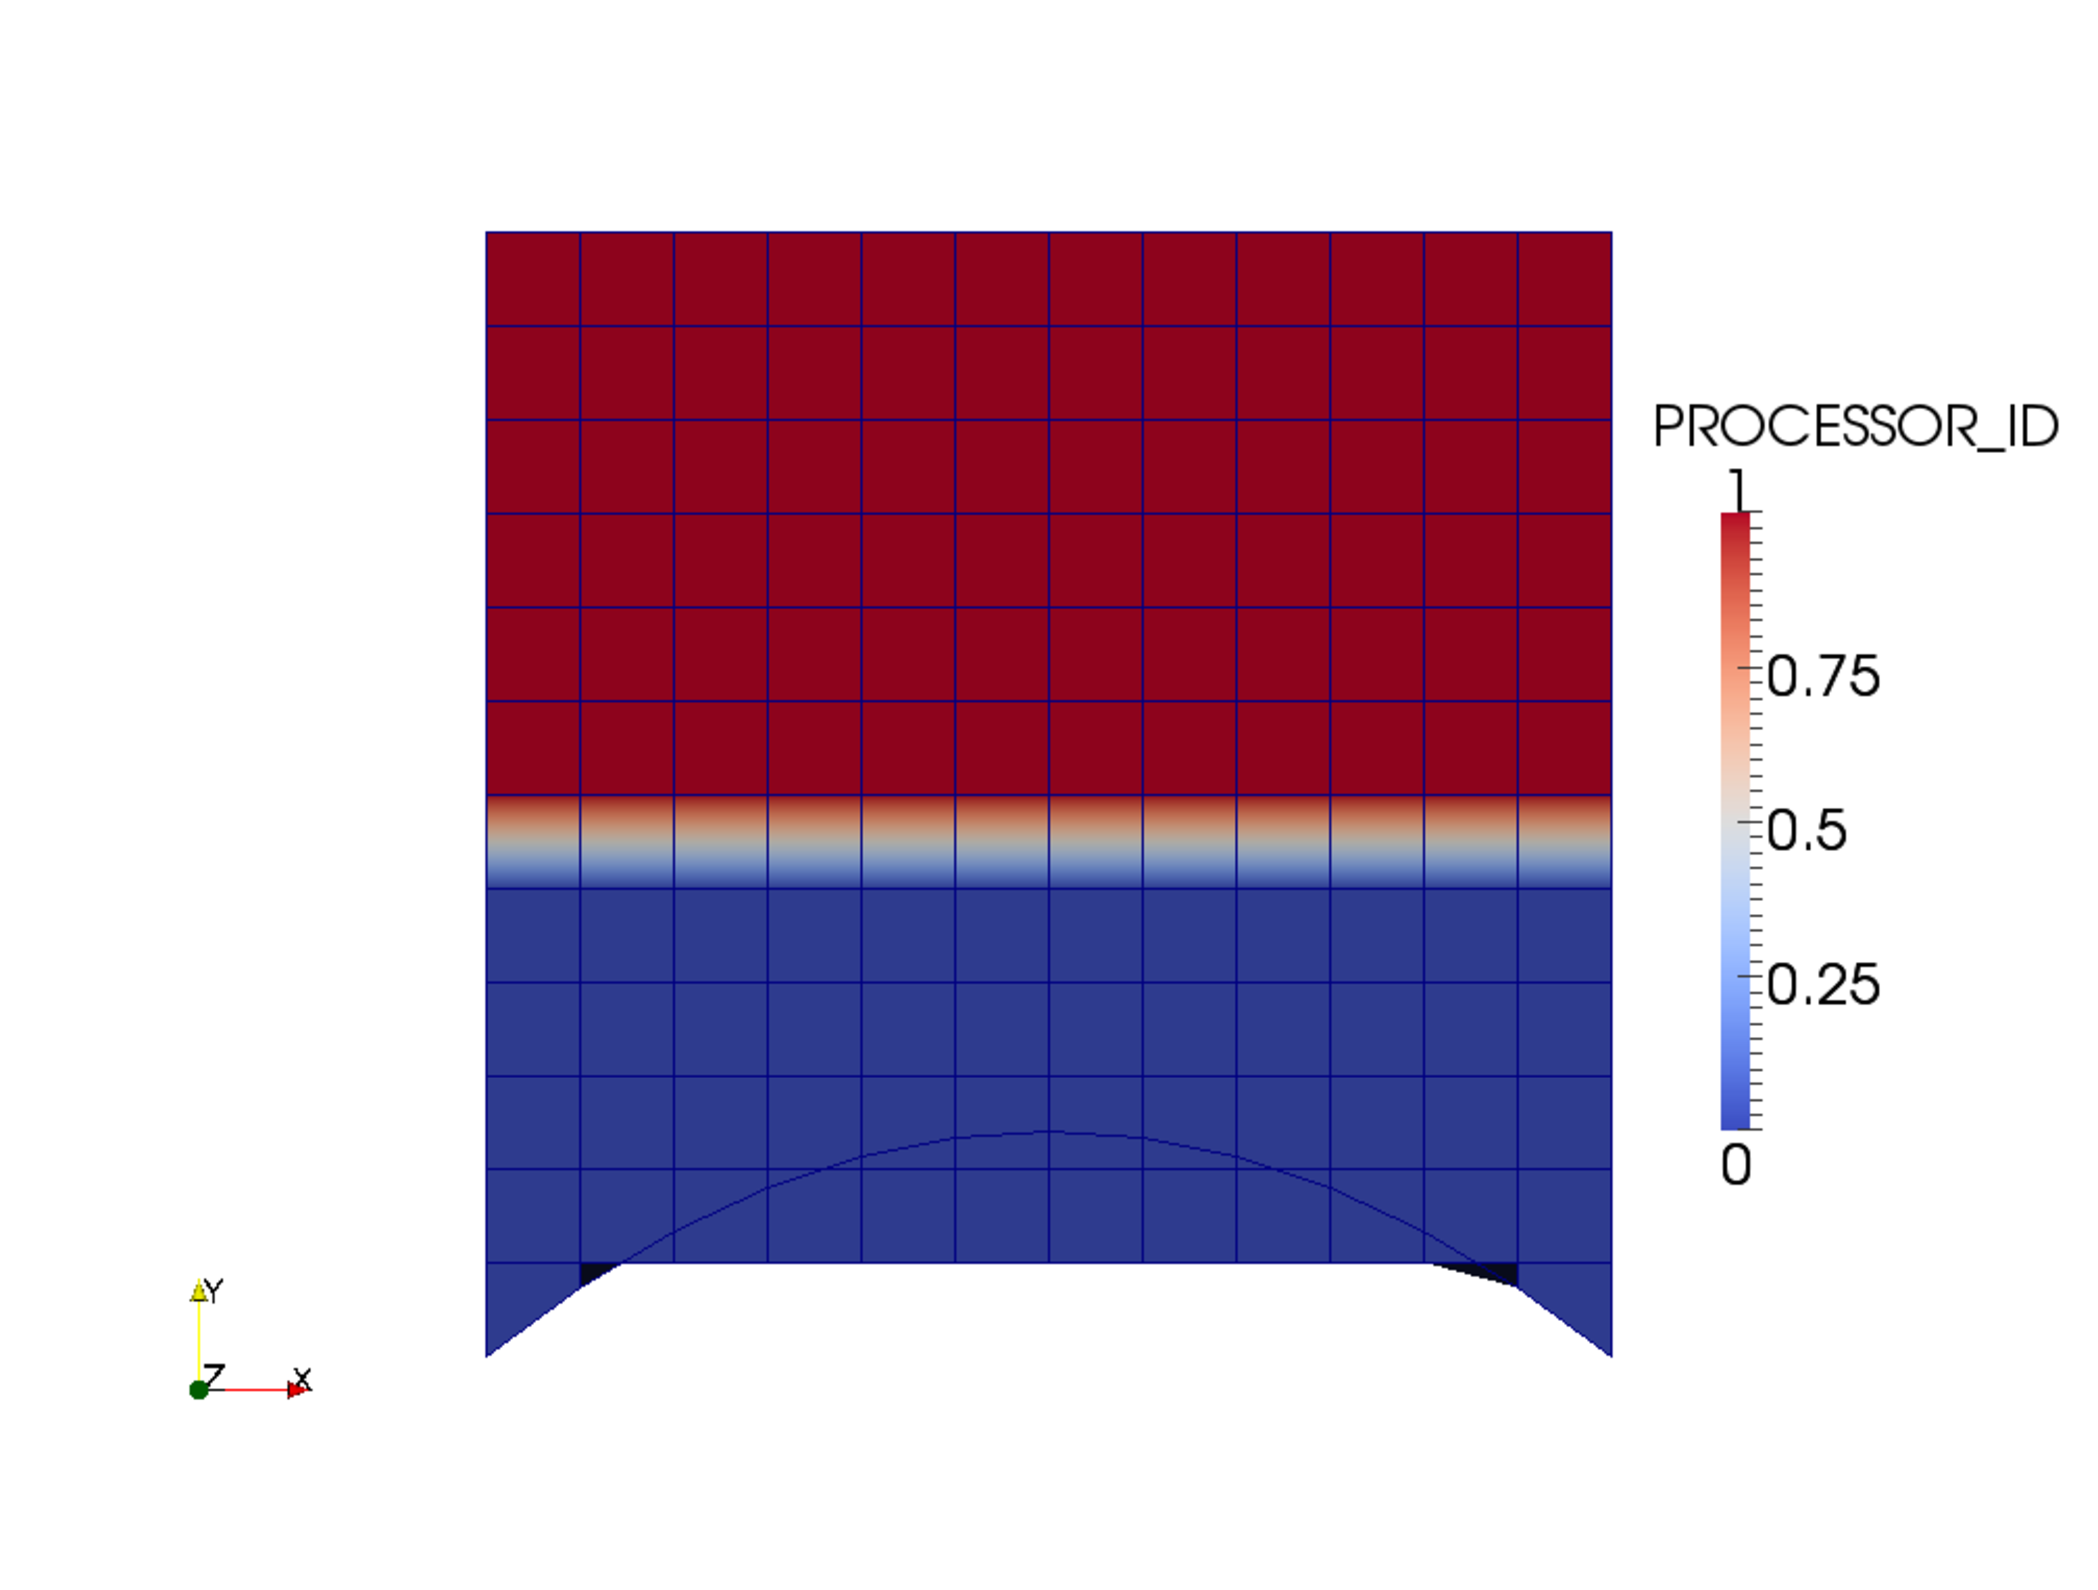
\includegraphics[width=4in]{par-quad-orig.eps}
\caption{Initial, tangled quadrilateral mesh.}
\label{fig:par_quad_orig}
\end{center}
\end{figure*}

\begin{figure*}[htpb]
\begin{center}
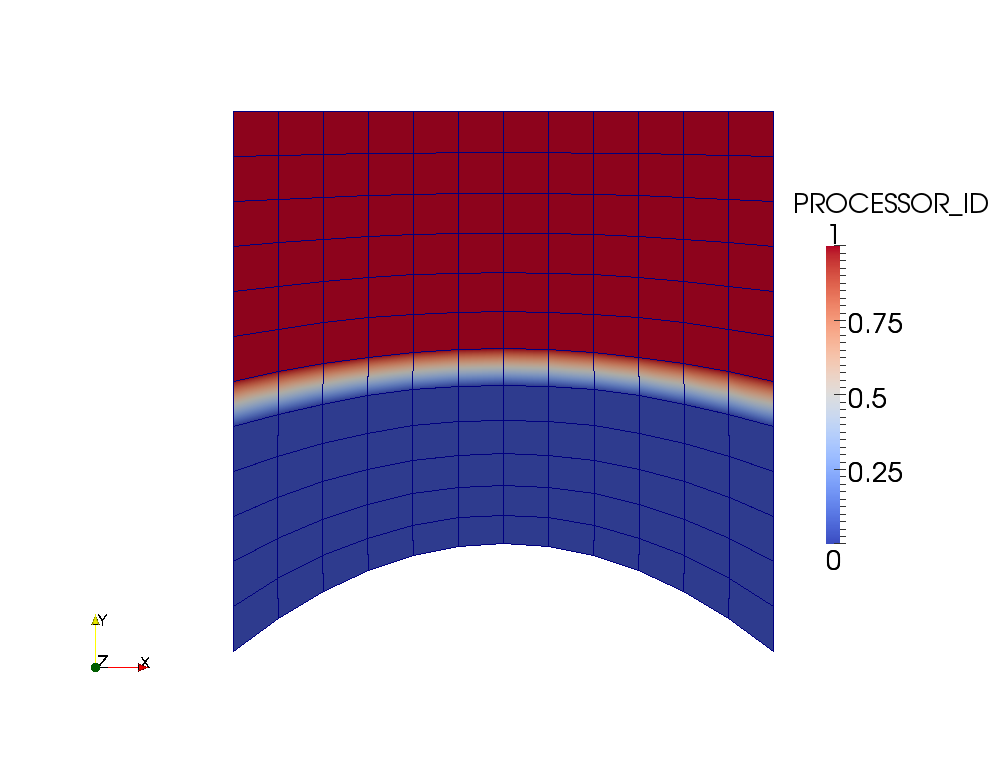
\includegraphics[width=4in]{par-quad-smoothed.eps}
\caption{Untangled and smoothed quadrilateral mesh.}
\label{fig:par_quad_smoothed}
\end{center}
\end{figure*}

\begin{figure*}[htpb]
\begin{center}
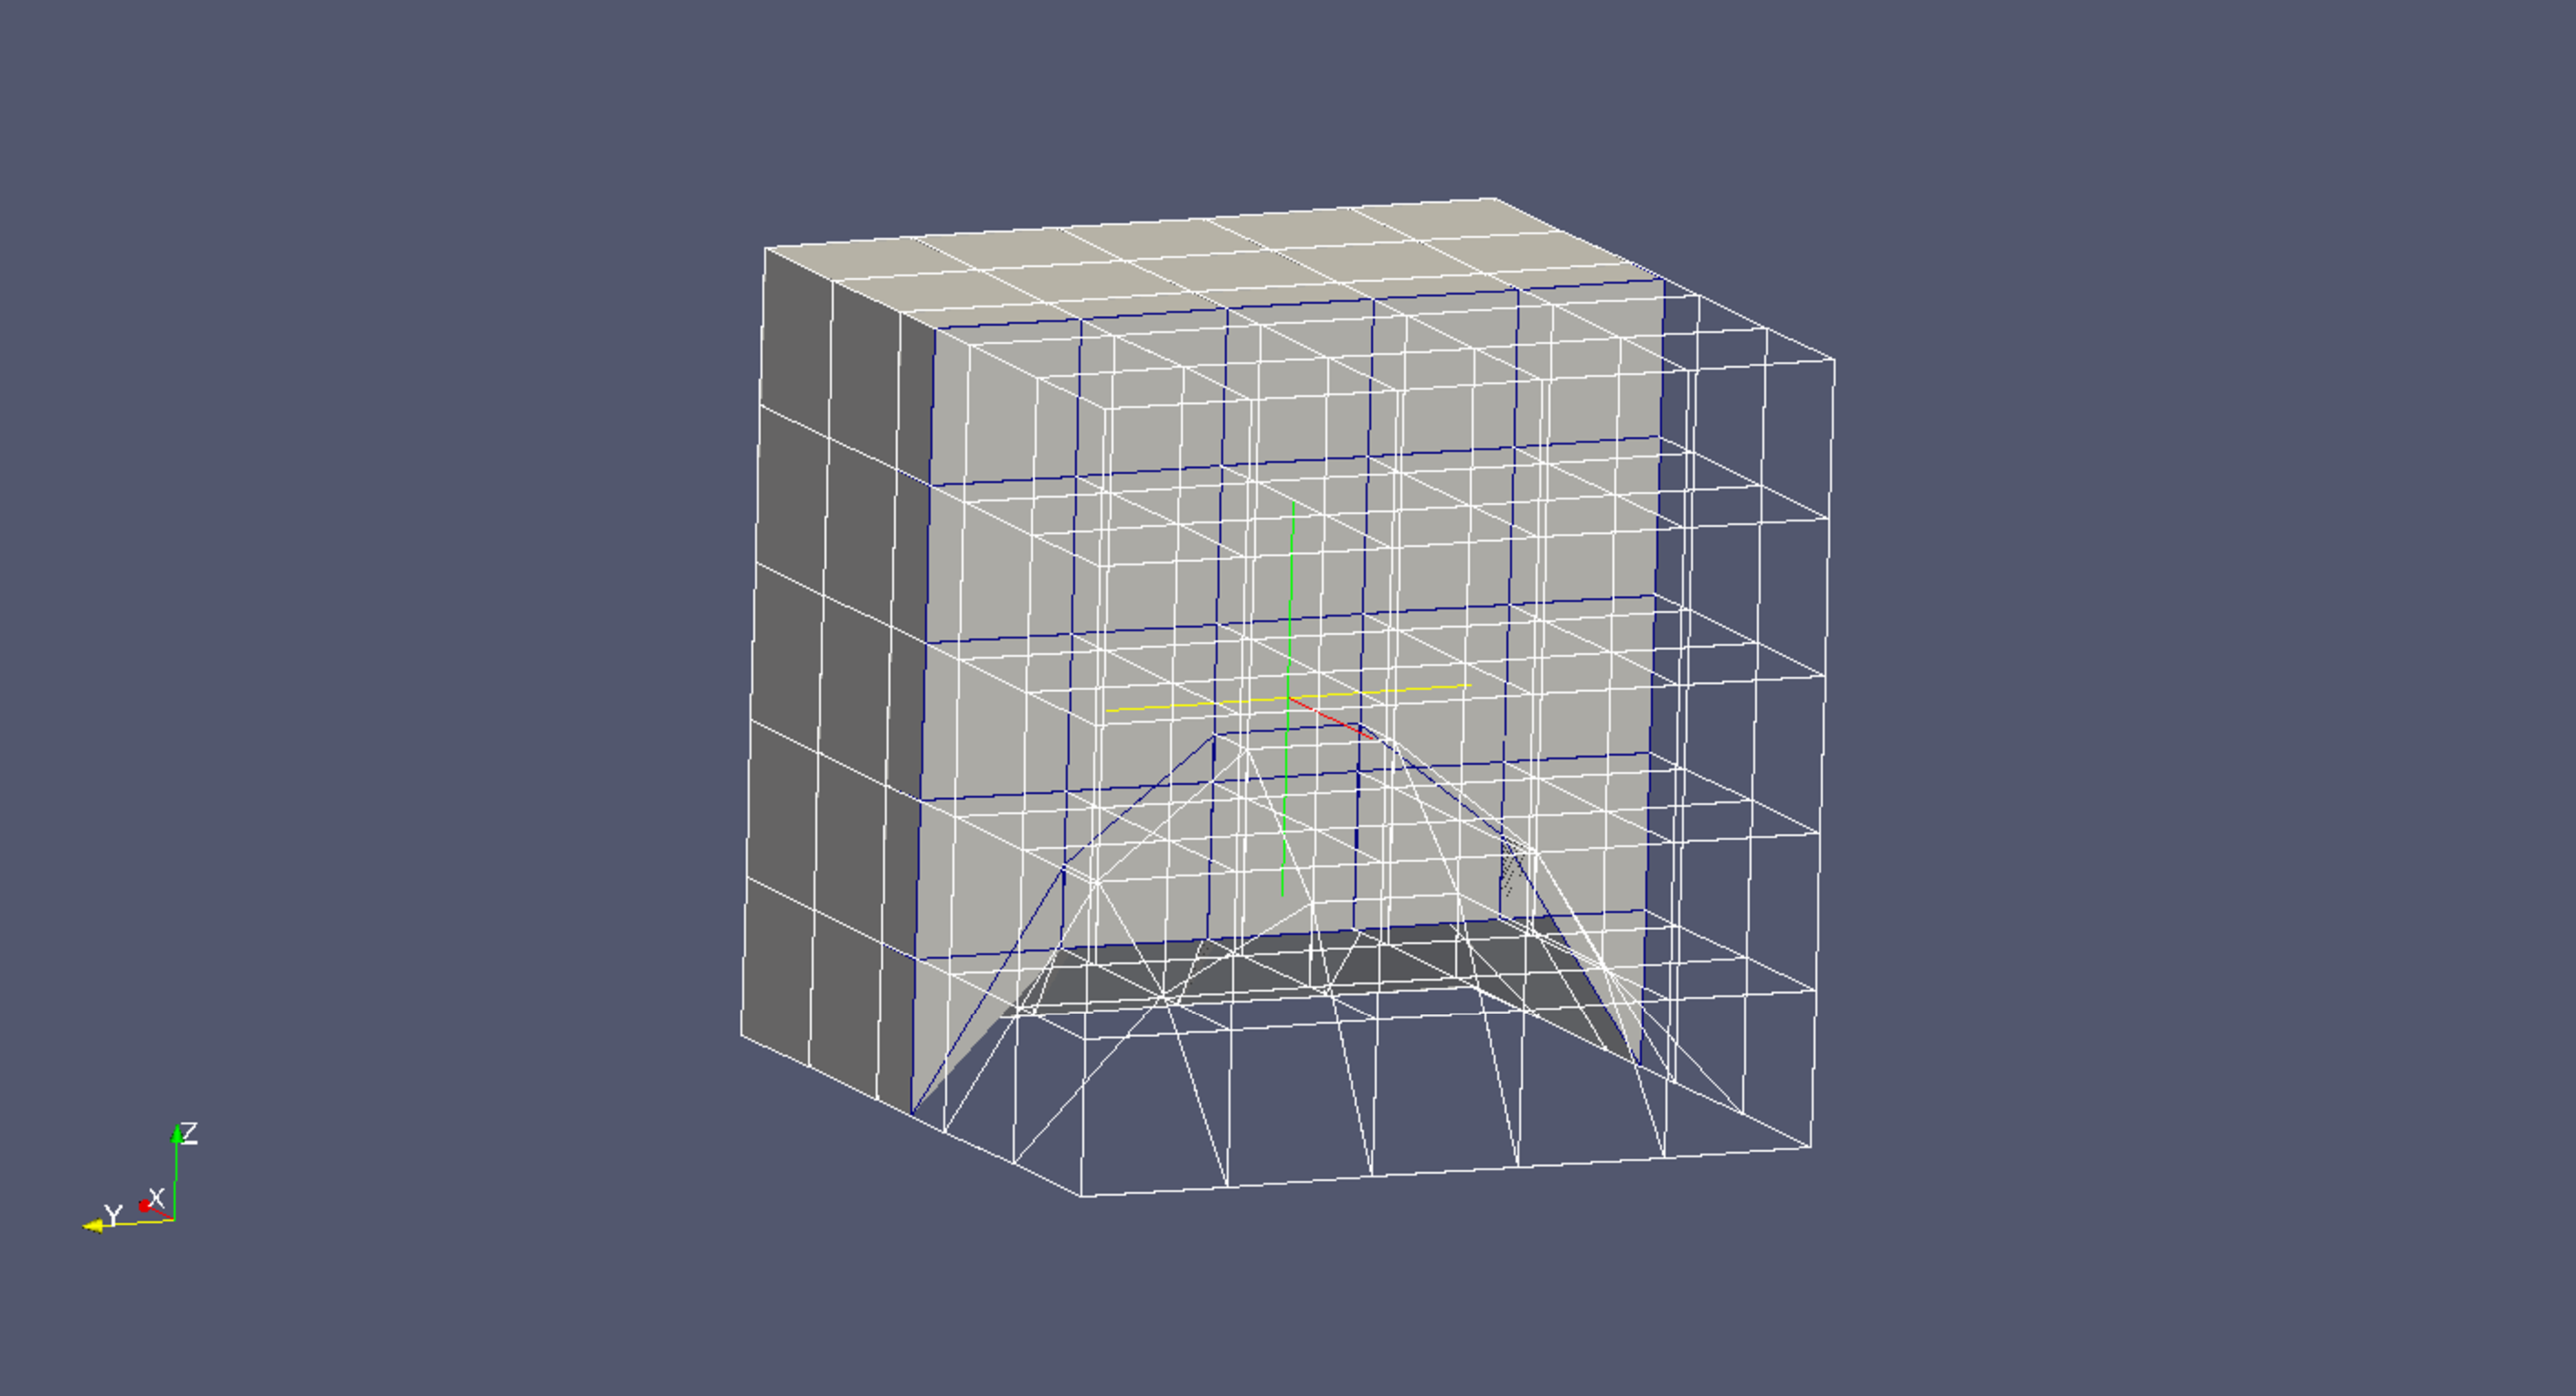
\includegraphics[width=4in]{par-hex-orig.eps}
\caption{Initial, tangled hexahedra mesh.}
\label{fig:par_hex_orig}
\end{center}
\end{figure*}

\begin{figure*}[htpb]
\begin{center}
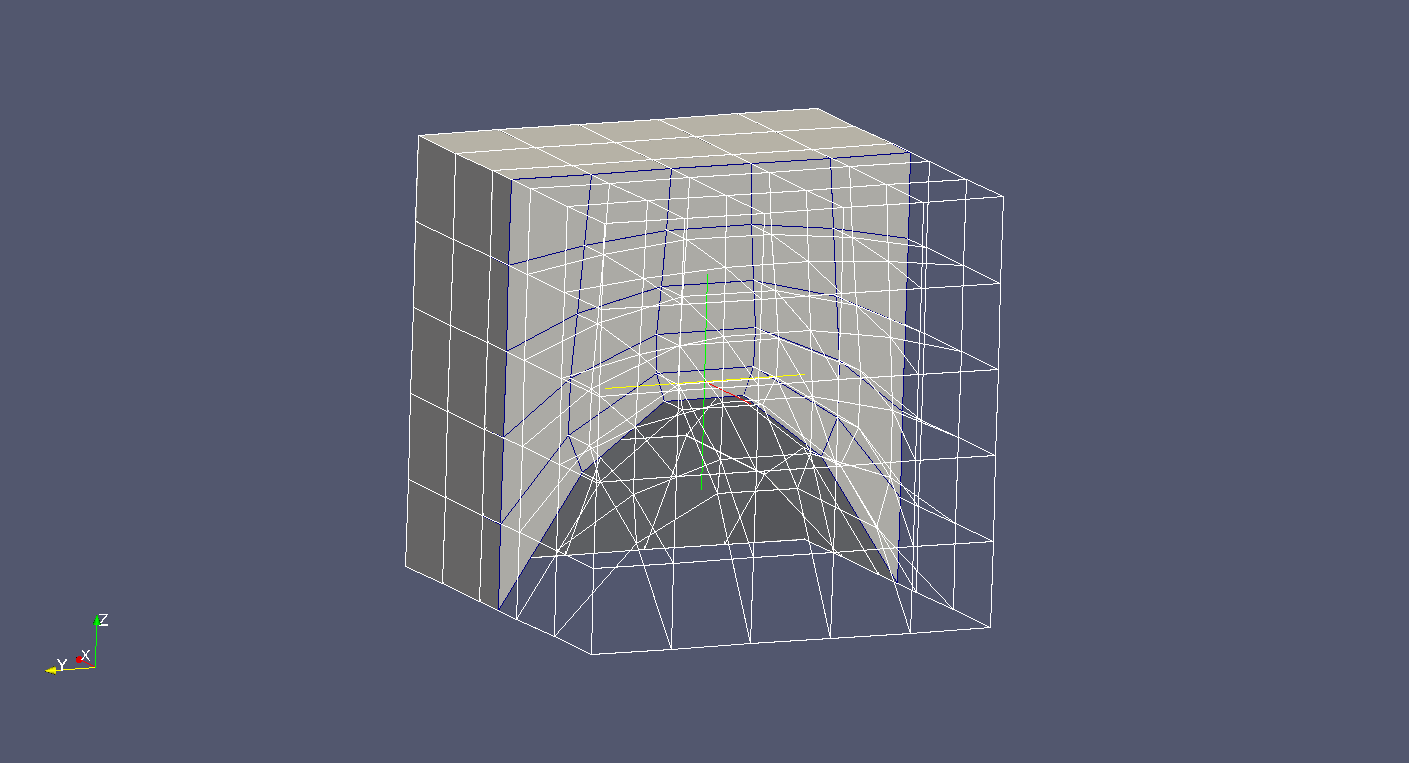
\includegraphics[width=4in]{par-hex-smoothed.eps}
\caption{Untangled and smoothed hexahedral mesh.}
\label{fig:par_hex_smoothed}
\end{center}
\end{figure*}

\subsection{Example: Using \texttt{Mesquite::Mesquite::MsqIMeshP}}

Similar to the example in Section \ref{sec:parallel-example-1}, this example uses the \texttt{LaplaceWrapper} wrapper in parallel to improve element shape.  However, this example assumes that either the iMeshP implementation is partitioning or that it is reading some pre-defined partitioned mesh and it relies on the iMeshP implementation to create ghost elements, assign global vertex IDs, etc.  

An implementation of the iMesh and iMeshP APIs must be provided for this example to work.  Mesquite can use these APIs, but does not provide them.

\begin{verbatim}
/* Mesquite includes */
#include <Mesquite.hpp>
#include <MsqIMeshP.hpp>
#include <ParallelMeshImpl.hpp>
#include <ParallelHelper.hpp>
#include <MsqError.hpp>
#include <LaplaceWrapper.hpp>

/* other includes */
#include <mpi.h>
#include <iostream>
using namespace std;
  
int main( int argc, char* argv[] )
{
  const char input_file[] = "testmesh";
  const char output_file[] = "smoothmesh";

  /* init MPI */
  int rank, nprocs;
  if (MPI_SUCCESS != MPI_Init(&argc, &argv)) {
    cerr << "MPI_Init failed." << endl;
    return 2;
  }
  MPI_Comm_rank(MPI_COMM_WORLD, &rank);
  MPI_Comm_size(MPI_COMM_WORLD, &nprocs);

  /* create a new instance of the iMesh database */
  int ierr;
  iMesh_Instance mesh;
  iMesh_newMesh(NULL, &mesh, &ierr, 0); 
  if (iBase_SUCCESS != ierr) return ierr;
  iBase_EntitySetHandle root_set;
  iMesh_getRootSet(mesh, &root_set, &ierr);
  if (iBase_SUCCESS != ierr) return ierr;

  /* create a partition instance in which to read 
     the partitioned mesh */
  iMeshP_PartitionHandle partition;
  iMeshP_createPartitionAll(mesh, MPI_COMM_WORLD, 
                            &partition, &err);
  if (iBase_SUCCESS != ierr) return ierr;

  /* load mesh */
  iMeshP_loadAll(mesh, partition, root_set, input_file, 
                 NULL, &err, strlen(input_file), 0); 
  if (iBase_SUCCESS != ierr) return ierr;

  /* create 1 layer of ghost entities */
  iMeshP_createGhostEntsAll(mesh, partition, 3, 1, 1, 0, &err); 
  if (iBase_SUCCESS != ierr) return ierr;

  /* create MsqIMeshP instance */
  Mesquite::MsqError err;
  Mesquite::MsqIMeshP parallel_mesh(mesh, partition, root_set, 
                                    iBase_REGION, err);
  if (err) {cerr << err << endl; return 1; }

  /* do Laplacian smooth */
  LaplaceWrapper optimizer;
  optimizer.run_instructions(&parallel_mesh, err);
  if (err) {cerr << err << endl; return 1; }

  /* write mesh */
  iMeshP_saveAll(mesh, partition, root_set, output_file, 
                 NULL, &ierr, strlen(output_file), 0);  
  if (iBase_SUCCESS != ierr) return ierr;
  
  /* cleanup */
  iMeshP_destroyPartitionAll(mesh, partition, &ierr); 
  if (iBase_SUCCESS != ierr) return ierr;
  iMesh_dtor(mesh, &ierr); 
  if (iBase_SUCCESS != ierr) return ierr;
  MPI_Finalize();
  return 0;
}
\end{verbatim}


%%
% This section describes in high level terms how an application uses Zoltan
% 
\chapter{Using the Zoltan library}
\label{cha:using}


\section{Overview}

The Zoltan library is a C library that you can link with your C,
C++ or Fortran application.  Details of the C++ and Fortran bindings
are provided in the User's Guide 
(\url{http://www.cs.sandia.gov/Zoltan/ug_html/ug.html}).
Because Zoltan uses MPI for communication, you must link your application
with the Zoltan library and with MPI.

The following points summarize the interface between your
application and the Zoltan library:

\begin{itemize}
\item Your parallel application must have a global set of IDs that uniquely identify each object that will be included in the partitioning.  Zoltan is flexible about the data type or size of your IDs.
\item You make a call to the Zoltan library to create a load balancing instance or handle.  All subsequent interactions with Zoltan related to this partitioning problem are done through this handle.  
\item You set parameters that state which partitioning method you wish Zoltan to use, how you want the method to behave, and what type of data you will be providing.
\item You create functions that Zoltan can call during partitioning to obtain your data.  You provide the names of these functions to Zoltan.
\item When you want to partition or repartition your data, all processes in your parallel application must call Zoltan.  When Zoltan returns, each process will have lists of the 
IDs of the data it must move to another process and of the data it will receive from 
other processes.  You must free these lists when you are done with them.
\item The Zoltan functions that you call will return success or failure information.
\end{itemize}

Most Zoltan users will only use the partitioning functions of Zoltan.  But Zoltan provides
some other useful capabilities as well, such as functions to aid with data migration, and
global data dictionaries to locate the partition holding a data object.  
After discussing the partitioning interface, we will briefly introduce those capabilities.

\section{Initializing and releasing Zoltan}

Every process in your parallel application must initialize Zoltan once
with a call to \textbf{Zoltan\_Initialize}.  Every
partitioning instance that is created with \textbf{Zoltan\_Create} must be freed at
the end with \textbf{Zoltan\_Destroy}.  And all lists returned by
Zoltan must be freed with \textbf{Zoltan\_LB\_Free\_Part}.  These functions
are defined in the User's Guide at
\url{http://www.cs.sandia.gov/Zoltan/ug\_html/ug\_interface\_init.html}
and they are are illustrated in each of the examples in chapter ~\ref{cha:ex}.

\section{Application defined query functions}

To make Zoltan easy to use, we do not impose any particular data structure 
on an application, nor do we require an application to build a particular 
data structure for Zoltan. Instead, Zoltan uses a callback function interface, 
in which Zoltan queries the application for needed data. The application must 
provide simple functions that answer these queries.

To keep the application interface simple, we use a small set of callback functions 
and make them easy to write by requesting only information that is easily accessible 
to applications. For example, the most basic partitioning algorithms require only 
four callback functions. These functions return the number of objects owned by a 
processor, a list of weights and IDs for owned objects, the problem's dimensionality, 
and a given object's coordinates. More sophisticated graph-based partitioning 
algorithms require only two additional callback functions, which return the number 
of edges per object and edge lists for objects.

The User's Guide 
(\url{http://www.cs.sandia.gov/Zoltan/ug\_html/ug\_query.html})
provides detailed prototypes for application defined query functions.
Several working examples of query functions can be found in this document,
for example in the Recursive Coordinate Bisection section (\ref{sec:rcb});

\section{Using parameters to configure Zoltan}

The behavior of Zoltan is controlled by several parameters and debugging-output 
levels. 
For example, you will set the parameter \textbf{NUM\_GID\_ENTRIES} to the
size of your application's global IDs, and you will set \textbf{DEBUG\_LEVEL}
to indicate how verbose you want Zoltan to be.
These parameters can be set by calls to \textbf{Zoltan\_Set\_Param}. Reasonable 
default values for all parameters are specified by Zoltan. Many of the parameters 
are specific to individual algorithms, and are listed in the descriptions of those 
algorithms in the User's Guide 
(\url{http://www.cs.sandia.gov/Zoltan/ug\_html/ug\_param.html}).

Each example in the next chapter (\ref{cha:ex}) includes code that sets 
general parameters and parameters for specific algorithms.

\section{Errors returned by Zoltan}

All interface functions, with the exception of \textbf{Zoltan\_Create}, return an 
error code to the application. The possible return codes are defined in 
\textbf{include/zoltan\_types.h} and Fortran module \textbf{zoltan}.

They are:

\begin{description}
\item [ZOLTAN\_OK] Function returned without warnings or errors.
\item [ZOLTAN\_WARN] Function returned with warnings. The application will probably be able to continue to run.
\item [ZOLTAN\_FATAL] A fatal error occured within the Zoltan library.
\item [ZOLTAN\_MEMERR] An error occurred while allocating memory. When this error occurs, the library frees any allocated memory and returns control to the application. If the application then wants to try to use another, less memory-intensive algorithm, it can do so.
\end{description}

\section{Additional functionality provided by Zoltan}

The Zoltan library includes many functions, in addition to its
partitioning codes, which are designed to aid parallel
large-data message passing applications.

While the focus of this tutorial is partitioning, we list these additional
capabilities here.  Most are described more fully in the User's Guide.
Where examples of use exist in the source code, we will point that out.

\begin{description}
\item [Data migration]
Existing applications that are being ported to Zoltan may already contain code to 
redistribute data across a parallel application.  However new codes may wish to
use Zoltan's data migration capabilities.  The application must supply functions
to pack and unpack the data.  Zoltan can either do the data migration automatically
after computing the new partitioning, or the application can explicitly call
\textbf{Zoltan\_Migrate} to perform the migration.  
Details and examples can be
found in the User's Guide
(\url{http://www.cs.sandia.gov/Zoltan/ug\_html/ug\_interface\_mig.html}).


\item [Distributed directory utility]
The owner (i.e. the processor number) of any computational object is subject to 
change during load balancing. An application may use this directory utility to 
manage its objects' locations. A distributed directory balances the load (in terms 
of memory and processing time) and avoids the bottle neck of a centralized directory design.
This distributed directory module may be used alone or in conjunction with Zoltan's 
load balancing capability and memory and communication services.
Details of this feature can be found in the User's Guide
(\url{http://www.cs.sandia.gov/Zoltan/ug\_html/ug\_util\_dd.html}).

\item [Timers]
\textbf{Zoltan\_Timer\_Create} is a useful function 
that creates a platform independent
timer that can be used by a parallel application.  The application can
specify, for each timer, whether timing checks should involve a
global barrier or not.  The Zoltan timer is not documented in the User's
Guide, but the example \textbf{examples/C/zoltanExample1.c} uses it.

\item [Unstructured communication]
The unstructured communication package provides a simple interface for 
doing complicated patterns of point-to-point communication, such as those 
associated with data remapping. This package consists of a few simple functions 
which create or modify communication plans, perform communication, and destroy 
communication plans upon completion. The package has proved useful in a 
variety of different applications. For this reason, it is maintained as a separate 
library and can be used independently from Zoltan.
Details of this feature can be found in the User's Guide
(\url{http://www.cs.sandia.gov/Zoltan/ug\_html/ug\_util\_comm.html}).

\item [Memory allocation wrappers]
This package consists of wrappers around the standard C memory allocation and 
deallocation routines which add error-checking and debugging capabilities. These 
routines are packaged separately from Zoltan to allow their independent use in other 
applications. 
They are described more fully in the User's Guide
(\url{http://www.cs.sandia.gov/Zoltan/ug\_html/ug\_util\_mem.html}).

\item [Parallel ordering]
With the \textbf{Zoltan\_Order} function,
Zoltan provides limited capability for ordering a set of objects, typically 
given as a graph.
This feature is described more fully in the User's Guide
(\url{http://www.cs.sandia.gov/Zoltan/ug\_html/ug\_interface\_order.html}).

\item [Parallel coloring]
Zoltan provides limited capability for coloring a set of objects, typically given 
as a graph. In graph coloring, each vertex is assigned an integer label such 
that no two adjacent vertices have the same label. 
This feature is described more fully in the User's Guide
(\url{http://www.cs.sandia.gov/Zoltan/ug\_html/ug\_interface\_color.html}).
\end{description}


%\chapter{Extending Mesquite}  \label{sec:extensions}

% \section{Mesquite Programming Framework}
% 
% \subsection{Mesquite Repository} 
% 
% The CVS repository is currently located on the unix NFS at mcs.anl.gov, for example log on to
% 'shakey.mcs.anl.gov' and go to the directory '/home/mesquite/cvs'; the name of the CVS module is
% 'mesquite'.
% 
% Access to the mesquite repository requires an Argonne MCS account, which can be granted through Todd
% Munson, among others: tmunson@mcs.anl.gov .
% One way to use the cvs directory at argonne is through the ssh protocol, i.e. define the environment
% variable 'CVS\_RSH' to be 'ssh' and for example, checking out a working copy would require the
% following command, where :ext: will require CVS to consult the 'CVS\_RSH' variable: 
% \begin{verbatim}
% cvs -d :ext:username@shakey.mcs.anl.gov:/home/mesquite/cvs co mesquite
% \end{verbatim}
% 
% \subsection{Mesquite Makefile} 
% 
% The mesquite makefile is \emph{not} a recursive makefile, i.e. a makefile that tells sub-directories
% to execute their own makefile. Instead, it includes all variables from sub-directories into one main
% makefile located in the main mesquite/ directory and called GNUmakefile.
% 
% Here we describe simple procedures needed for code development.
% 
% \subsubsection{Adding a header file within an existing directory}
% 
% Since adding a header file (.hpp) does not require to compile an extra objet file, no action is
% needed in order for the makefile to use the header file. Just run 'gmake clean; gmake' in order for
% the makefile to rerun its symbolinc links section or altenatively, create a symbolic link manually from
% 'mesquite/includeLinks' to the new header file.
% 
% \subsubsection{Adding a file within an existing directory}
% 
% When adding a '.cpp' file to an existing directory,  one needs to notify the makefile that a new
% object file (.o) needs to be compiled. This is not done automatically in order to provide some
% versatility.
% 
% Simply edit the 'MakefileVariables.inc' file within the directory where your new .cpp file has been added. The first
% variable defines the current directory, let's call it CURRENTDIR. The second variable describes the
% sources in the present directory (let's call it CONTROLSRC): that's the variable you need to add
% your new file name to. For example, the MakefileVariables.inc file used to start with: 
% \begin{verbatim}
% CURRENTDIR = $(srcdir)/dir1
% 
% CURRENTSRC = $(CURRENTDIR)/file1.cpp \
%             $(CURRENTDIR)/file2.cpp
% \end{verbatim}
% and it now starts with:
% \begin{verbatim}
% CURRENTDIR = $(srcdir)/dir1
% 
% CURRENTSRC = $(CURRENTDIR)/file1.cpp \
%             $(CURRENTDIR)/file2.cpp \
%             $(CURRENTDIR)/file3.cpp
% \end{verbatim}
% That's it, you can now run gmake from the 'mesquite'directory 
% and it will pick up all dependencies and include your new file in
% the mesquite library.
% 
% \subsubsection{Adding a directory within the source tree}
% 
% To add a new directory to the source tree, you need two files 
% in the new directory: the 'MakefileVariables.inc' file and
%  the 'MakefileTargets.inc' file. For example, copy those files from 
%  the mesquite/src/Control directory and replace the string 'CONTROL' in 
% those two files by a string unique to your new directory (for example 
% 'CONTROLSRC' becomes 'NEWDIRSRC'). Make sure not to miss any querry/replace.
% 
% You can now define the new directory location and the new source files 
% names in the 'MakefileVariables.inc' file, as explained in the 
% previous section.
% 
% Finally, you need to add the new directory to the MODULENAMES variable in the main makefile
% mesquite/GNUmakefile, and you can run gmake. 
% 
% \subsubsection{Adding a new driver code}
% 
% To add a new driver code (e.g. mesquite/testSuite/test\_1/main.cpp), 
% copy to a new directory under 'mesquite/testSuite/' the
% 'mesquite/testSuite/test\_1/Makefile.inc' file and change 
% within that file the string TEST1 to a new unique string. 
% Now, add the new directory to the TESTNAMES variable within 
% 'mesquite/GNUmakefile'. 
% 
% To compile the new driver, go to the main 'mesquite/' directory and type:
% \begin{verbatim}
% gmake mesquite/yournewdir/main
% \end{verbatim}
% where main will be the executable name (note that this name can be 
% changed in the third variable in Makefile.inc).
% 
% 
% \subsection{Unit Test Suite Makefile}
% 
% The unit test suite, located in 'mesquite/testSuite/unit/' has its 
% own makefile. It is not as robust as the main mesquite makefile and can 
% be improved (it does not pick up all dependencies properly).
% 
% To compile the unit test suite, go into 'mesquite/testSuite/unit/' 
% and type 'gmake'. 
% 
% As you modify the test suite and mesquite in parallel, you might 
% need to use 'gmake clean; gmake' to pick up some dependencies ... 
% or you could improve the makefile. 
% 
% 
% \subsection{Directory Structure}
% 
% The base directory of the Mesquite project contains several
% sub-directories which are intended to help keep the project's
% files organized.  Some of the sub-directories themselves are
% also sub-divided.  Below are descriptions of the first level
% of sub-directories ({\it i.e.,} the directories contained in the
% base directory).
% \begin{enumerate}
% \item doc:  Contains a version of this document and a version of
% the developer's documentation generated with doxygen (TODO: acknowledge
% doxygen).
% \item include:  Contains the Mesquite header file, ``Mesquite.hpp.''
% \item includeLinks:  Contains soft links to the other header files
% used within Mesquite.  
% \item lib:  The location where the Mesquite library, ``libmesquite.a,'' is
% stored.
% \item meshFiles:  Contains example meshes that are used in some of
% the test cases.
% \item mswindow:  Contains the project file for compiling with Visual C++
% (TODO: VC++ trademark statement???).
% \item obj:  The directory where the object files are placed.
% \item src:  Contains the Mesquite source code and header files (except for
% Mesquite.hpp).
% \item testSuite:  Contains example driver codes which use Mesquite.  These
% test cases can only be ran when linked with the correct libraries (generally,
% AOMD or MDB).
% \end{enumerate}
% 
% \subsection{Code Testing Framework}
% 
% Another integral part of the Mesquite framework is the code testing
% infrastructure.  Several testing methodologies have been included
% within Mesquite. Unit testing is extensively used to facilitate
% development and ensure low-level robustness. Functional testing is
% used to ensure that user case scenarios run smoothly.
% 
% We use a broad definition for unit tests in Mesquite. Any test
% performed on a class without need for the entire Mesquite framework is
% considered a unit test. This encompasses simple assertions like
% checking the result of the multiplication of a matrix $A \in
% \Bbb{R}^{3 \times 3}$ by a vector $v \in \Bbb{R}^{3}$ to more complex
% assertions such as checking that a concrete \texttt{QualityImprover}
% correctly repositions a free vertex in a simple patch for a given
% objective function and quality metric.
% 
% Mesquite uses a readily available testing framework called CppUnit
% \cite{cppunit} --- essentially the well known jUnit testing framework
% ported to C++.  Using the unit testing methodology allows the
% developers to write far more robust code.
% 
% Applications using Mesquite may also find the testing framework useful
% when verifying their additions to the code. In particular,
% applications that prefer to implement Mesquite's mesh interface
% instead of using the TSTT mesh interface will want to
% check their implementation with the corresponding unit test collection
% available in Mesquite. In addition, analytic gradient and Hessian
% implementations can be checked against the numerical version provided
% by the {\tt QualityMetric} base class using readily available unit
% tests.
% 
% In addition to unit tests, the Mesquite test suite also includes
% a range of functional tests.  While these tests also use the
% CppUnit framework, they differ from unit tests in that 
% functional tests require the entire Mesquite framework.
% The functional tests are complete and often complex mesh
% optimization problems.  These tests are intended to ensure that
% the individual units of the Mesquite code work together correctly.
% Performing these tests not only helps
% validate the code but also allows developers to evaluate the
% effects of code modifications in terms of Mesquite's accuracy
% and efficiency on `real world' problems.

\section{Defining New Concrete Classes}

% \begin{verbatim}
% Explain that we only mention the truly polymorphic extensions. 
% Extensions that require not only an additional class, 
% but also other changes in the code (switches) are 
% not discussed int he user manual for now. This is a 
% reference manual issue. Give explicit examples of difficult things. 
% \end{verbatim}

The Mesquite architecture uses as much dynamic polymorphism in the
form of inheritance and virtual functions as is possible without
degrading performance.  This allows developers to add new
functionality to Mesquite by inheriting from the appropriate abstract
class and implementing its interface (i.e. its abstract virtual
functions).  We note that the mesh entities, defined by class {\tt
MsqMeshEntity}, are the only exception in our architecture.  Mesh
entities, i.e. triangles, tetrahedrons, quadrangles and hexahedrons,
are implemented in a single class, without the use of dynamic
polymorphism, to eliminate the performance impact of runtime
resolution.

\subsection{Adding a New Quality Metric} \label{sec:QualityMetricImpl}

The primary functionality associated with the {\tt QualityMetric}
class is the \texttt{evaluate\_element} or\texttt{evaluate\_vertex}  function which returns a single quality value
for a given mesh entity.

To implement a new quality metric, a user must inherit from the base
\texttt{QualityMetric} class and implement the `evaluate' function.
\texttt{ QualityMetric} provides a wide range of
functionality that allows the quality metrics to be defined in a
flexible way and therefore gives the user the ability to modify the
metric in a variety of ways.  For example, the condition number
quality metric for a quadrilateral or hexahedral element is computed
by evaluating the condition number at a number of sample points in the
element.  Mesquite allows the user to select which set of sample
points are used in this calculation ({\it e.g.}, the element's
vertices) and how these values are combined to form a single metric
value ({\it e.g.}, linear averaging).  Mesquite is currently being
extended to allow certain quality metrics to be referenced to a
non-isotropic element.

\subsection{Adding a New Objective Function}

\subsection{Adding a New Vertex Mover Algorithm}

A new vertex mover algorithm is defined by inheriting from the
\texttt{VertexMover} abstract class. The \texttt{VertexMover} class 
is an intermediate abstract classe, inheriting from the
\texttt{QualityImprover} class (see Figure \ref{fig:uml}),  which
essential functionality is to implement the \texttt{loop\_over\_mesh}
virtual function that shields the optimization algorithm developer
from the need to distinguish between local or global patches.  The
\texttt{VertexMover} base class also checks the outer termination
criterion to stop iterating over mesh subsets (see section
\ref{termination_section}) and updates the application mesh after
optimizing a patch.

The gathering of the mesh information from a \texttt{Mesh} into the patch is
carried out by the \texttt{PatchData} class, so that the
optimization algorithm receives the appropriate patch to improve
simply by inheriting from \texttt{QualityImprover}.  If needed, one can 
override the \texttt{set\_patch\_type} function to accept only specific
patch types.

% \subsection{Adding a New Topology Modifier Algorithm}





%\chapter{Troubleshooting}



%\chapter{Caveats, Limitations, and Disclaimers}

Input meshes may suffer quality dis-improvement in some cases due to
failures of the numerical algorithm. Users are advised to keep a copy
of their original mesh in case of such a failure.



\chapter{User Support}

\section{Mailing Lists}

An open mailing for discussion of Mesquite usage questions is available at
\href{mailto:mesquite@software.sandia.gov}{mesquite@software.sandia.gov}.  This list is open to all Mesquite users.  
Archived messages and subscription information are available on the list web 
page: \newline
\href{http://software.sandia.gov/mailman/listinfo/mesquite}{http://software.sandia.gov/mailman/listinfo/mesquite}.

%\section{Frequently Asked Questions}

\section{WWW Page}

The Mesquite WWW page is located at \newline
\url{http://www.cs.sandia.gov/optimization/knupp/Mesquite.html}.


\appendix

\chapter{The Mesquite Team}

The Mesquite team is composed of members from Sandia
National Laboratories (SNL), Lawrence Livermore National Laboratory (LLNL), 
and the University of Wisconsin--Madison (UW).\newline
 
\noindent The current Mesquite developement team includes: \newline

Lori Freitag-Diachin (Co-PI, LLNL), \newline

Patrick Knupp (Co-PI, SNL), and \newline

Jason Kraftcheck (UW).  \newline

\noindent Past developers and other significant contributors to
the development of Mesquite include:\newline

Michael Brewer (SNL), \newline

Ulrich Hetmaniuk (SNL), \newline

Thomas Leurent (ANL), \newline

Darryl Melander (SNL), and \newline

Todd Munson (ANL).  \newline

\noindent Current Mesquite developers can be contacted via e-mail at either 
the (private) developers' mailing list: 
\href{mailto:mesquite-developers@software.sandia.gov}
{Mesquite-Developers@software.sandia.gov},
or the (open) mailing list for all Mesquite users: 
\href{mailto:mesquite@software.sandia.gov}{Mesquite@software.sandia.gov}.


\chapter{Acknowledgments}

Mesquite is supported under the DOE SciDAC Interoperable Tools
and Petascale Simulation (ITAPS) project. 

%Terascale Simulation 
%Tools and Technology (TSTT) project \cite{tstt}.  

%{\it Funding sources (DOE SciDAC Program), Related activities
%(ITAPS, Cubit, Opt-MS), helpful folks (RPI for AOMD, ITAPS for MDB, LLNL
%for Overture tests, etc.}



\bibliographystyle{plain}
\bibliography{mesquite}


\end{document}


